% !TeX root = ../../Skript.tex
\cohead{\Large\textbf{Waagrechte Asymptoten}}
\fakesubsection{Waagrechte Asymptoten}
Jede Funktion vom Typ \(f(x)=a\cdot e^{kx}\) hat als Asymptote die x-Achse \(y=0\). Verschiebt man die Funktion nun um \(b\) in y-Richtung, so verschiebt sich die Asymptote ebenfalls um \(b\):
\begin{tcolorbox}\centering
	\textcolor{loestc}{\(f(x)=a\cdot e^{kx}+b\text{ hat die Asymptote }y=b\)}
\end{tcolorbox}
\begin{minipage}{\textwidth}
	\adjustbox{valign=t, padding =0ex 0ex 2ex 0ex}{\begin{minipage}{0.5\textwidth-2ex}
		\begin{minipage}{\textwidth}
			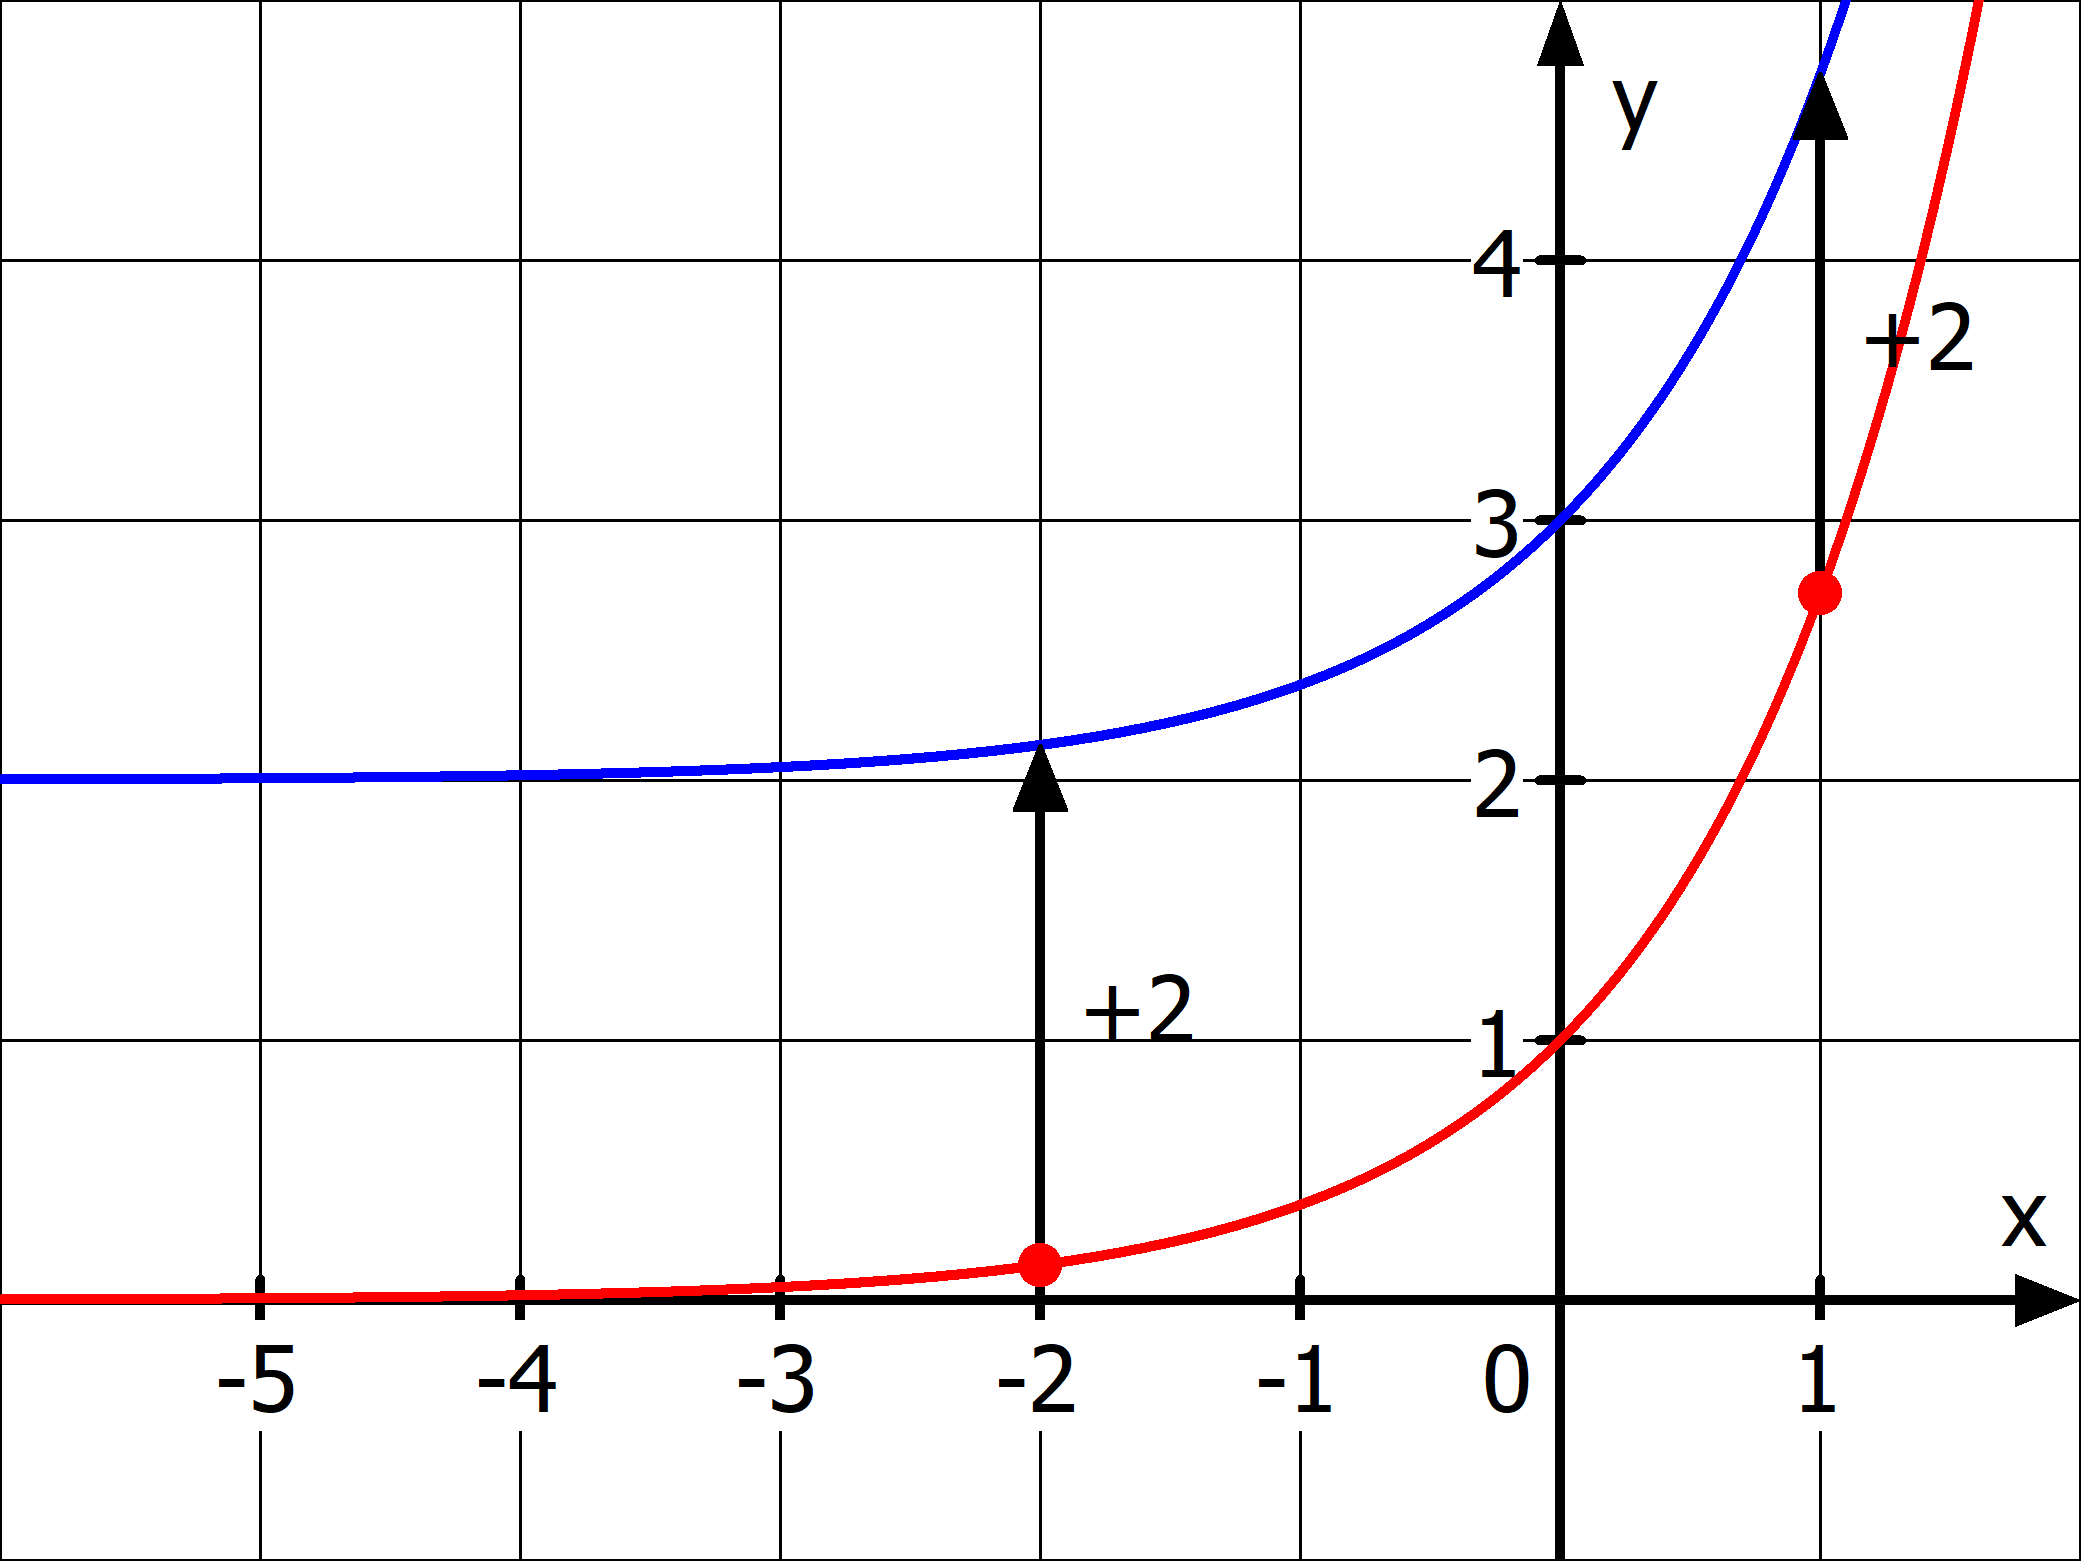
\includegraphics[width=\linewidth]{\eFkt/pics/versch1.png}
		\end{minipage}%

        \smallskip

		\textcolor{red}{\(f_1(x)=e^x\)} um \textcolor{blue}{2} nach oben verschoben:

		\textcolor{blue}{\(f_2(x)=e^x+2\)} mit Asymptote \textcolor{blue}{\(y=2\)}
	\end{minipage}}%
	\adjustbox{valign=t, padding =2ex 0ex 0ex 0ex}{\begin{minipage}{0.5\textwidth-2ex}
		\begin{minipage}{\linewidth}
            \iftoggle{qrcode}{%
                \settototalheight{\imgheight}{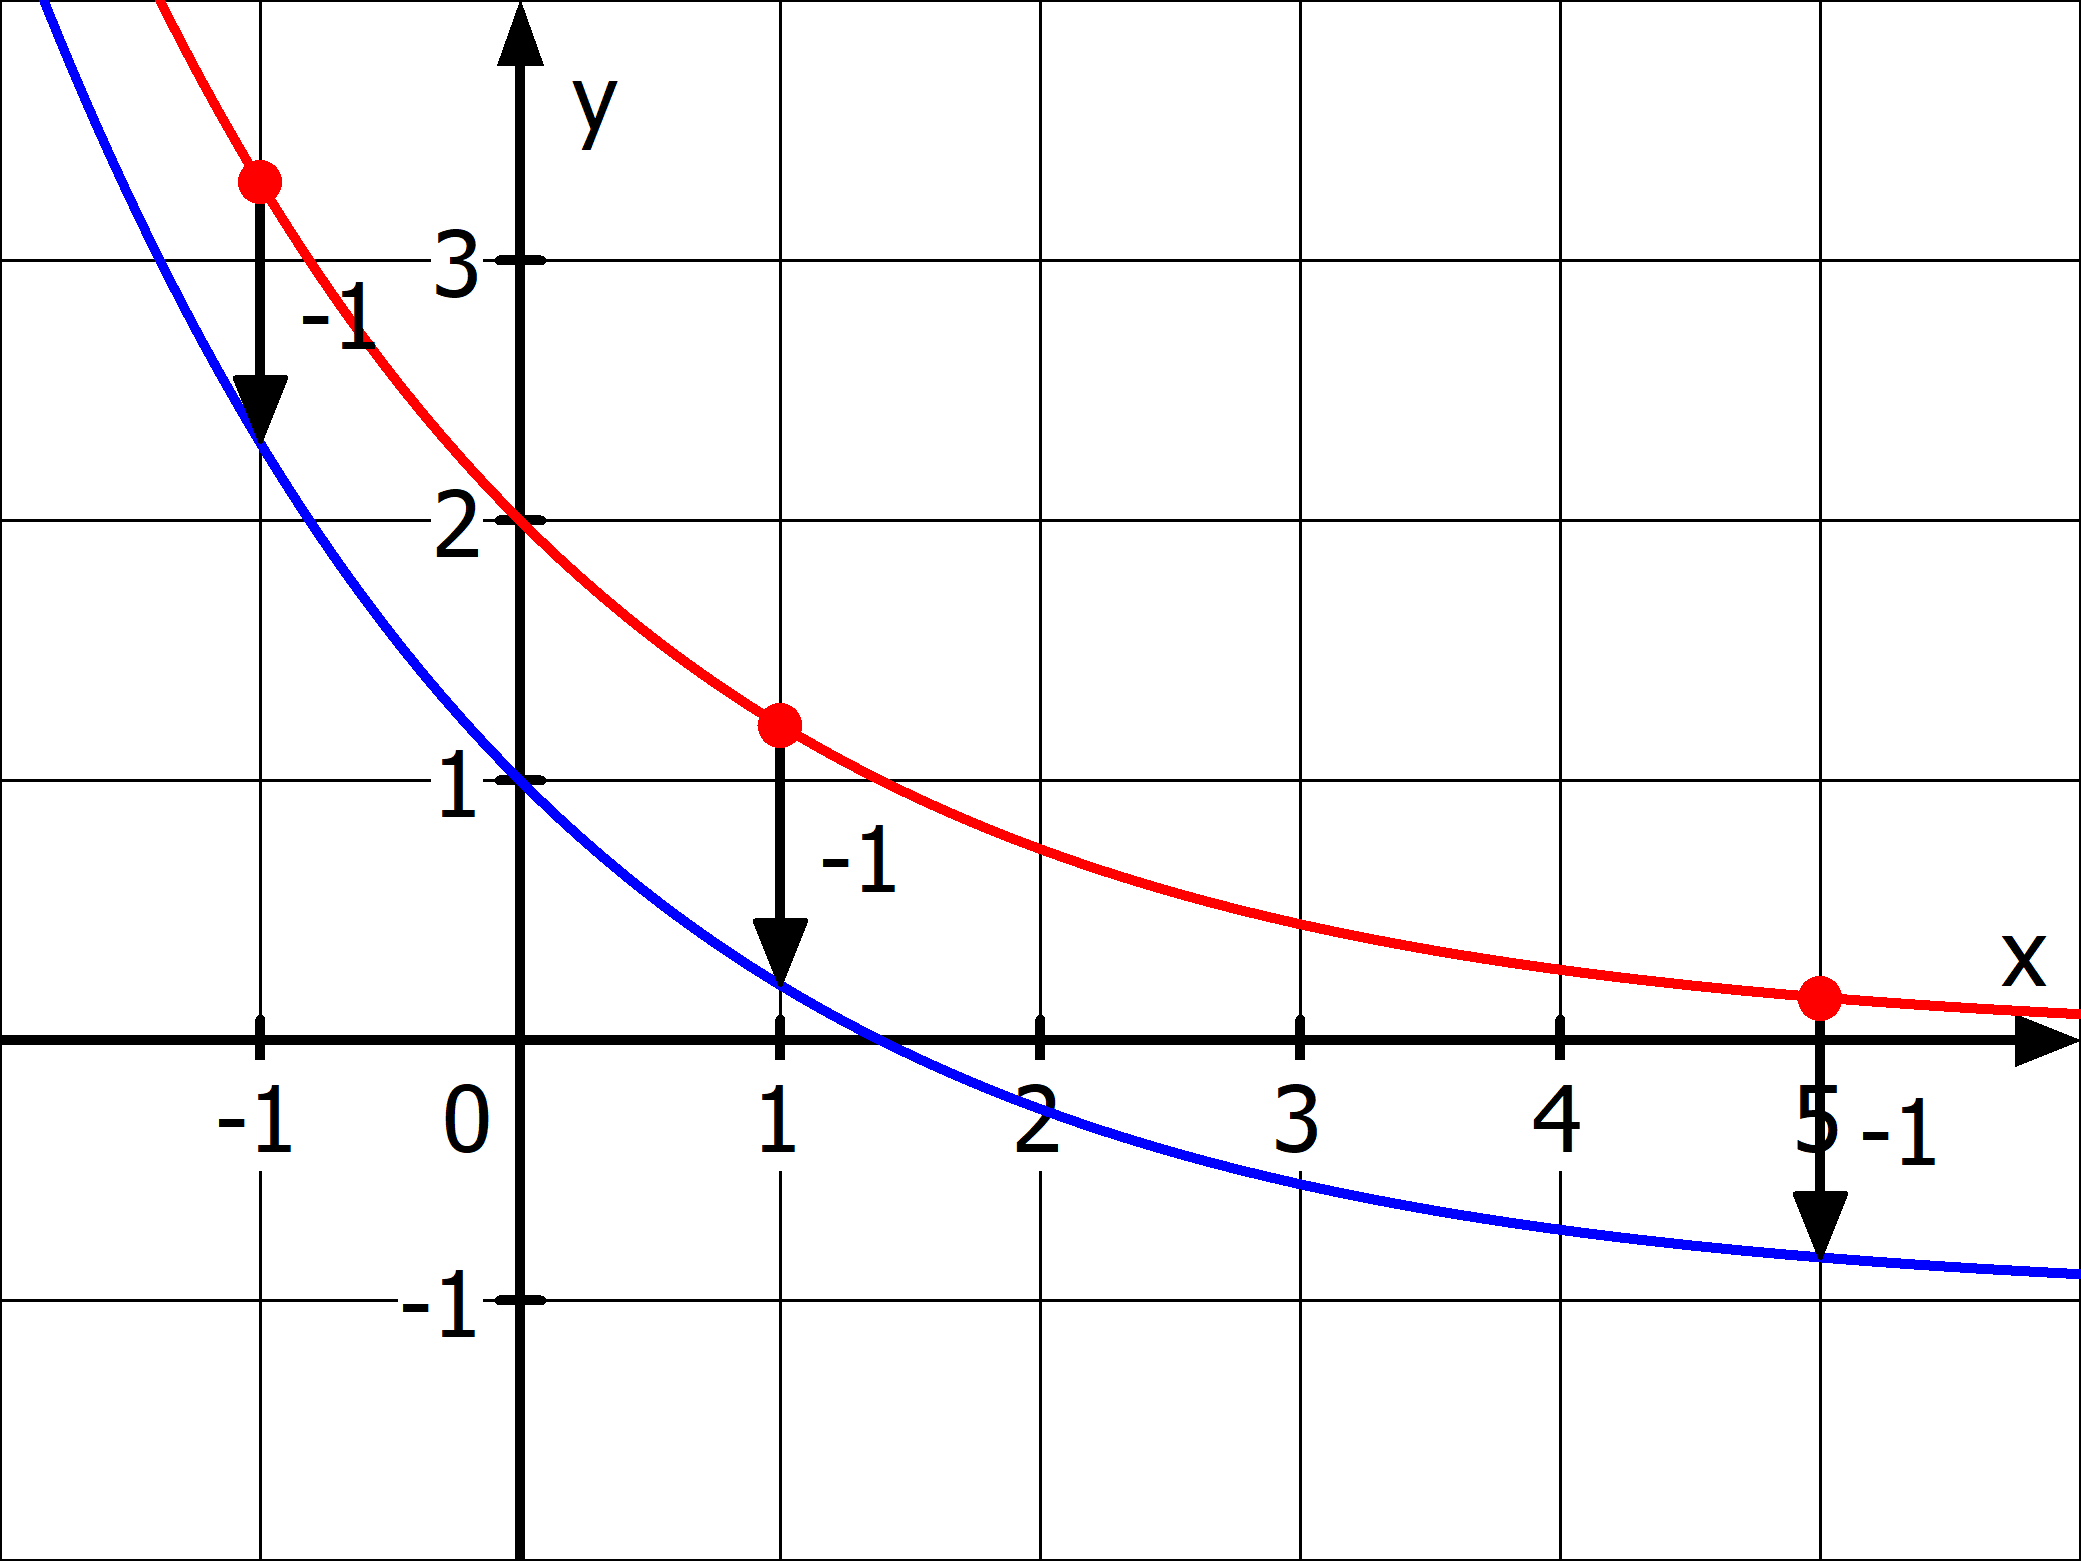
\includegraphics[width=\linewidth]{\eFkt/pics/versch2.png}}%
                \setlength{\qrheight}{2.5cm}%
                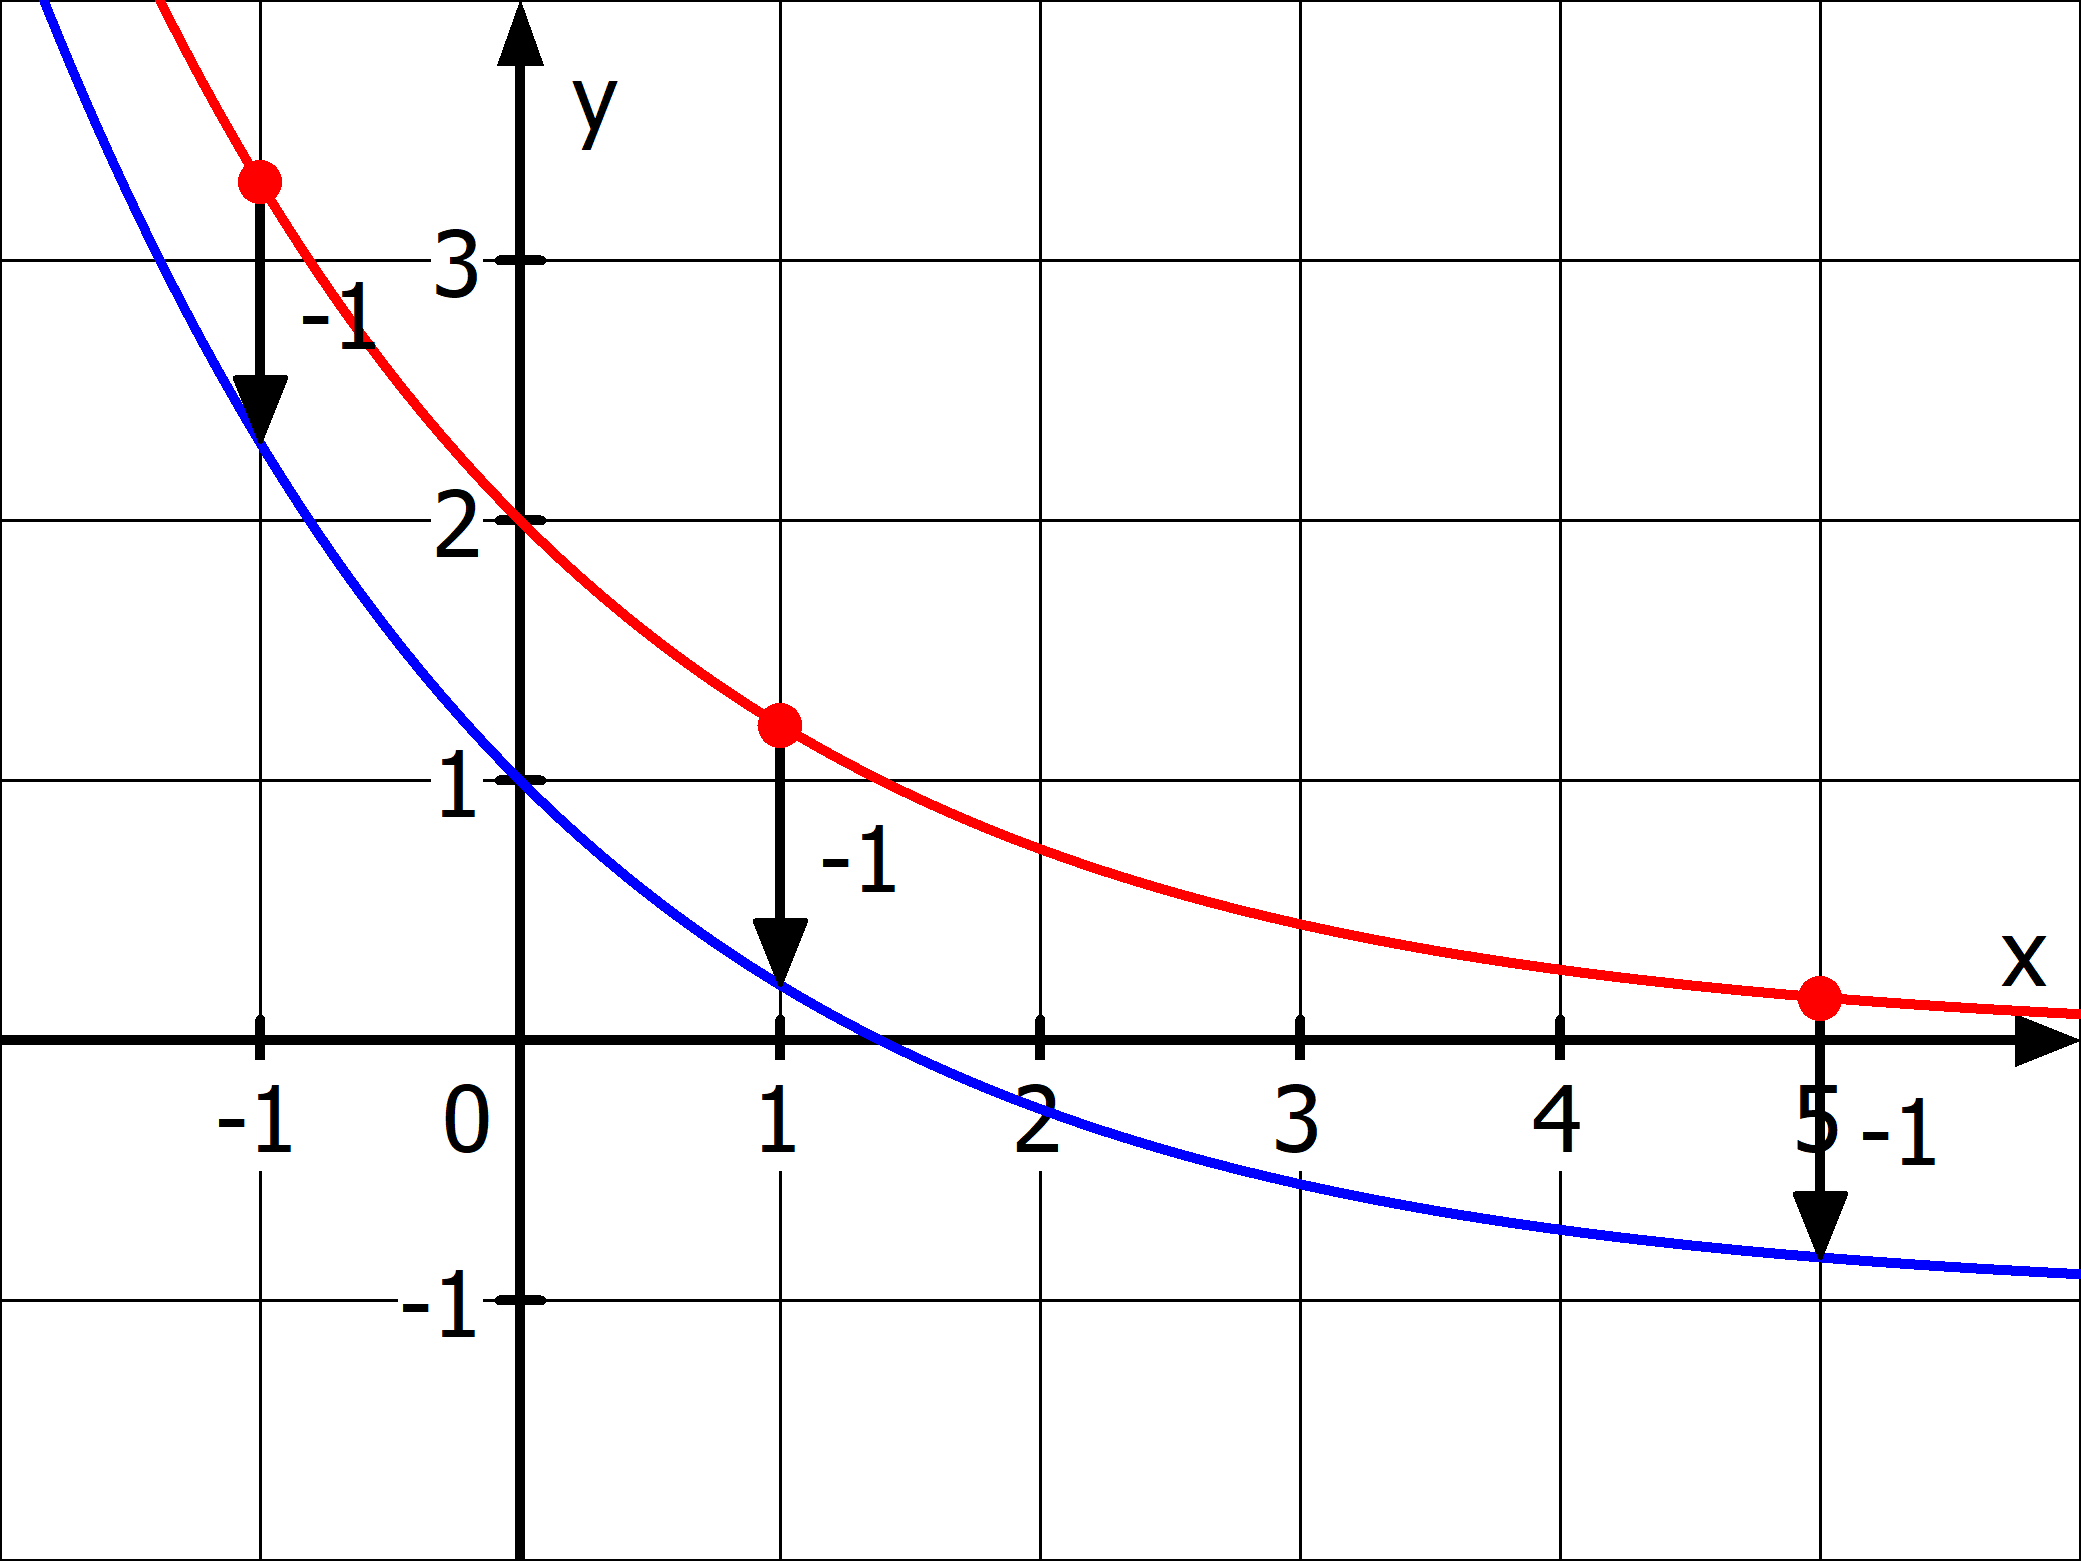
\includegraphics[width=\linewidth]{\eFkt/pics/versch2.png}%
                \raisebox{\imgheight-\qrheight}{\makebox[0pt][r]{\href{https://www.geogebra.org/m/xnzg5tn5}{
\includegraphics[height=\qrheight]{\eFkt/pics/waagrechteAsymptotenQR.png}}}}%
            }{%
                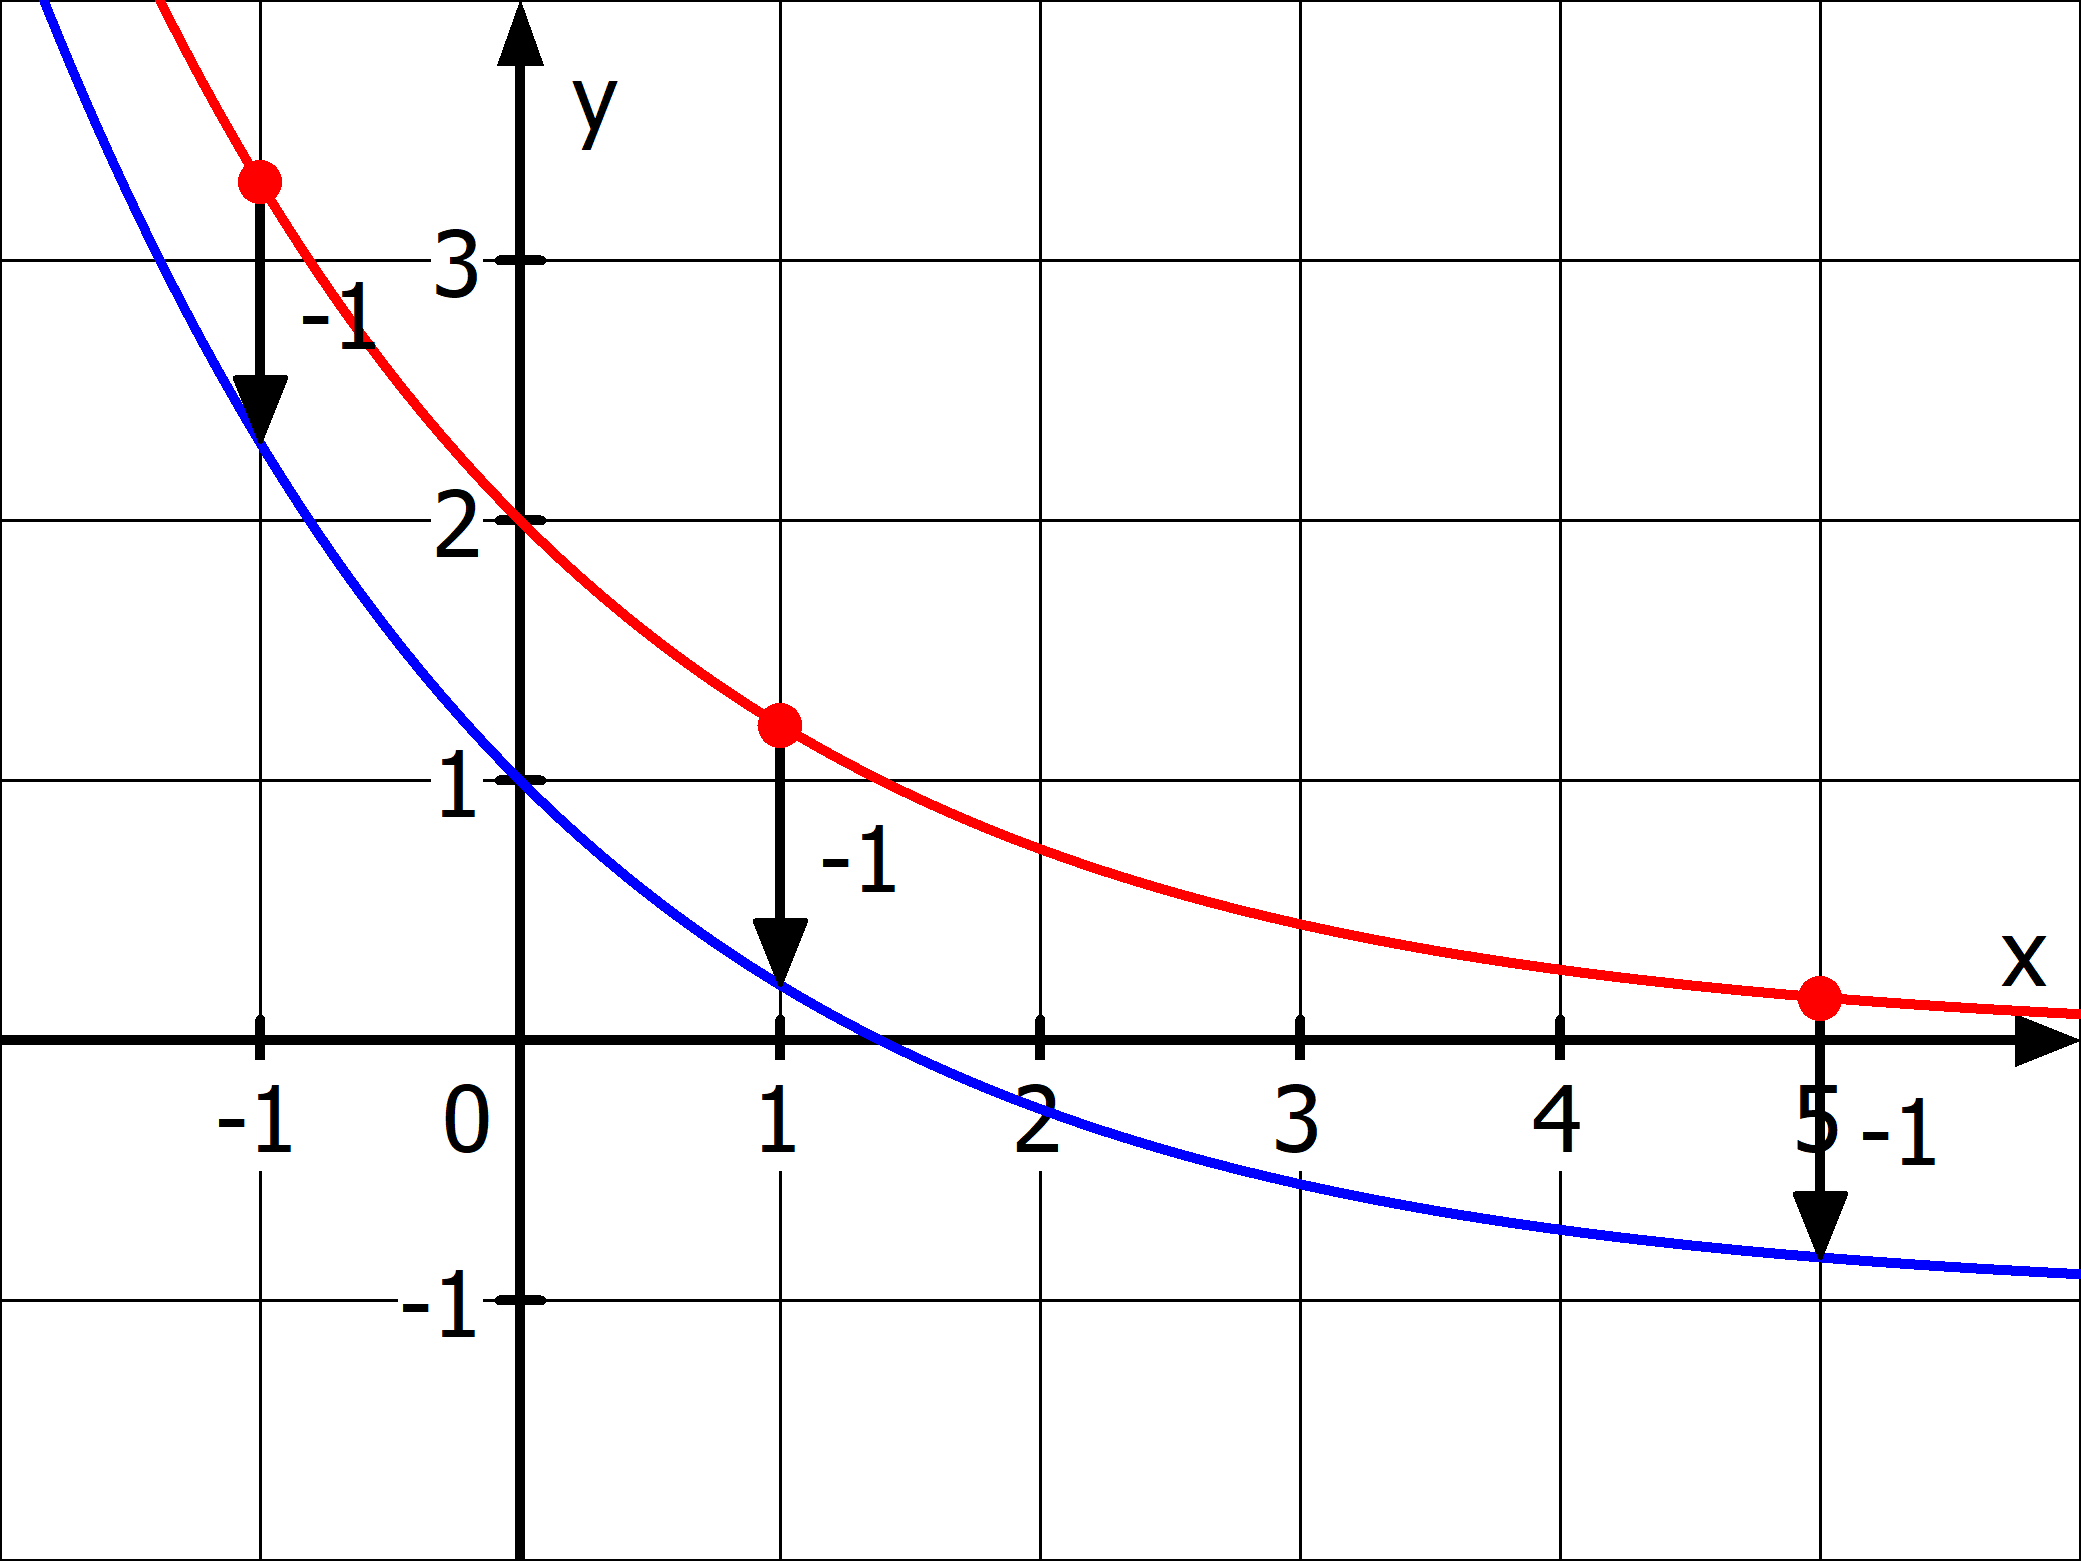
\includegraphics[width=\linewidth]{\eFkt/pics/versch2.png}
            }%
		\end{minipage}%

        \smallskip

		\textcolor{red}{\(f_3(x)=2e^{-0,5x}\)} um \textcolor{blue}{1} nach unten verschoben:

		\textcolor{blue}{\(f_4(x)=2e^{-0,5x}-1\)} mit Asymptote \textcolor{blue}{\(y=-1\)}
	\end{minipage}}%
\end{minipage}

\vspace{1cm}

%%%%%%%%%%%%%%%%%%%%%%%%%%%%%%%%%%
Für viele Aufgabenstellungen ist eine Skizze hilfreich, die sich wie folgt erstellen lässt. Als Beispiel verwenden wir \(f(x)=-2e^{\frac{1}{3}x}+3\):

\medskip

\begin{minipage}{\textwidth}
	\adjustbox{valign=t, padding =0ex 0ex 2ex 0ex}{\begin{minipage}{0.5\textwidth-2ex}
		\begin{enumerate}[label=\arabic*)]
			\setcounter{enumi}{0}
			\item Asymptote ablesen: \textcolor{blue}{\(y=b\)}
		\end{enumerate}%
	\end{minipage}}%
	\adjustbox{valign=t, padding =2ex 0ex 0ex 0ex}{\begin{minipage}{0.5\textwidth-2ex}
		\begin{enumerate}[label={}, leftmargin=*]
			\item Asymptote \textcolor{blue}{\(y=3\)}
		\end{enumerate}
	\end{minipage}}%
\end{minipage}\vspace{0.2cm}
%%%%%%%%%%%%%%%%%%%%%%%%%%%%%%%%%%%%%%%%%%%%%%%%%
\begin{minipage}{\textwidth}
	\adjustbox{valign=t, padding =0ex 0ex 2ex 0ex}{\begin{minipage}{0.5\textwidth-2ex}
		\begin{enumerate}[label=\arabic*)]
			\setcounter{enumi}{1}
			\item y-Achsenabschnitt berechnen:

			\textcolor{blue}{\(f(0)=a+b\)}
		\end{enumerate}
	\end{minipage}}%
	\adjustbox{valign=t, padding =2ex 0ex 0ex 0ex}{\begin{minipage}{0.5\textwidth-2ex}
		\begin{enumerate}[label={}, leftmargin=*]
			\item y-Achsenabschnitt:

			\textcolor{blue}{\(f(0)=-2e^{\frac{1}{3}\cdot 0}+3=-2+3=1\)}
		\end{enumerate}
	\end{minipage}}%
\end{minipage}\vspace{0.2cm}
%%%%%%%%%%%%%%%%%%%%%%%%%%%%%%%%%%%%%%%%%%%%%%%%%
\begin{minipage}{\textwidth}
	\adjustbox{valign=t, padding =0ex 0ex 2ex 0ex}{\begin{minipage}{0.5\textwidth-2ex}
		\begin{enumerate}[label=\arabic*)]\raggedright
			\setcounter{enumi}{2}
			\item Form an Hand der Vorzeichen von \(a\) und \(k\) bestimmen
		\end{enumerate}
	\end{minipage}}%
	\adjustbox{valign=t, padding =2ex 0ex 0ex 0ex}{\begin{minipage}{0.5\textwidth-2ex}
		\begin{enumerate}[label={}, leftmargin=*]
			\item Aus \(a=-2\) negativ und \(k=\frac{1}{3}\) positiv folgt, dass das Schaubild sich nach links von unten der Asymptote nähert und nach rechts gegen \(-\infty\) geht.
		\end{enumerate}
	\end{minipage}}%
\end{minipage}
%%%%%%%%%%%%%%%%%%%%%%%%%%%%%%%%%%%%%%%%%%%%%%%%%
\begin{minipage}{\textwidth}
	\adjustbox{valign=t, padding =0ex 0ex 2ex 0ex}{\begin{minipage}{0.5\textwidth-2ex}
		\begin{enumerate}[label=\arabic*)]\raggedright
			\setcounter{enumi}{3}
			\item Asymptote ins Koordinatensystem einzeichnen und y-Achsenabschnitt markieren
            \item Schaubild der Funktion skizzieren
		\end{enumerate}
	\end{minipage}}%
	\adjustbox{valign=t, padding =2ex 0ex 0ex 0ex}{\begin{minipage}{0.5\textwidth-2ex}
		\begin{minipage}[t]{\textwidth}
			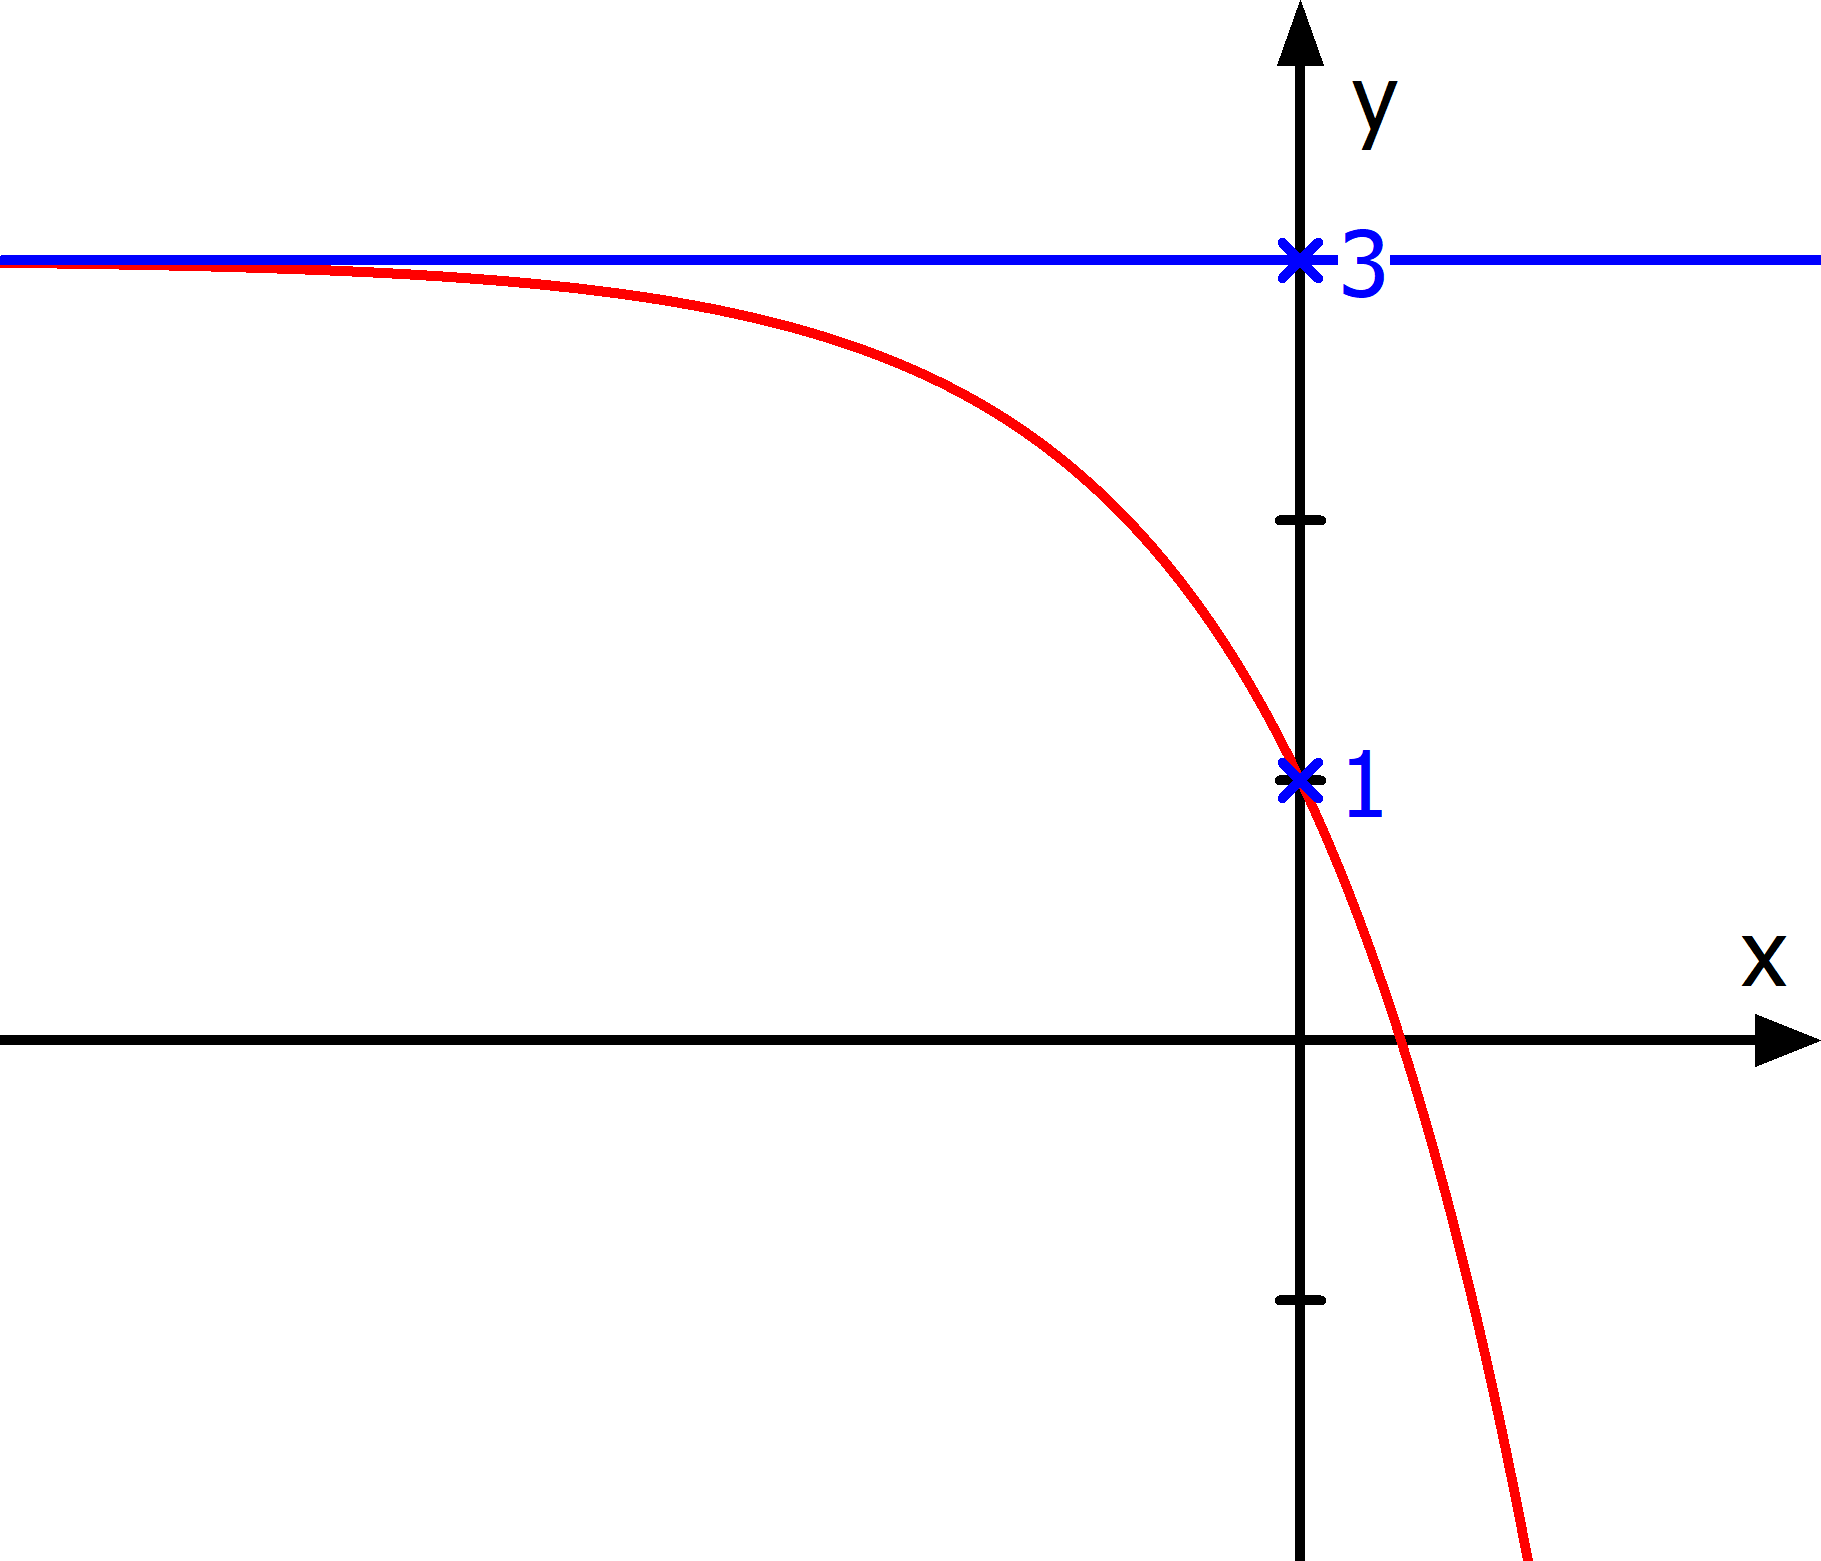
\includegraphics[width=\linewidth]{\eFkt/pics/verschBsp1.png}
		\end{minipage}
	\end{minipage}}%
\end{minipage}
%%%%%%%%%%%%%%%%%%%%%%%%%%%%%%%%%%%%%%%%%%%%%%%%%
%\begin{minipage}{\textwidth}
%	\adjustbox{valign=t, padding =0ex 0ex 2ex 0ex}{\begin{minipage}{0.5\textwidth-2ex}
%		\begin{enumerate}[label=\arabic*)]
%			\setcounter{enumi}{4}
%			\item Schaubild der Funktion skizzieren
%		\end{enumerate}
%	\end{minipage}}%
%	\adjustbox{valign=t, padding =2ex 0ex 0ex 0ex}{\begin{minipage}{0.5\textwidth-2ex}
%		\begin{minipage}[t]{0.95\textwidth}
%			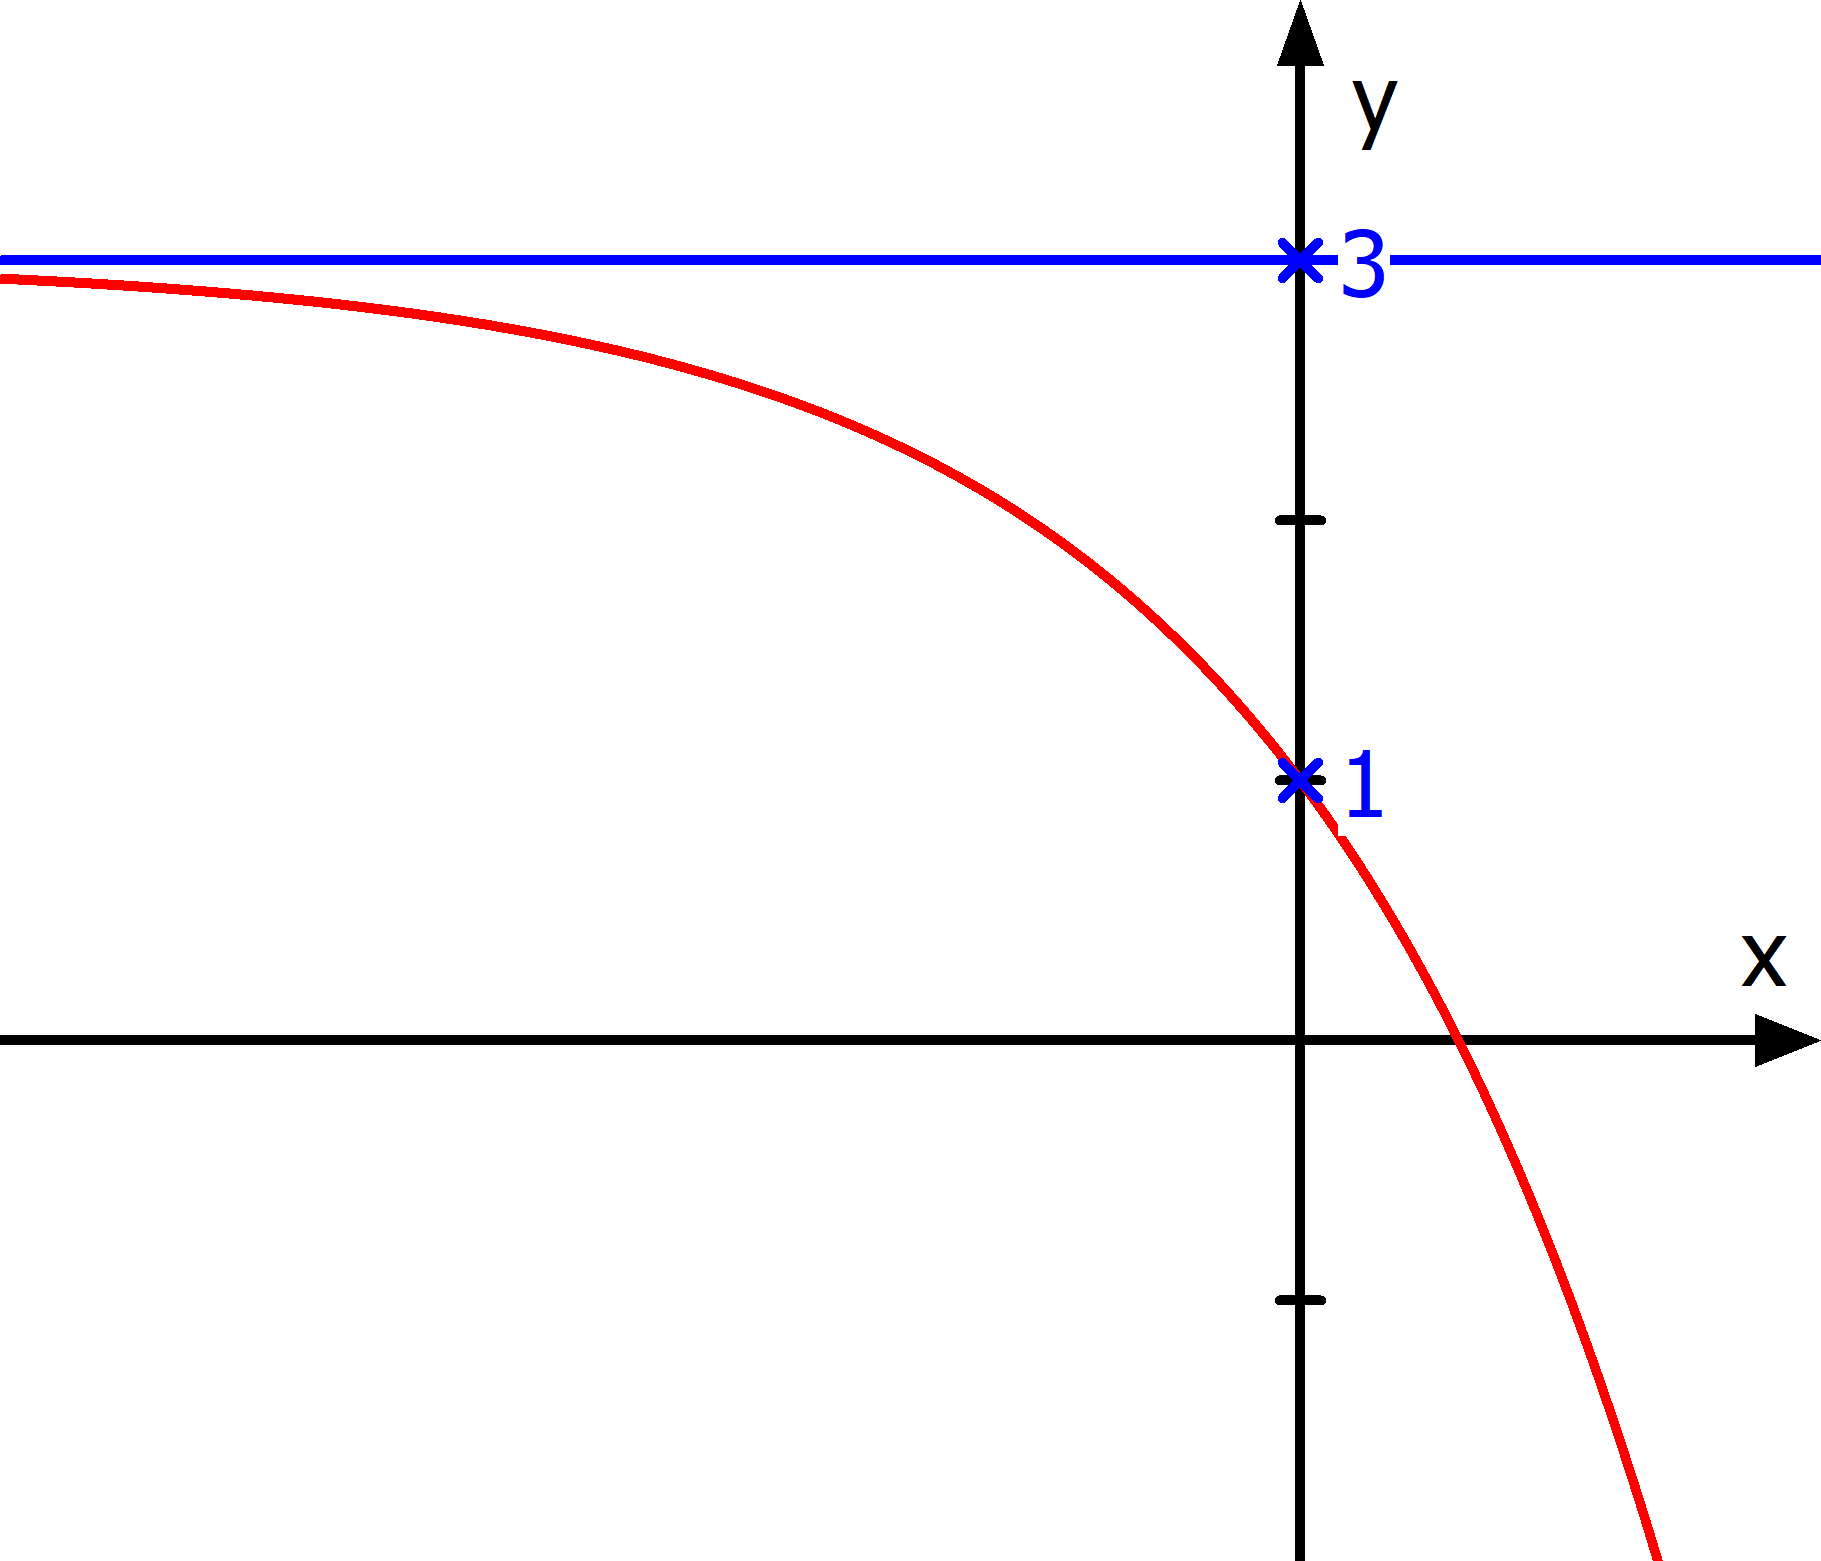
\includegraphics[width=.6\linewidth]{\eFkt/pics/verschBsp2.png}
%		\end{minipage}
%	\end{minipage}}%
%\end{minipage}
\newpage
%%%%%%%%%%%%%%%%%%%%%%%%%%%%%%%%%%%%%%%%%%%%%%%%%%%%%%%%%%%%%%%%%%%%%%%%%%%%%%%%%%%%%%%%%%%%%%%%%%%%%%
\begin{Exercise}[title={Bestimme den y-Achsenabschnitt, skizziere das Schaubild, gib die Asymptote, das Verhalten für \(x\rightarrow \pm\infty\) und die Monotonie an}, label=eFktA2]

	\begin{minipage}{\textwidth}
		\begin{minipage}{0.5\textwidth}
			\begin{enumerate}[label=\alph*)]
				\item \(f(x)=e^{-2x}-3\)
				\item \(f(x)=2e^{\frac{1}{2}x}+1\)
				\item \(f(x)=-3e^{2x}+6\)
				\item \(f(x)=-2e^{-7x}-1\)
				\item \(f(x)=\frac{5}{2}e^{2x}-2\)
				\item \(f(x)=-8e^{3x}+8\)
				\item \(f(x)=2e^{-\frac{3}{8}x}-5\)
				\item \(f(x)=-\frac{3}{2}e^{0,2x}+2\)
				\item \(f(x)=-5e^{-3,5x}+5\)
				\item \(f(x)=-8e^{0,3x}+6\)
				\item \(f(x)=2e^{-2x}+2\)
				\item \(f(x)=-6+4e^{-7x}\)
				\item \(f(x)=8-5e^{x}\)
			\end{enumerate}
		\end{minipage}%
		\begin{minipage}{0.5\textwidth}
			\begin{enumerate}[label=\alph*)]
				\setcounter{enumi}{13}
				\item \(f(x)=-4e^{-2x}-2\)
				\item \(f(x)=2e^{-3x}+4\)
				\item \(f(x)=5e^{0,2x}-10\)
				\item \(f(x)=-\frac{1}{4}e^{-\frac{2}{3}x}+\frac{7}{4}\)
                \item \(f(x)=2e^{-0,2x}+3,5\)
				\item \(f(x)=e^{-4x}+3\)
				\item \(f(x)=-4+5e^{7x}\)
				\item \(f(x)=\frac{3}{2}-\frac{9}{4}e^{\frac{3}{8}x}\)
				\item \(f(x)=-2\left(1+e^{-0,3x}\right) \)
				\item \(f(x)=5\left(e^{-4x}+\frac{1}{2}\right) \)
				\item \(f(x)=-2\left( 2e^{6x}-2\right) \)
				\item \(f(x)=-e^{-1,1x}+3\left(e^{-1,1x}-2\right)\)
				\item \(f(x)=4\left( 0,25e^{1,25x}+2\right) -8\)
			\end{enumerate}
		\end{minipage}%
	\end{minipage}
\end{Exercise}
\newpage
%%%%%%%%%%%%%%%%%%%%%%%%%%%%%%%%%%%%%%%%%
\begin{Answer}[ref=eFktA2]

	%%%%% a bis d
	\begin{minipage}{\textwidth}
		\begin{minipage}{0.5\textwidth}
			\begin{enumerate}[label=\alph*)]
				\item \(f(x)=e^{-2x}-3\)

				Asymptote \(y=-3\)

				y-Achsenabschnitt: \(f(0)=-2\)

				Monoton fallend

				\(f(x)\xrightarrow{\hphantom{\ }x\to-\infty\hphantom{\ }}\infty\)

				\(f(x)\xrightarrow{\hphantom{\ }x\to\infty\hphantom{\ }}-3\)

				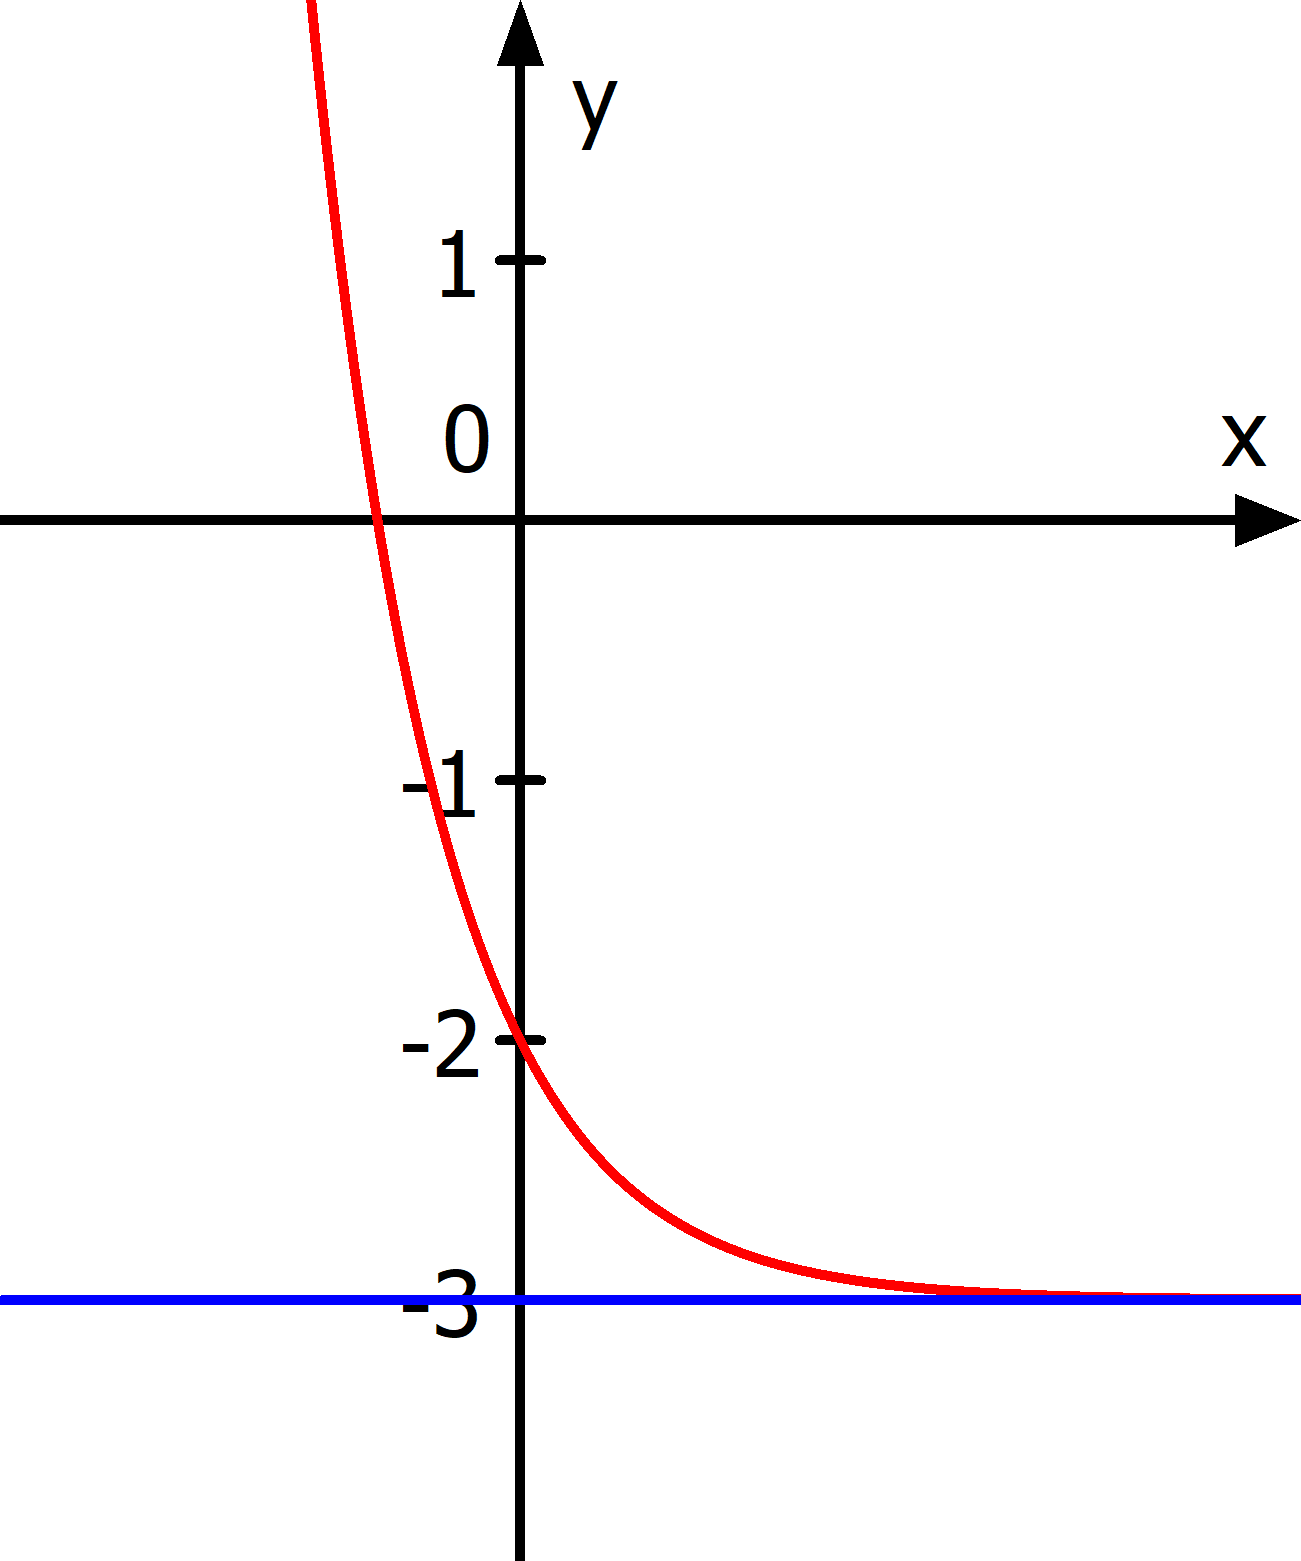
\includegraphics[width=.8\linewidth]{\eFkt/pics/A2a.png}
				\item \(f(x)=2e^{\frac{1}{2}x}+1\)

				Asymptote \(y=1\)

				y-Achsenabschnitt: \(f(0)=3\)

				Monoton wachsend

				\(f(x)\xrightarrow{\hphantom{\ }x\to-\infty\hphantom{\ }}1\)

				\(f(x)\xrightarrow{\hphantom{\ }x\to\infty\hphantom{\ }}\infty\)

				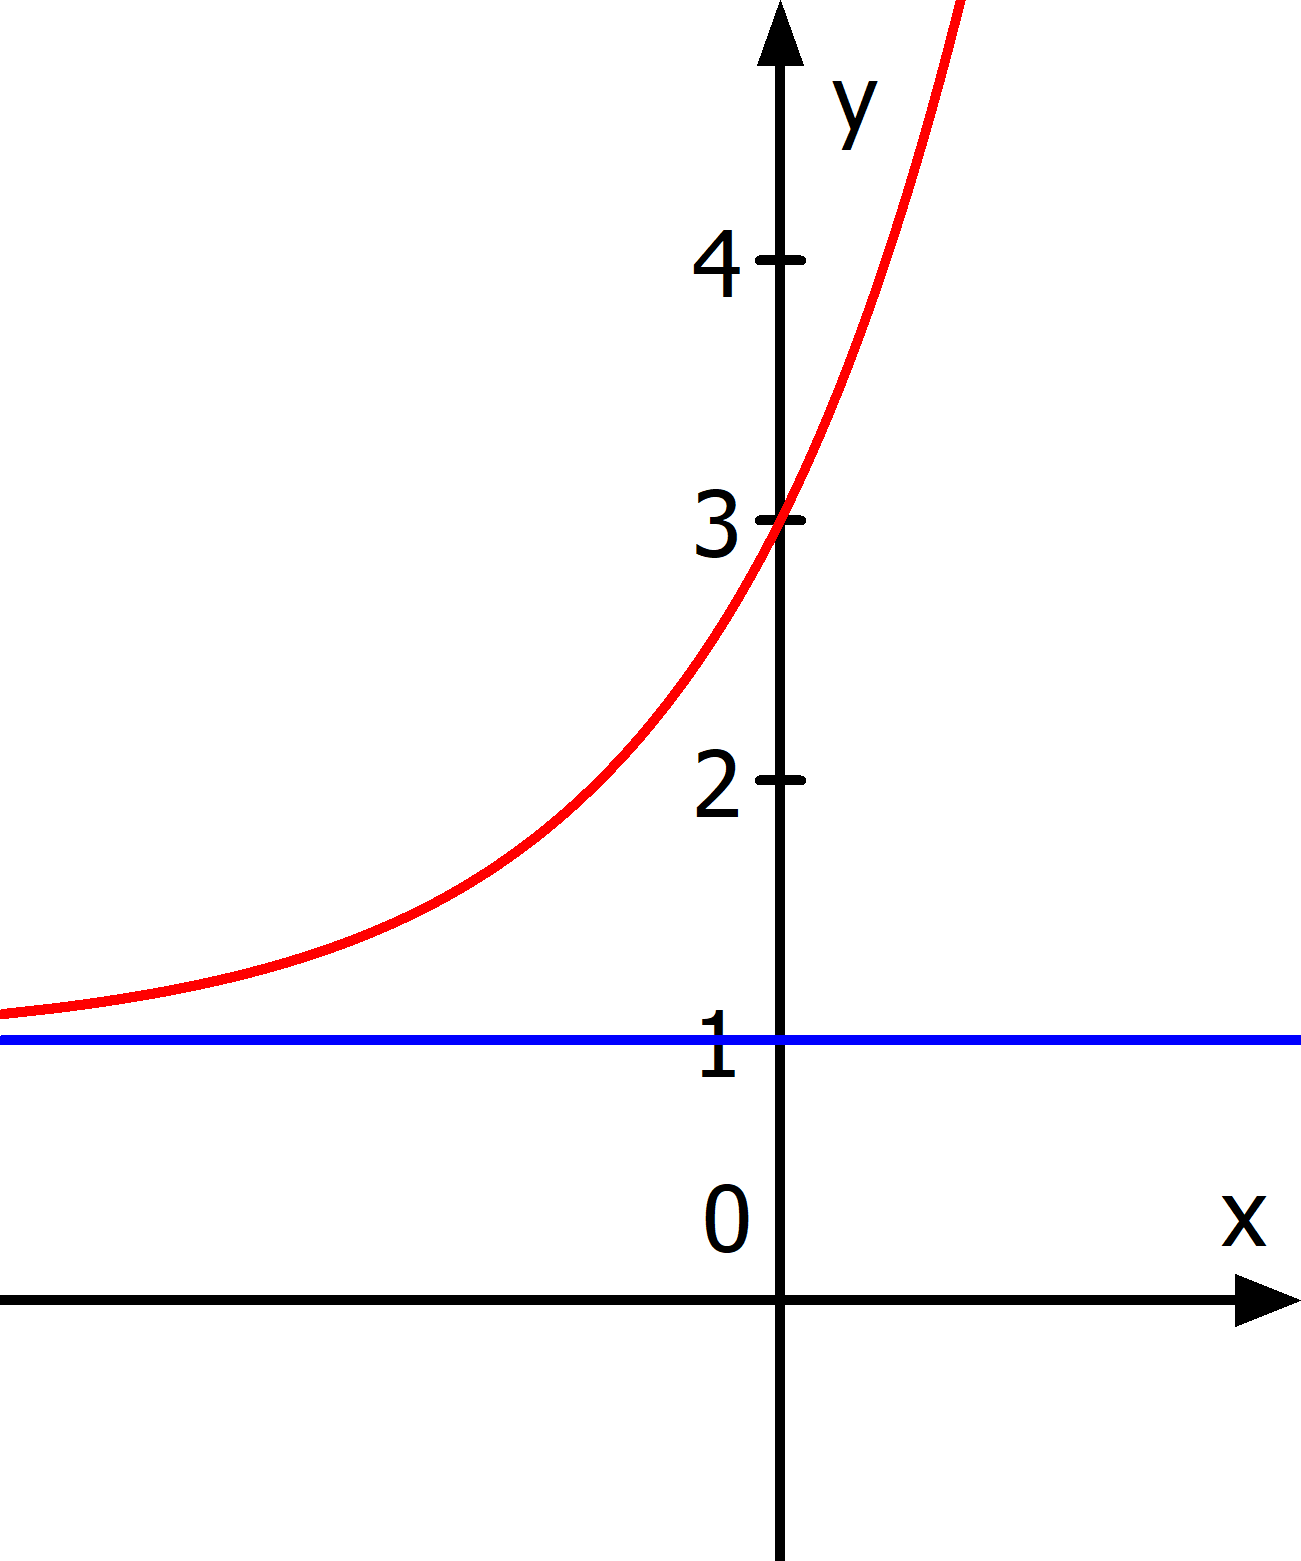
\includegraphics[width=.8\linewidth]{\eFkt/pics/A2b.png}
			\end{enumerate}
		\end{minipage}%
		\begin{minipage}{0.5\textwidth}
			\begin{enumerate}[label=\alph*)]
				\setcounter{enumi}{2}
				\item \(f(x)=-3e^{2x}+6\)

				Asymptote \(y=6\)

				y-Achsenabschnitt: \(f(0)=3\)

				Monoton fallend

				\(f(x)\xrightarrow{\hphantom{\ }x\to-\infty\hphantom{\ }}6\)

				\(f(x)\xrightarrow{\hphantom{\ }x\to\infty\hphantom{\ }}-\infty\)

				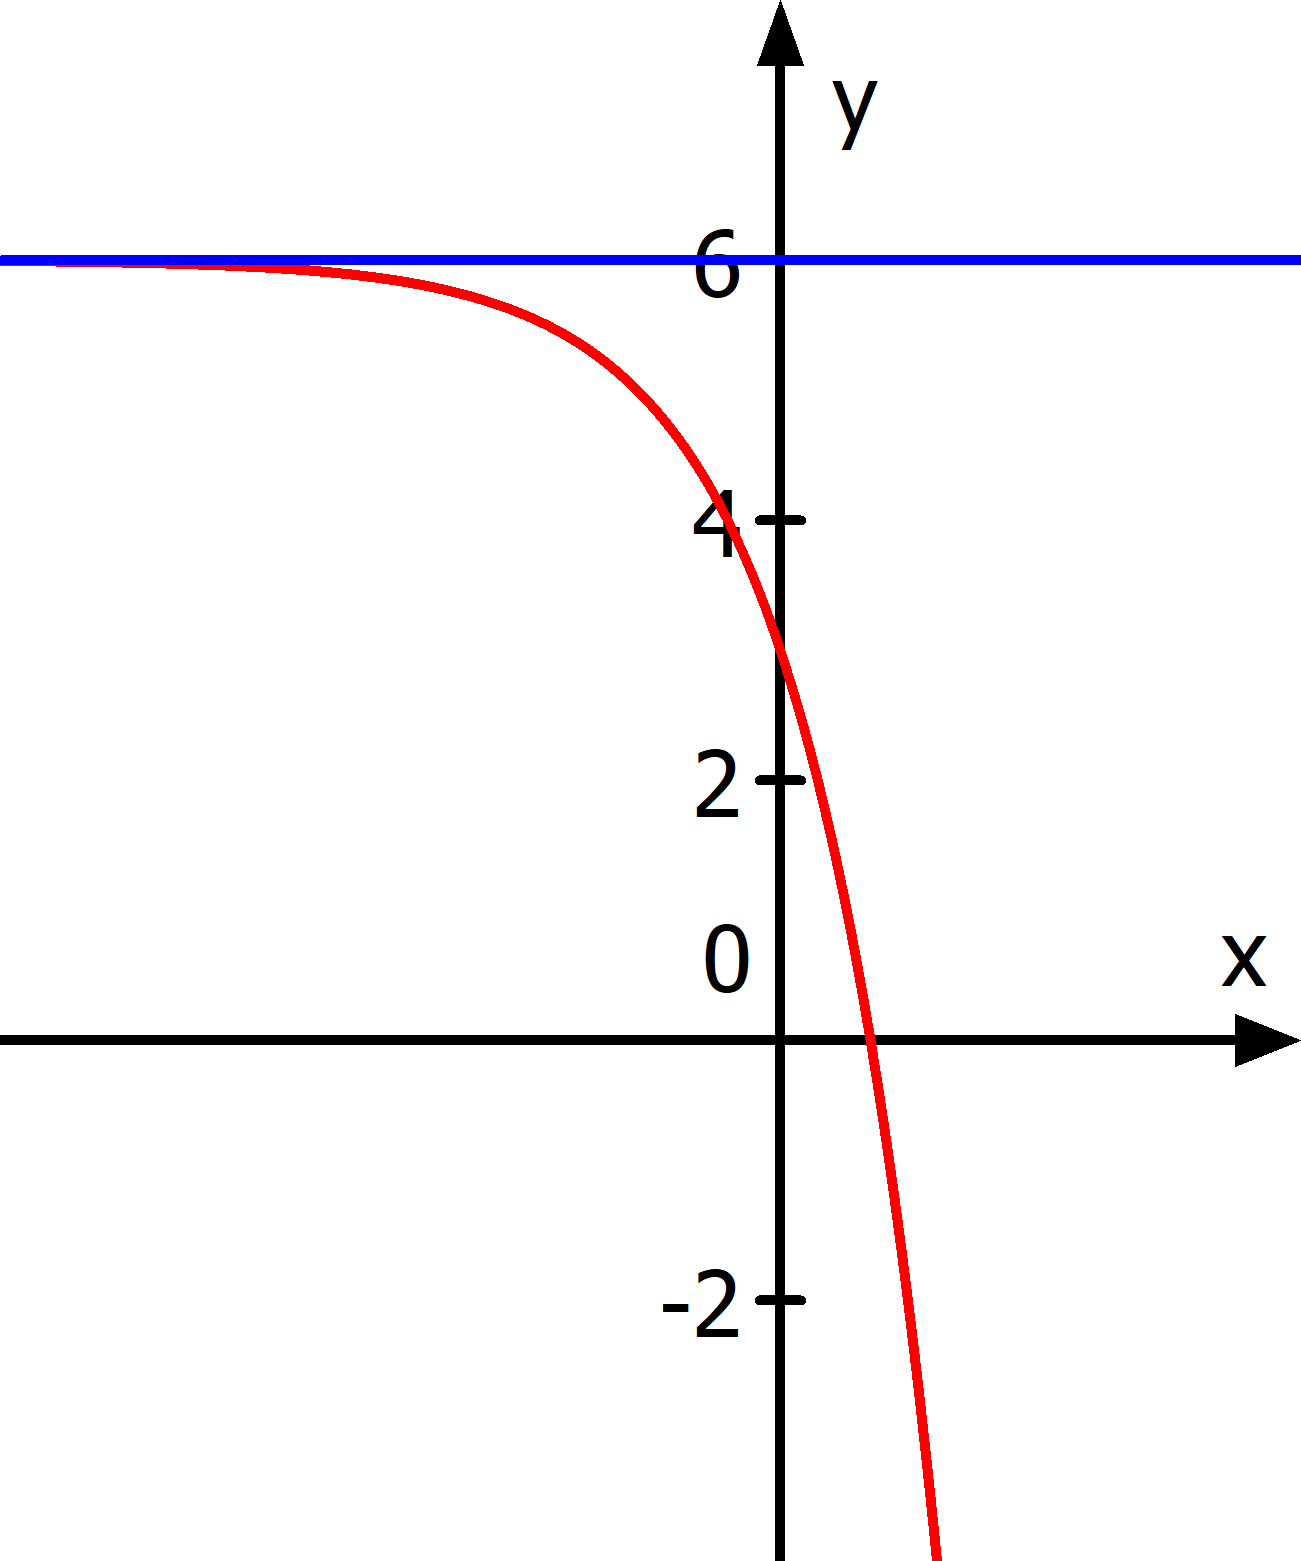
\includegraphics[width=.8\linewidth]{\eFkt/pics/A2c.png}
				\item \(f(x)=-2e^{-7x}-1\)

				Asymptote \(y=-1\)

				y-Achsenabschnitt: \(f(0)=-3\)

				Monoton wachsend

				\(f(x)\xrightarrow{\hphantom{\ }x\to-\infty\hphantom{\ }}-\infty\)

				\(f(x)\xrightarrow{\hphantom{\ }x\to\infty\hphantom{\ }}-1\)

				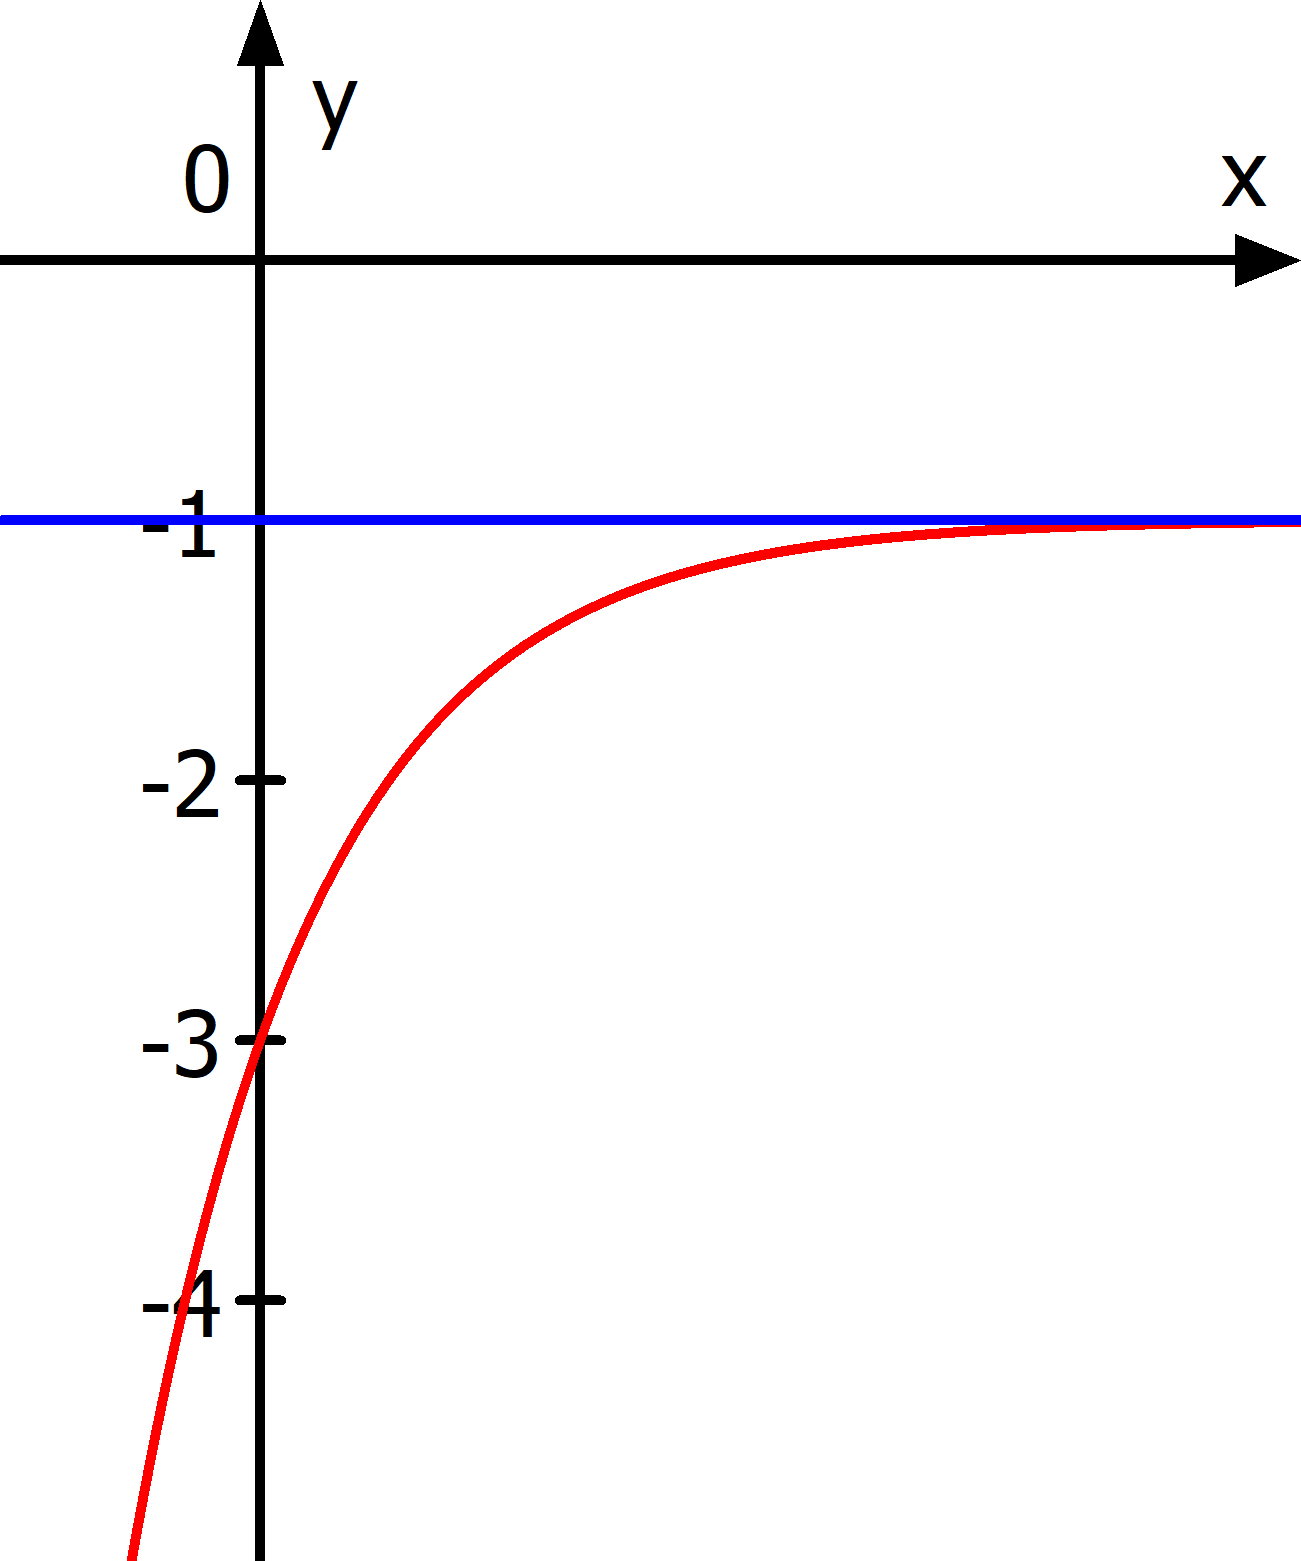
\includegraphics[width=.8\linewidth]{\eFkt/pics/A2d.png}
			\end{enumerate}
		\end{minipage}%
	\end{minipage}
	\newpage
	%%%%% e bis h
	\begin{minipage}{\textwidth}
		\begin{minipage}{0.5\textwidth}
			\begin{enumerate}[label=\alph*)]
				\setcounter{enumi}{4}
				\item \(f(x)=\frac{5}{2}e^{2x}-2\)

				Asymptote \(y=-2\)

				y-Achsenabschnitt: \(f(0)=\frac{1}{2}\)

				Monoton wachsend

				\(f(x)\xrightarrow{\hphantom{\ }x\to-\infty\hphantom{\ }}-2\)

				\(f(x)\xrightarrow{\hphantom{\ }x\to\infty\hphantom{\ }}\infty\)

				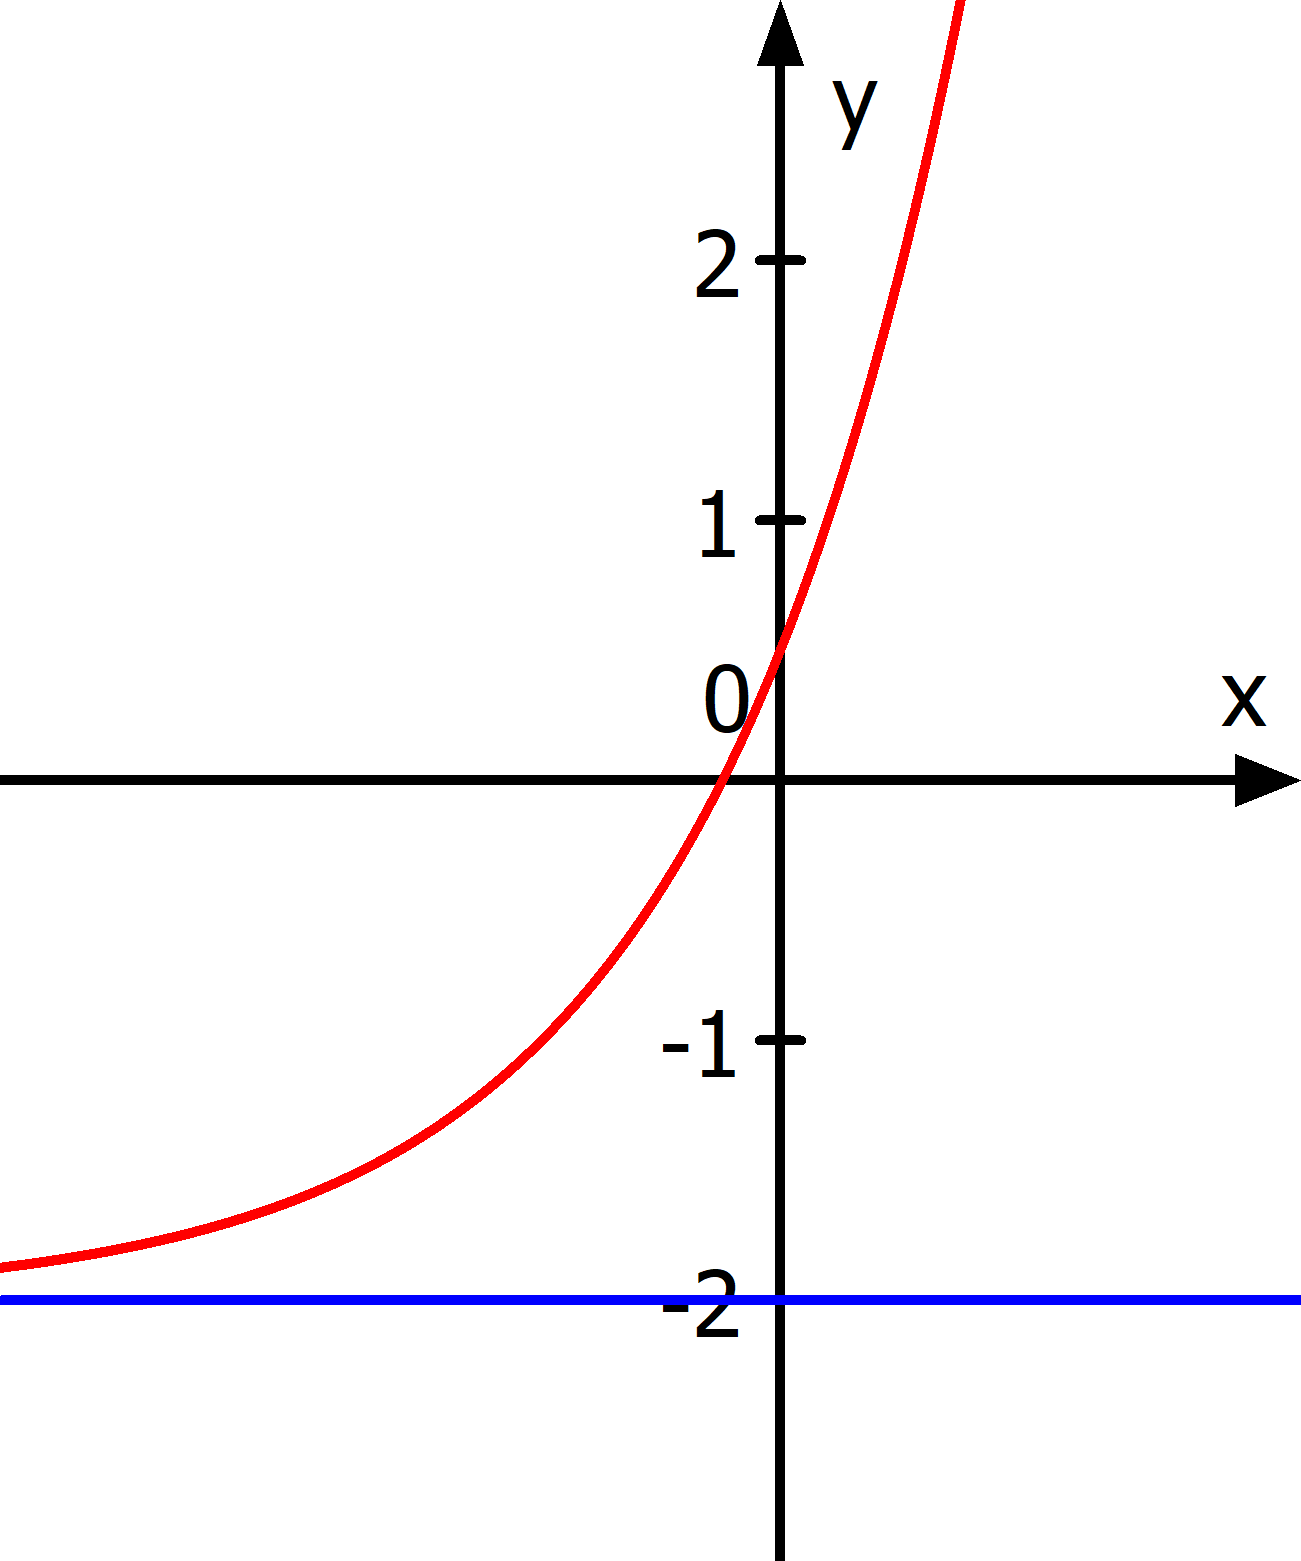
\includegraphics[width=.8\linewidth]{\eFkt/pics/A2e.png}
				\item \(f(x)=-8e^{3x}+8\)

				Asymptote \(y=8\)

				y-Achsenabschnitt: \(f(0)=0\)

				Monoton fallend

				\(f(x)\xrightarrow{\hphantom{\ }x\to-\infty\hphantom{\ }}8\)

				\(f(x)\xrightarrow{\hphantom{\ }x\to\infty\hphantom{\ }}-\infty\)

				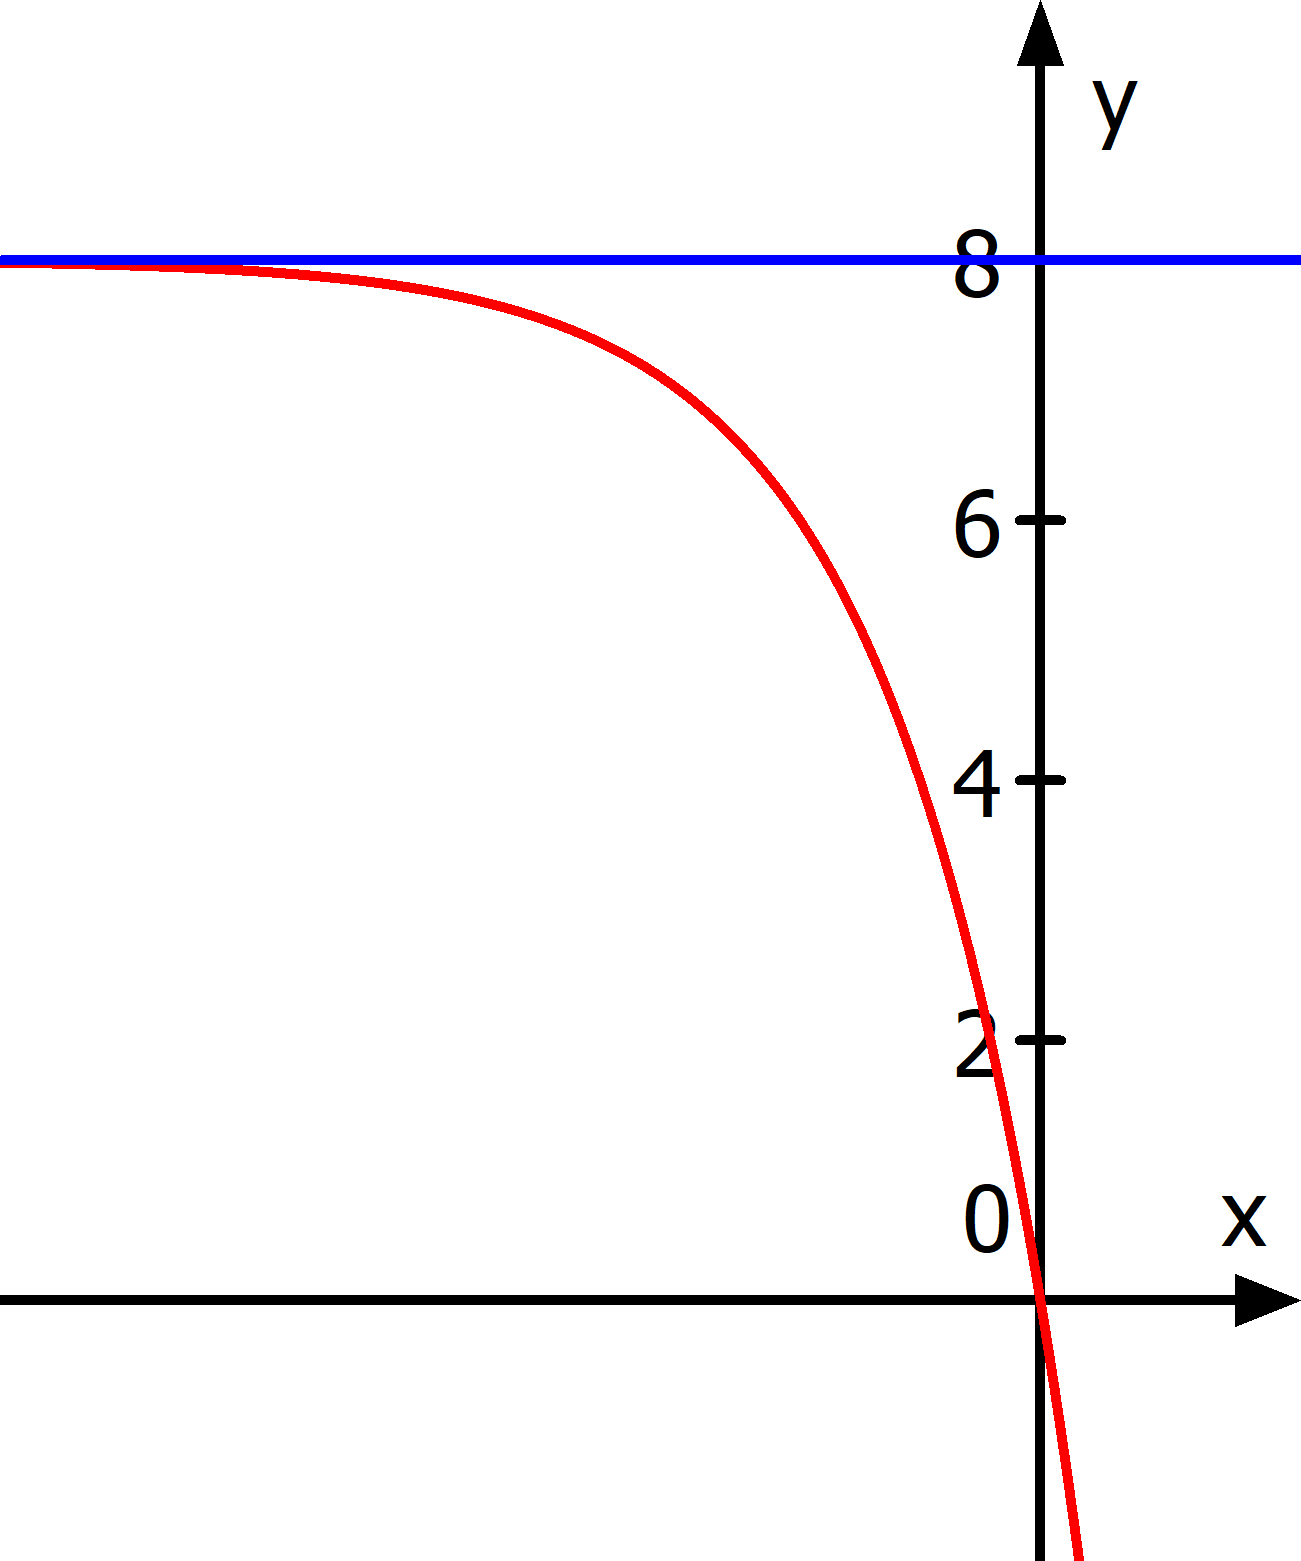
\includegraphics[width=.8\linewidth]{\eFkt/pics/A2f.png}
			\end{enumerate}
		\end{minipage}%
		\begin{minipage}{0.5\textwidth}
			\begin{enumerate}[label=\alph*)]
				\setcounter{enumi}{6}
				\item \(f(x)=2e^{-\frac{3}{8}x}-5\)

				Asymptote \(y=-5\)

				y-Achsenabschnitt: \(f(0)=-3\)

				Monoton fallend

				\(f(x)\xrightarrow{\hphantom{\ }x\to-\infty\hphantom{\ }}\infty\)

				\(f(x)\xrightarrow{\hphantom{\ }x\to\infty\hphantom{\ }}-5\)

				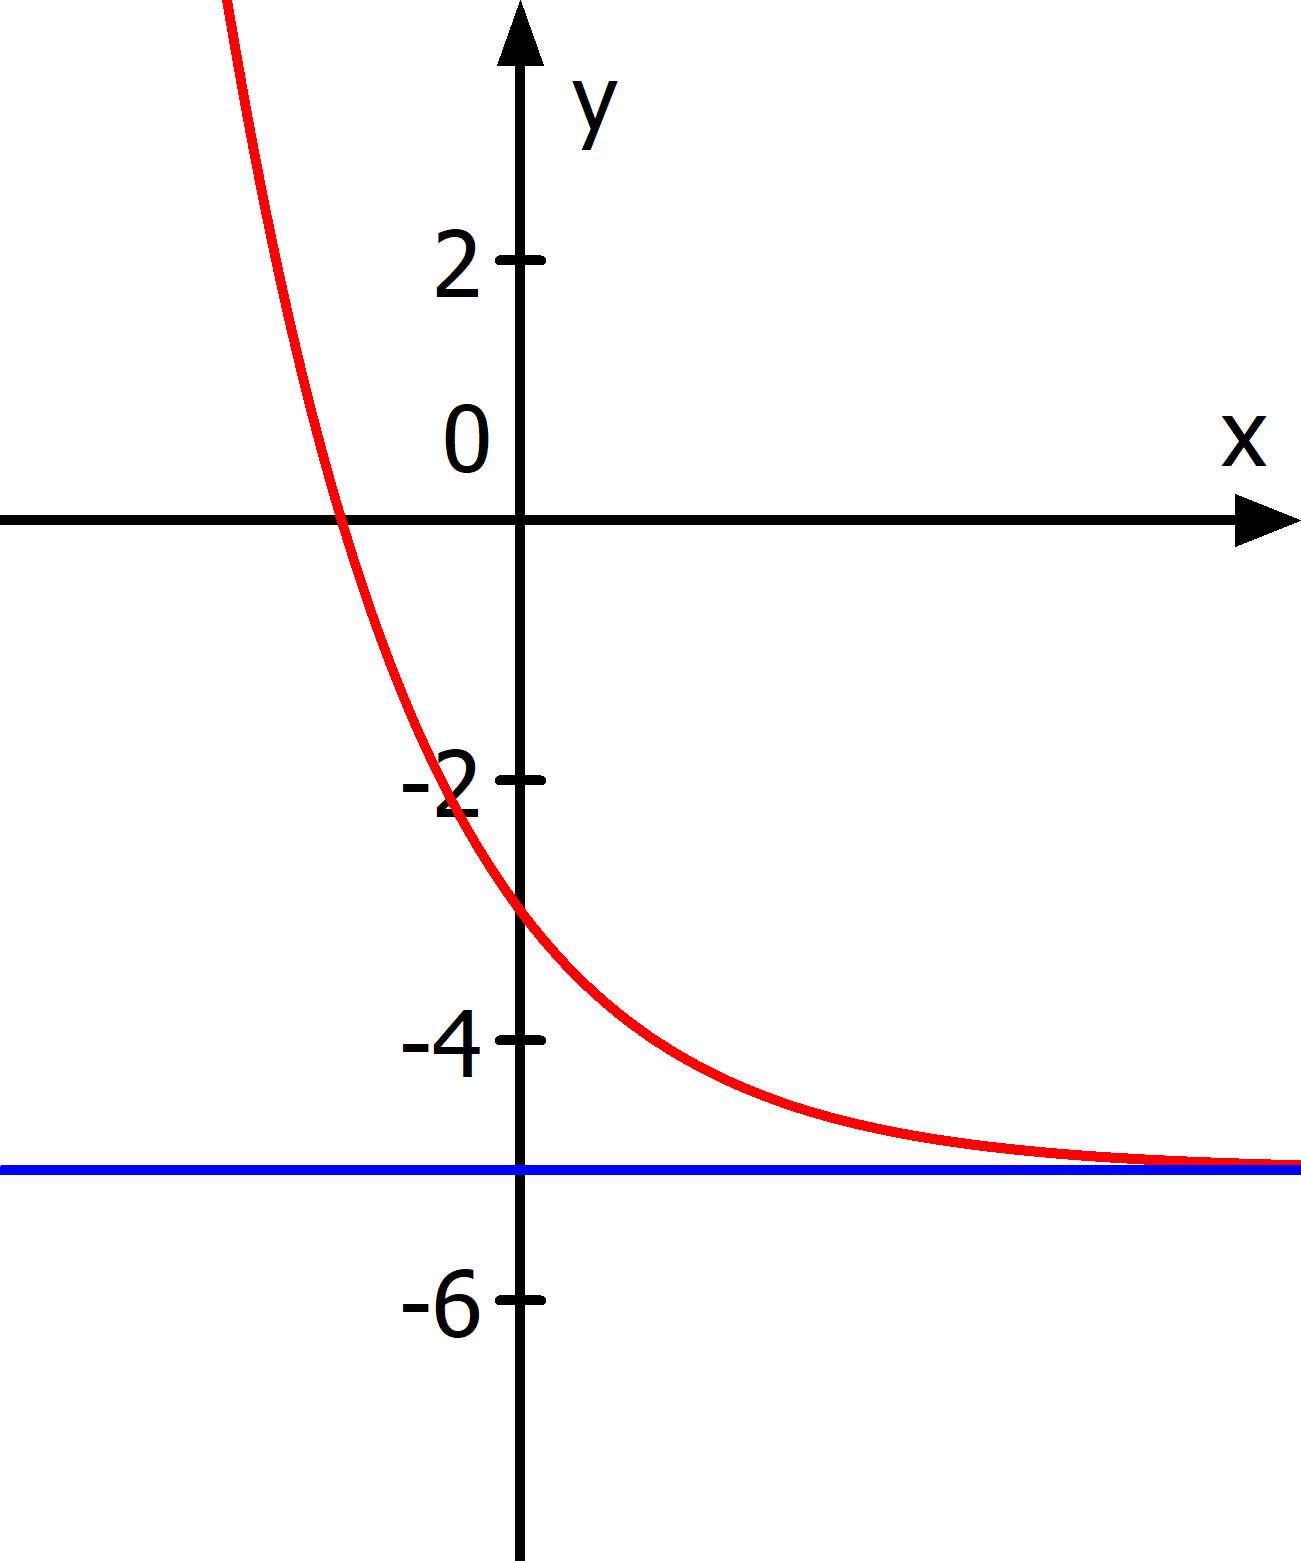
\includegraphics[width=.8\linewidth]{\eFkt/pics/A2g.png}
				\item \(f(x)=-\frac{3}{2}e^{0,2x}+2\)

				Asymptote \(y=2\)

				y-Achsenabschnitt: \(f(0)=\frac{1}{2}\)

				Monoton fallend

				\(f(x)\xrightarrow{\hphantom{\ }x\to-\infty\hphantom{\ }}2\)

				\(f(x)\xrightarrow{\hphantom{\ }x\to\infty\hphantom{\ }}-\infty\)

				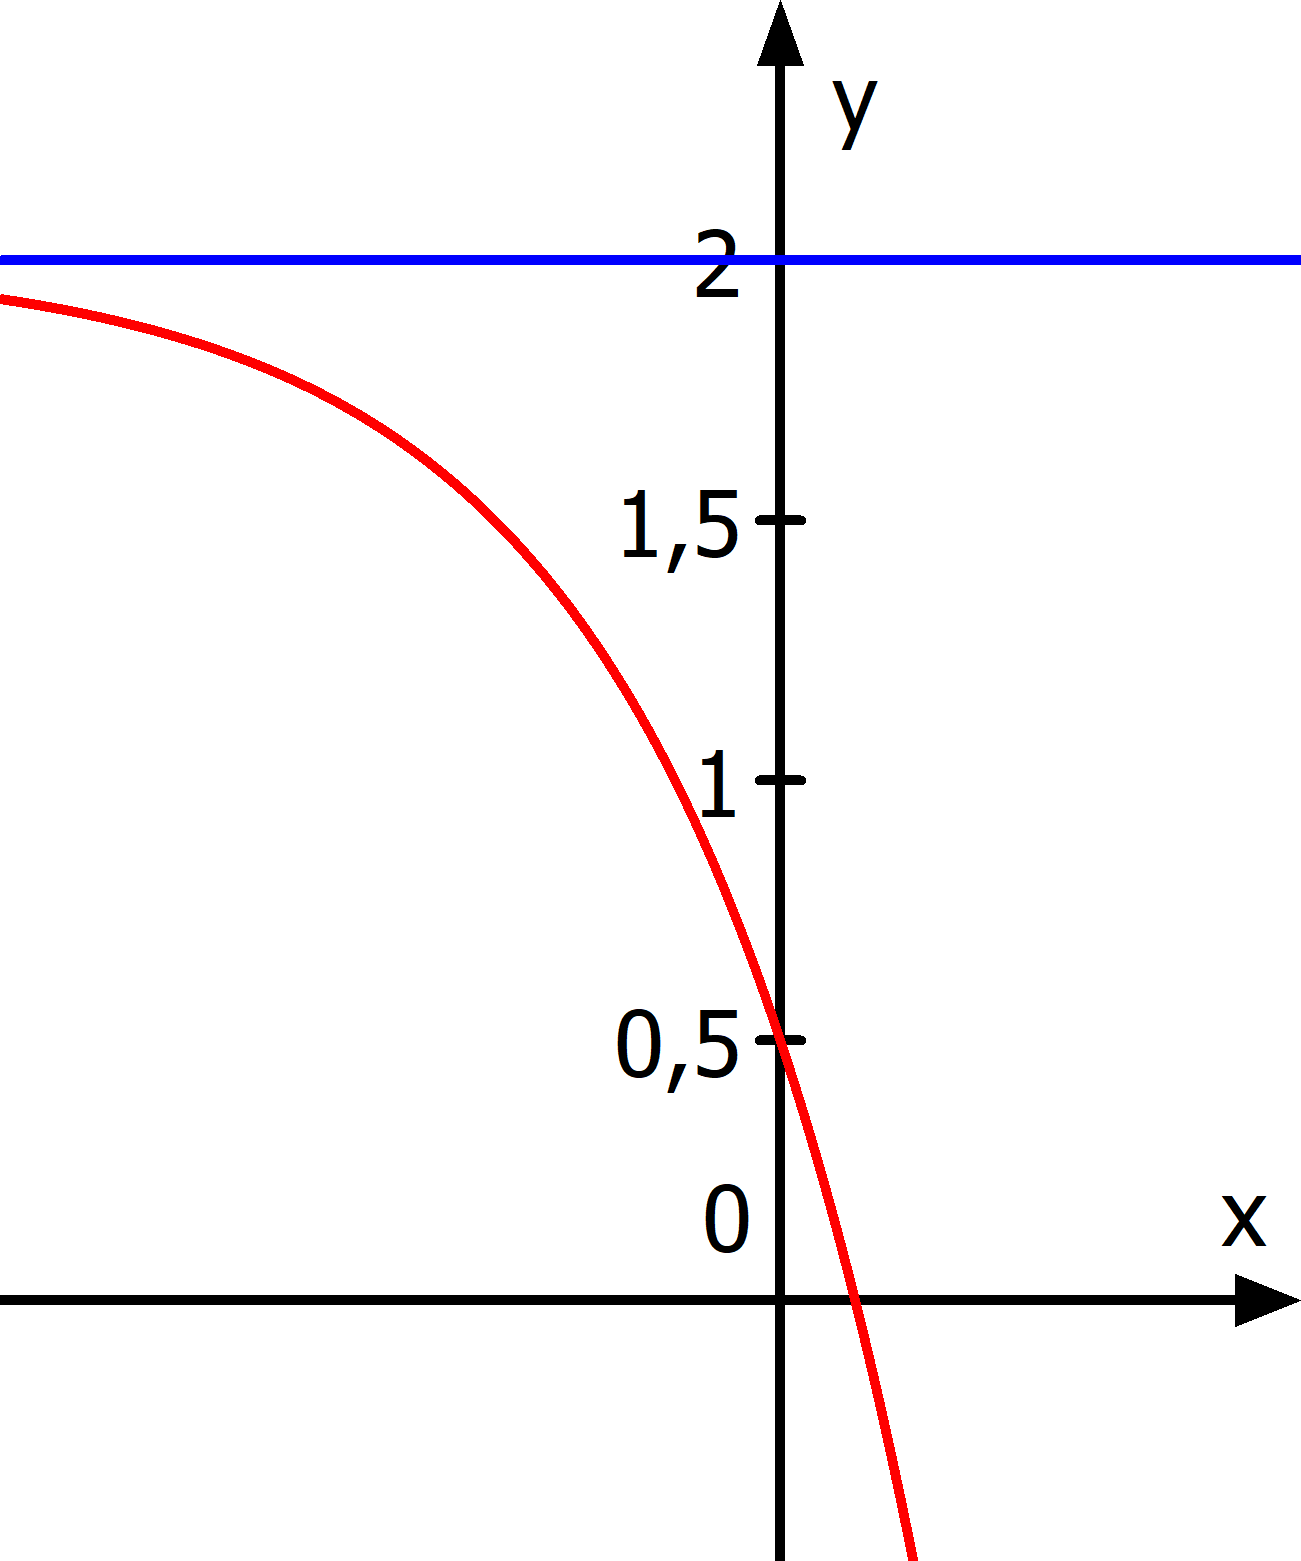
\includegraphics[width=.8\linewidth]{\eFkt/pics/A2h.png}
			\end{enumerate}
		\end{minipage}%
	\end{minipage}
	\newpage
	%%%%% i bis l
	\begin{minipage}{\textwidth}
		\begin{minipage}{0.5\textwidth}
			\begin{enumerate}[label=\alph*)]
				\setcounter{enumi}{8}
				\item \(f(x)=-5e^{-3,5x}+5\)

				Asymptote \(y=5\)

				y-Achsenabschnitt: \(f(0)=0\)

				Monoton wachsend

				\(f(x)\xrightarrow{\hphantom{\ }x\to-\infty\hphantom{\ }}-\infty\)

				\(f(x)\xrightarrow{\hphantom{\ }x\to\infty\hphantom{\ }}5\)

				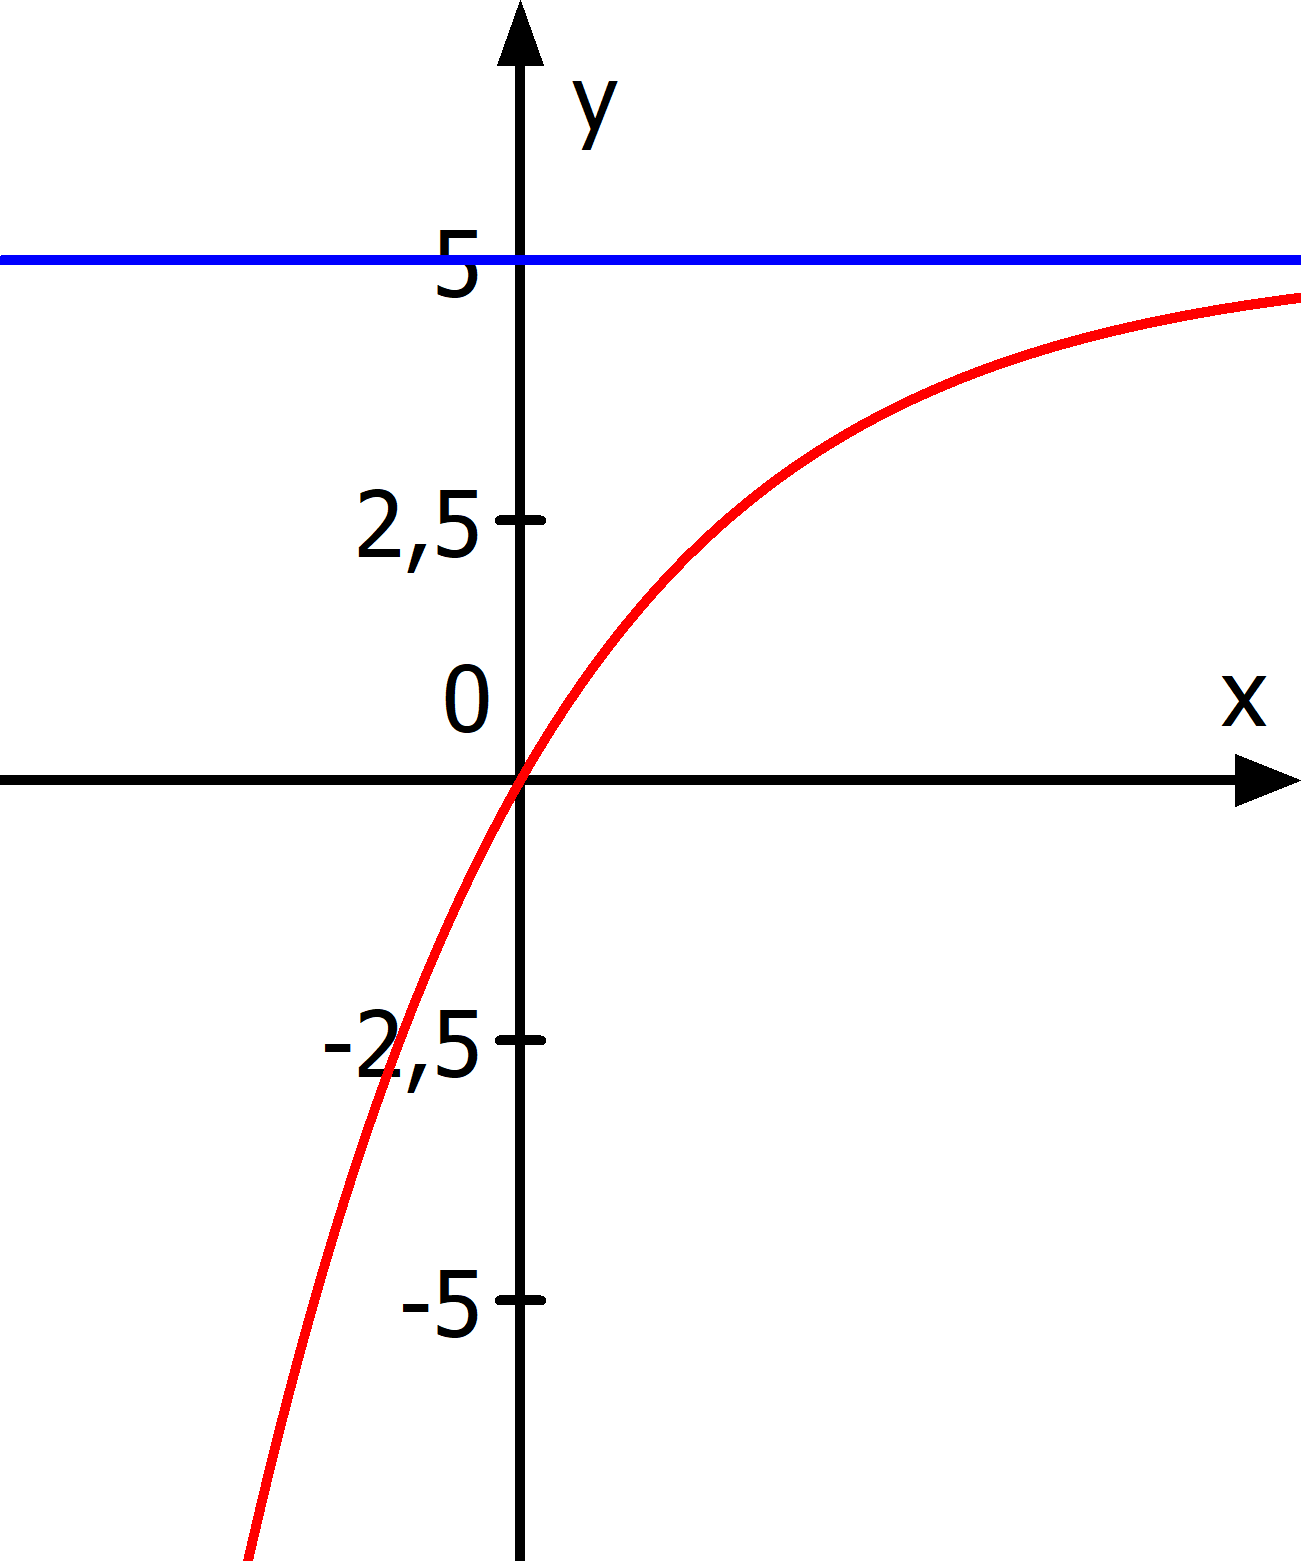
\includegraphics[width=.8\linewidth]{\eFkt/pics/A2i.png}
				\item \(f(x)=-8e^{0,3x}+6\)

				Asymptote \(y=6\)

				y-Achsenabschnitt: \(f(0)=-2\)

				Monoton fallend

				\(f(x)\xrightarrow{\hphantom{\ }x\to-\infty\hphantom{\ }}6\)

				\(f(x)\xrightarrow{\hphantom{\ }x\to\infty\hphantom{\ }}-\infty\)

				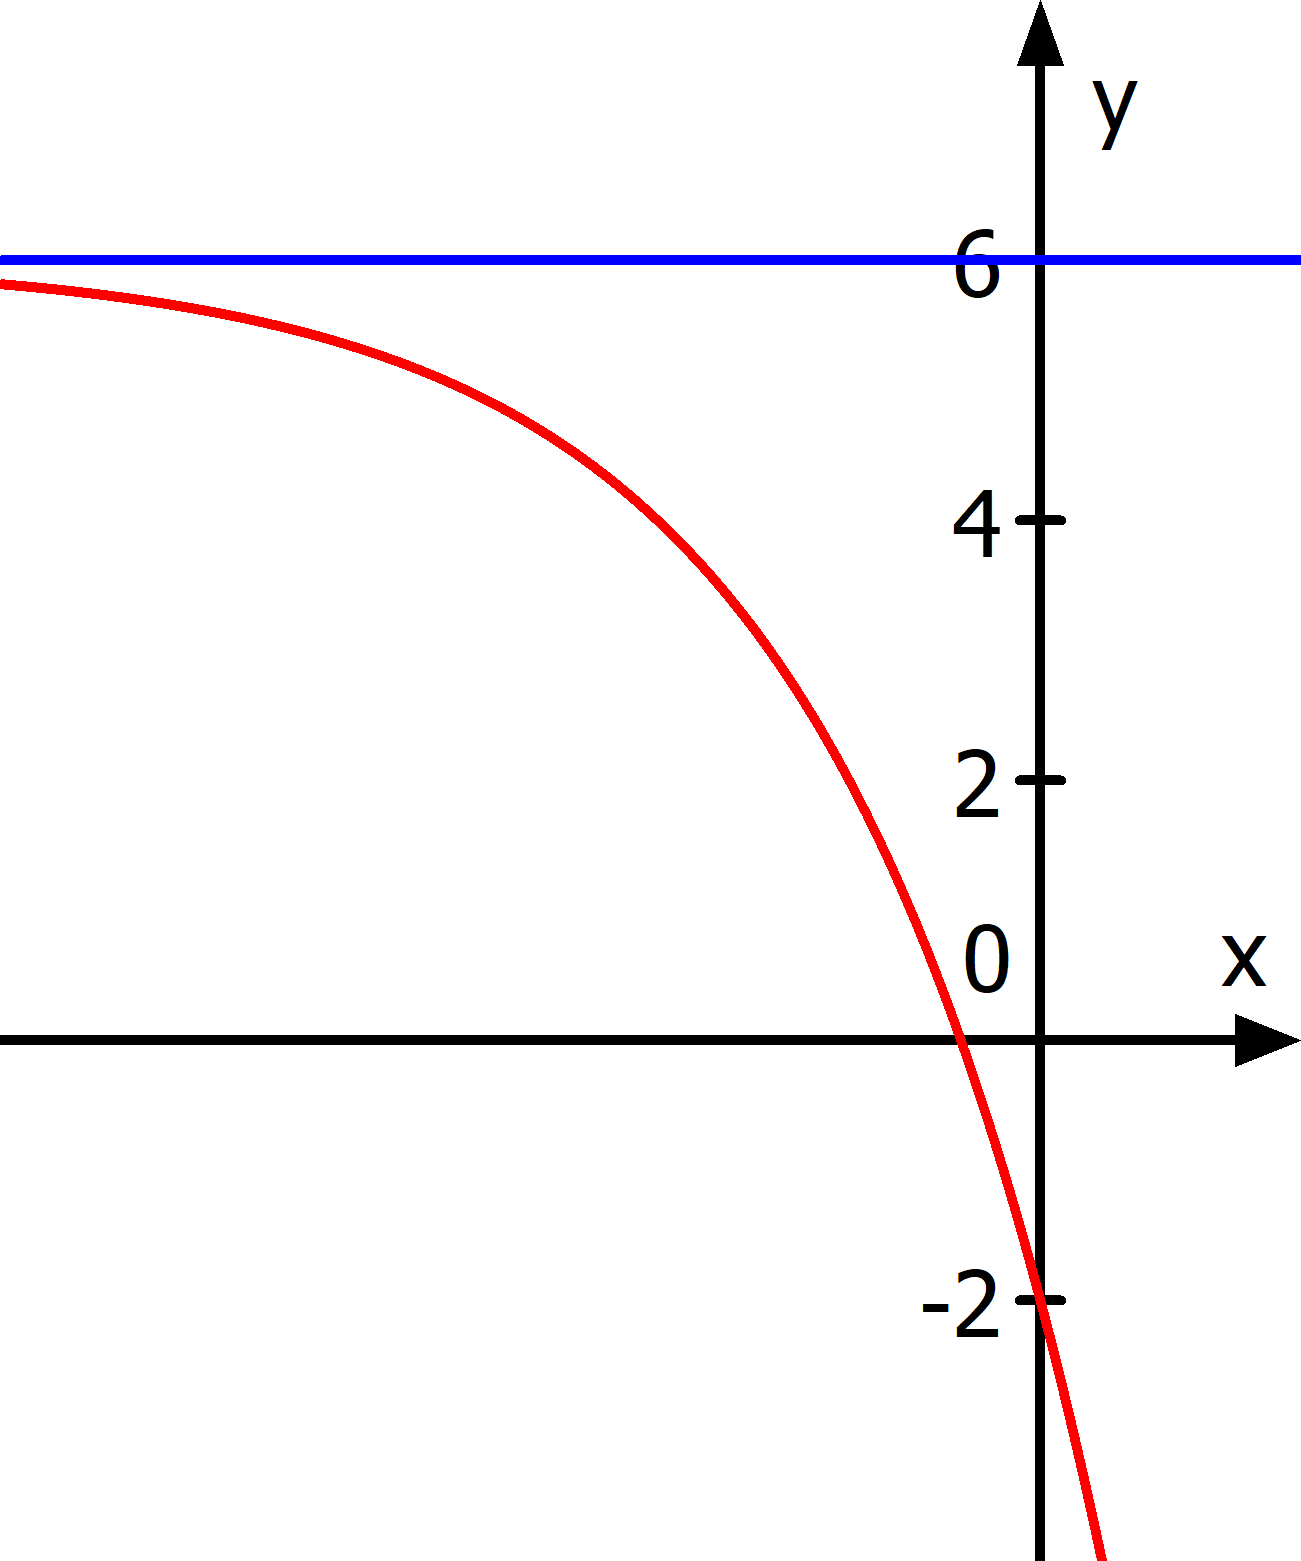
\includegraphics[width=.8\linewidth]{\eFkt/pics/A2j.png}
			\end{enumerate}
		\end{minipage}%
		\begin{minipage}{0.5\textwidth}
			\begin{enumerate}[label=\alph*)]
				\setcounter{enumi}{10}
				\item \(f(x)=2e^{-2x}+2\)

				Asymptote \(y=2\)

				y-Achsenabschnitt: \(f(0)=4\)

				Monoton fallend

				\(f(x)\xrightarrow{\hphantom{\ }x\to-\infty\hphantom{\ }}\infty\)

				\(f(x)\xrightarrow{\hphantom{\ }x\to\infty\hphantom{\ }}2\)

				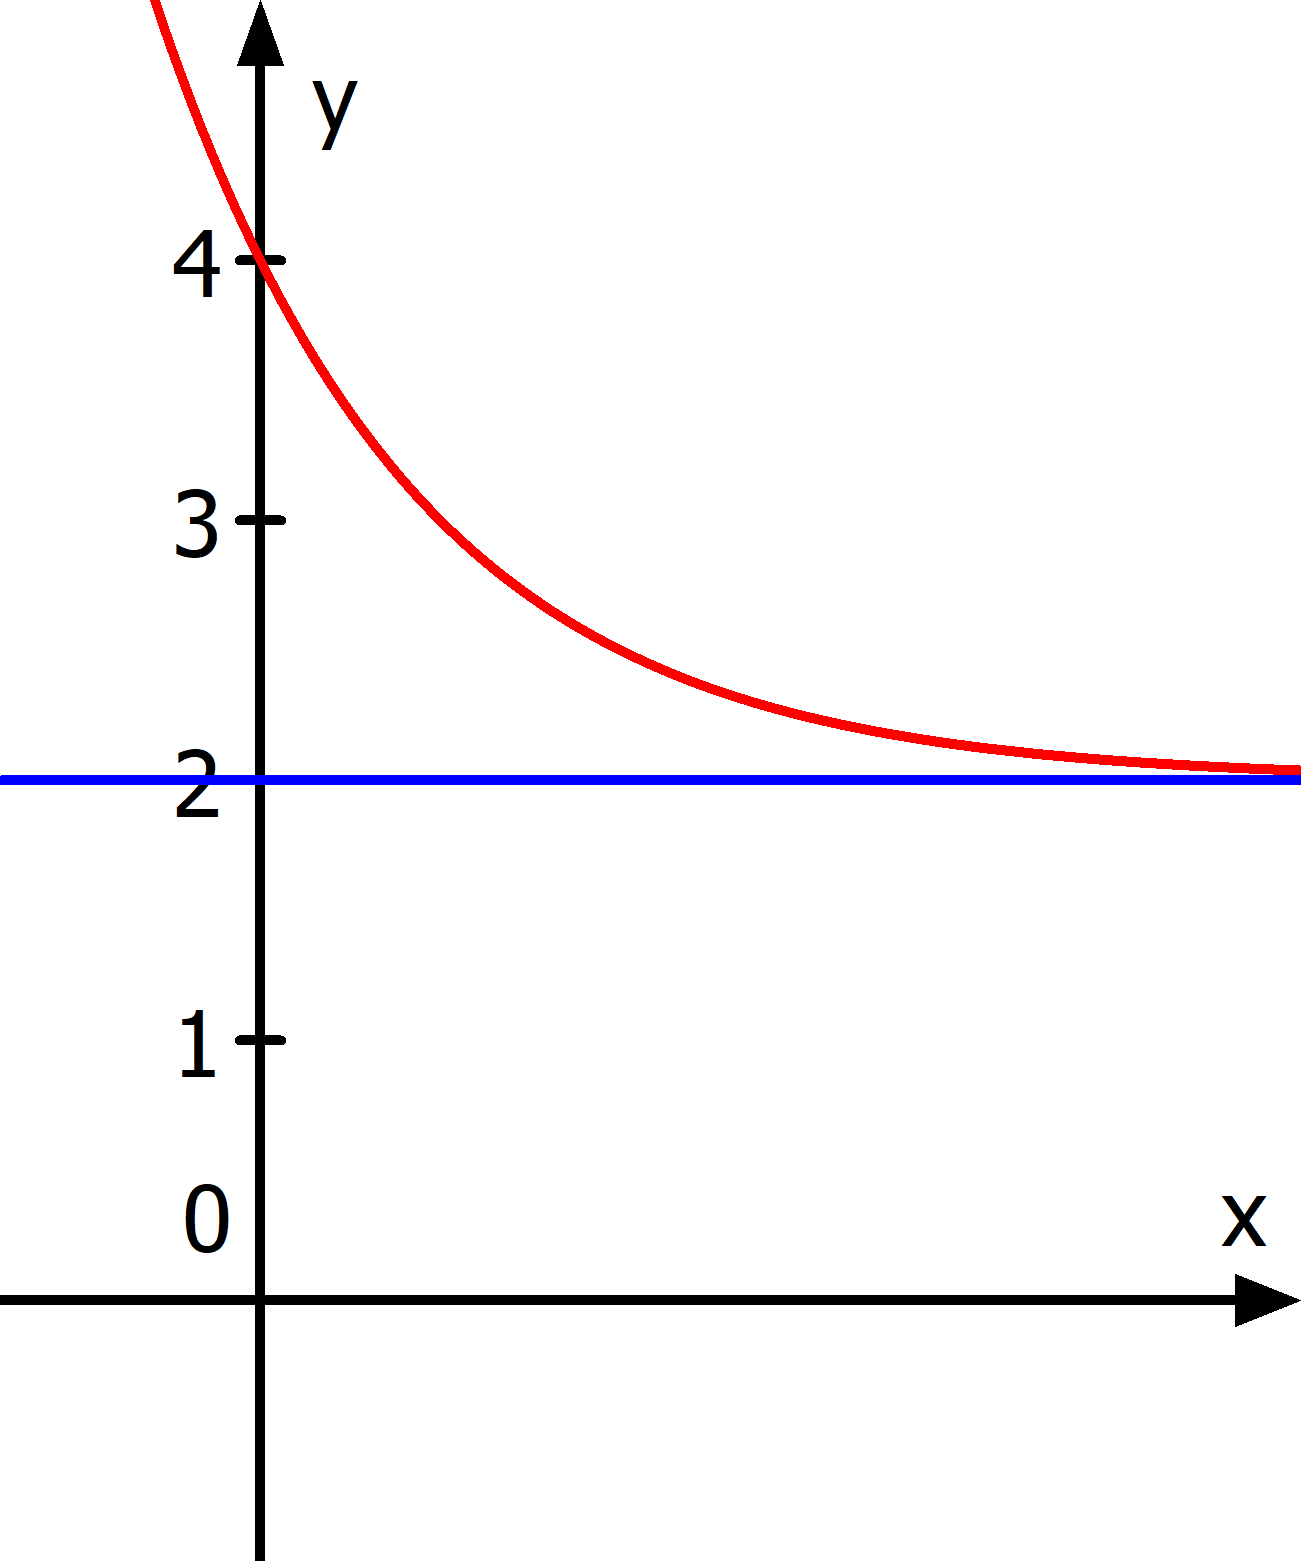
\includegraphics[width=.8\linewidth]{\eFkt/pics/A2k.png}
				\item \(f(x)=-6+4e^{-7x}\)

				Asymptote \(y=-6\)

				y-Achsenabschnitt: \(f(0)=-2\)

				Monoton fallend

				\(f(x)\xrightarrow{\hphantom{\ }x\to-\infty\hphantom{\ }}\infty\)

				\(f(x)\xrightarrow{\hphantom{\ }x\to\infty\hphantom{\ }}-6\)

				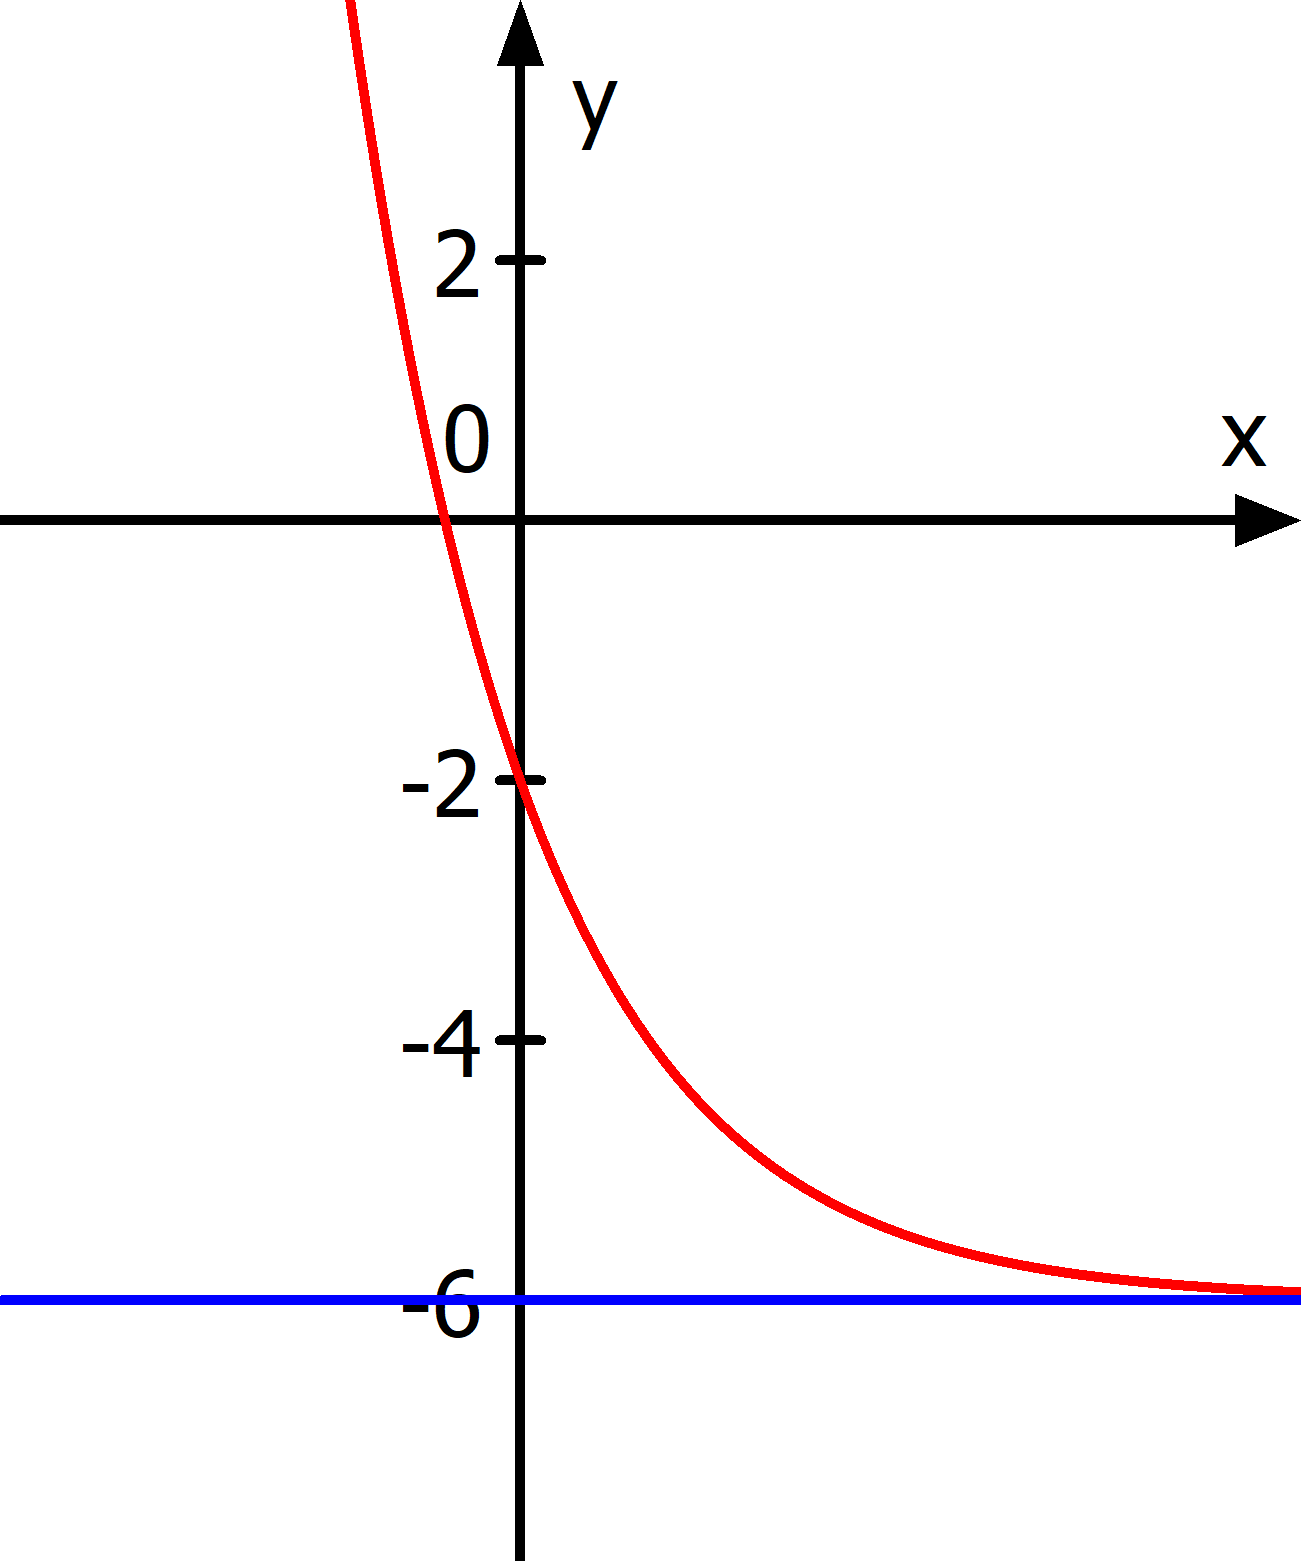
\includegraphics[width=.8\linewidth]{\eFkt/pics/A2l.png}
			\end{enumerate}
		\end{minipage}%
	\end{minipage}
	\newpage
	%%%%% m bis p
	\begin{minipage}{\textwidth}
		\begin{minipage}{0.5\textwidth}
			\begin{enumerate}[label=\alph*)]
				\setcounter{enumi}{12}
				\item \(f(x)=8-5e^{x}\)

				Asymptote \(y=8\)

				y-Achsenabschnitt: \(f(0)=3\)

				Monoton fallend

				\(f(x)\xrightarrow{\hphantom{\ }x\to-\infty\hphantom{\ }}8\)

				\(f(x)\xrightarrow{\hphantom{\ }x\to\infty\hphantom{\ }}-\infty\)

				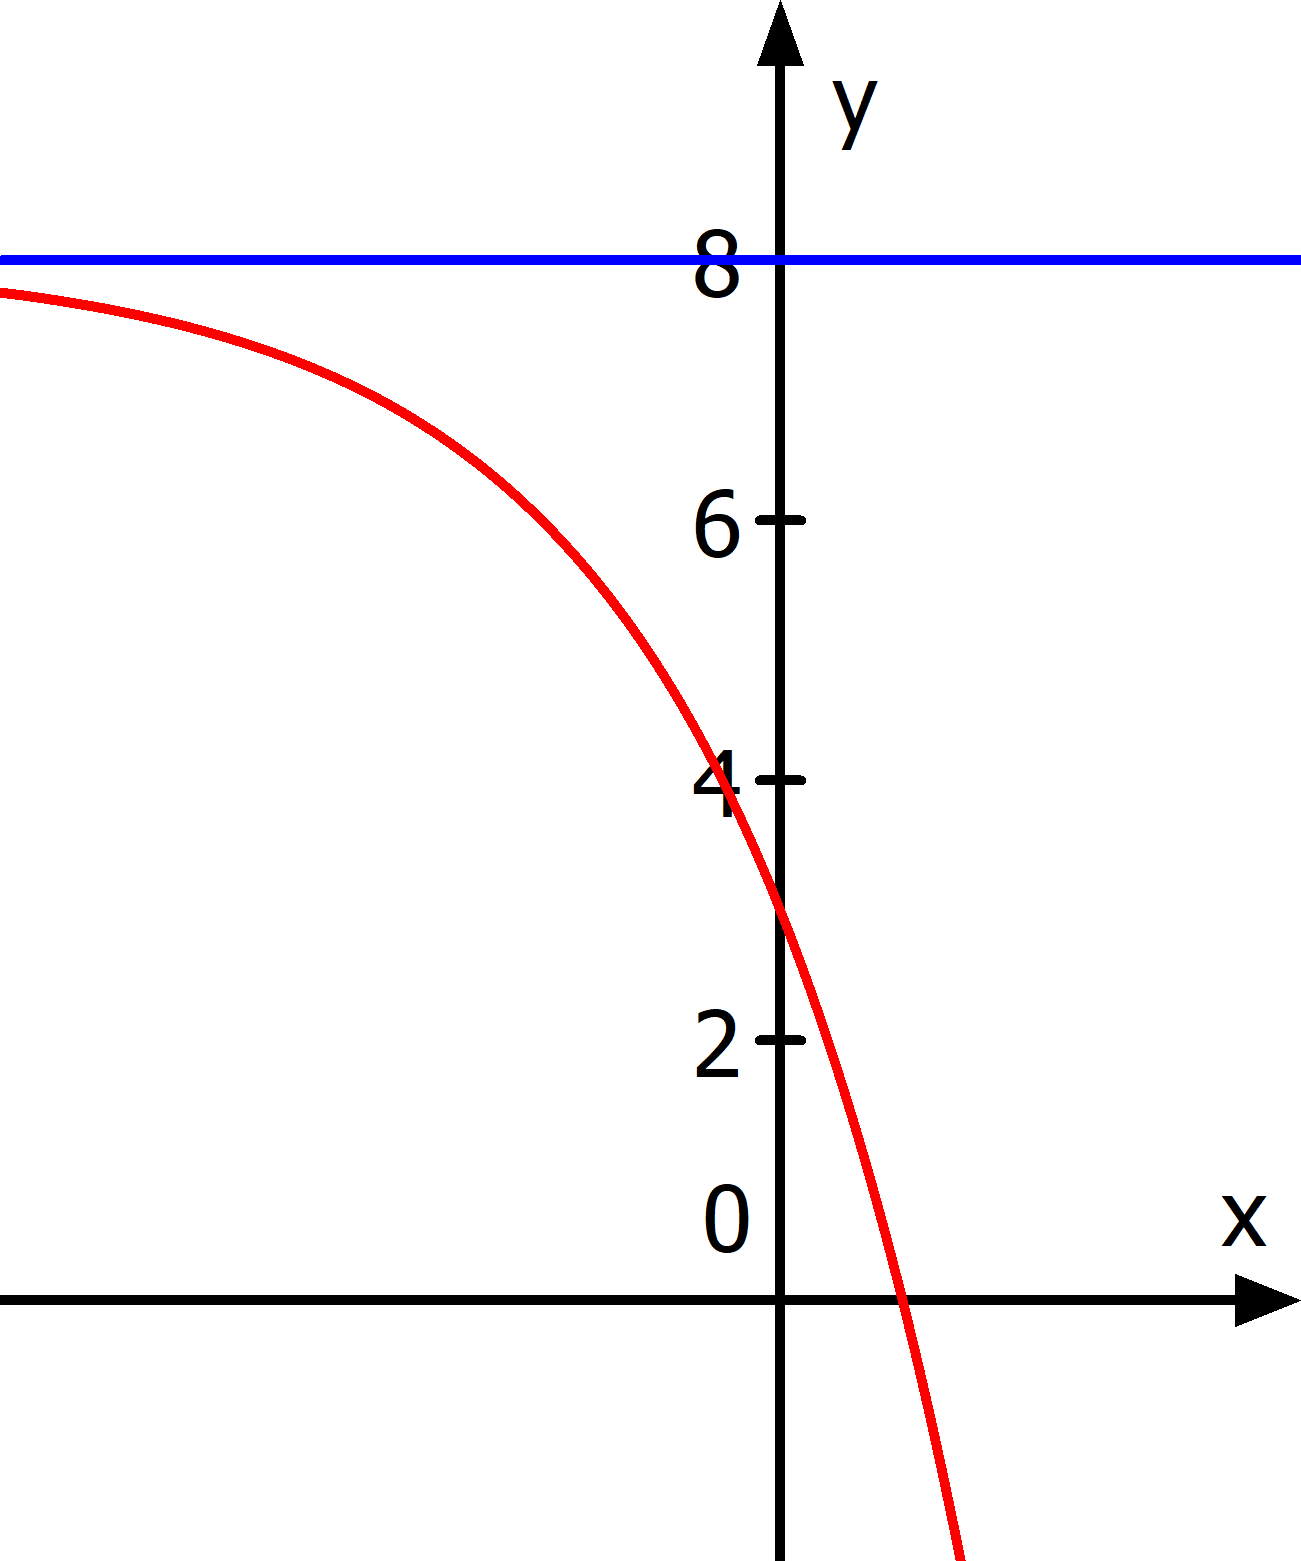
\includegraphics[width=.8\linewidth]{\eFkt/pics/A2m.png}
				\item \(f(x)=-4e^{-2x}-2\)

				Asymptote \(y=-2\)

				y-Achsenabschnitt: \(f(0)=-6\)

				Monoton wachsend

				\(f(x)\xrightarrow{\hphantom{\ }x\to-\infty\hphantom{\ }}-\infty\)

				\(f(x)\xrightarrow{\hphantom{\ }x\to\infty\hphantom{\ }}-2\)

				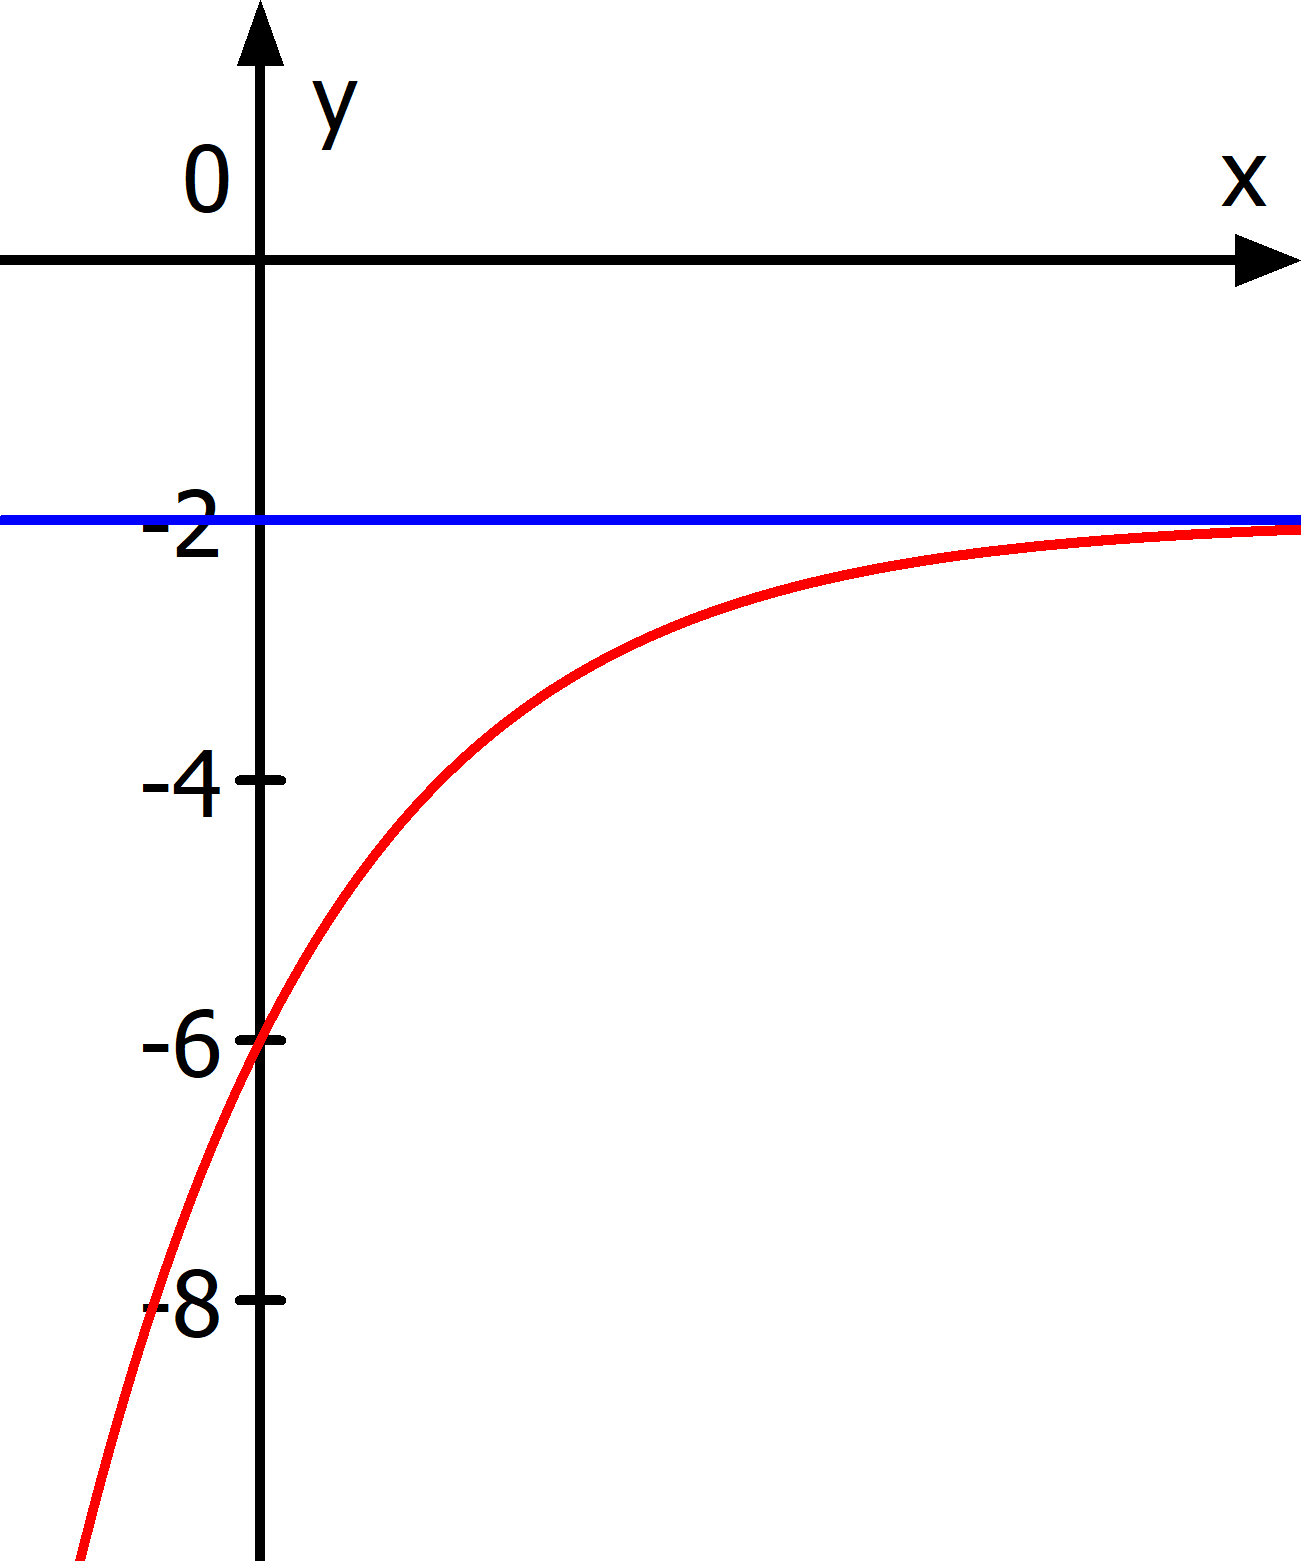
\includegraphics[width=.8\linewidth]{\eFkt/pics/A2n.png}
			\end{enumerate}
		\end{minipage}%
		\begin{minipage}{0.5\textwidth}
			\begin{enumerate}[label=\alph*)]
				\setcounter{enumi}{14}
				\item \(f(x)=2e^{-3x}+4\)

				Asymptote \(y=4\)

				y-Achsenabschnitt: \(f(0)=6\)

				Monoton fallend

				\(f(x)\xrightarrow{\hphantom{\ }x\to-\infty\hphantom{\ }}\infty\)

				\(f(x)\xrightarrow{\hphantom{\ }x\to\infty\hphantom{\ }}4\)

				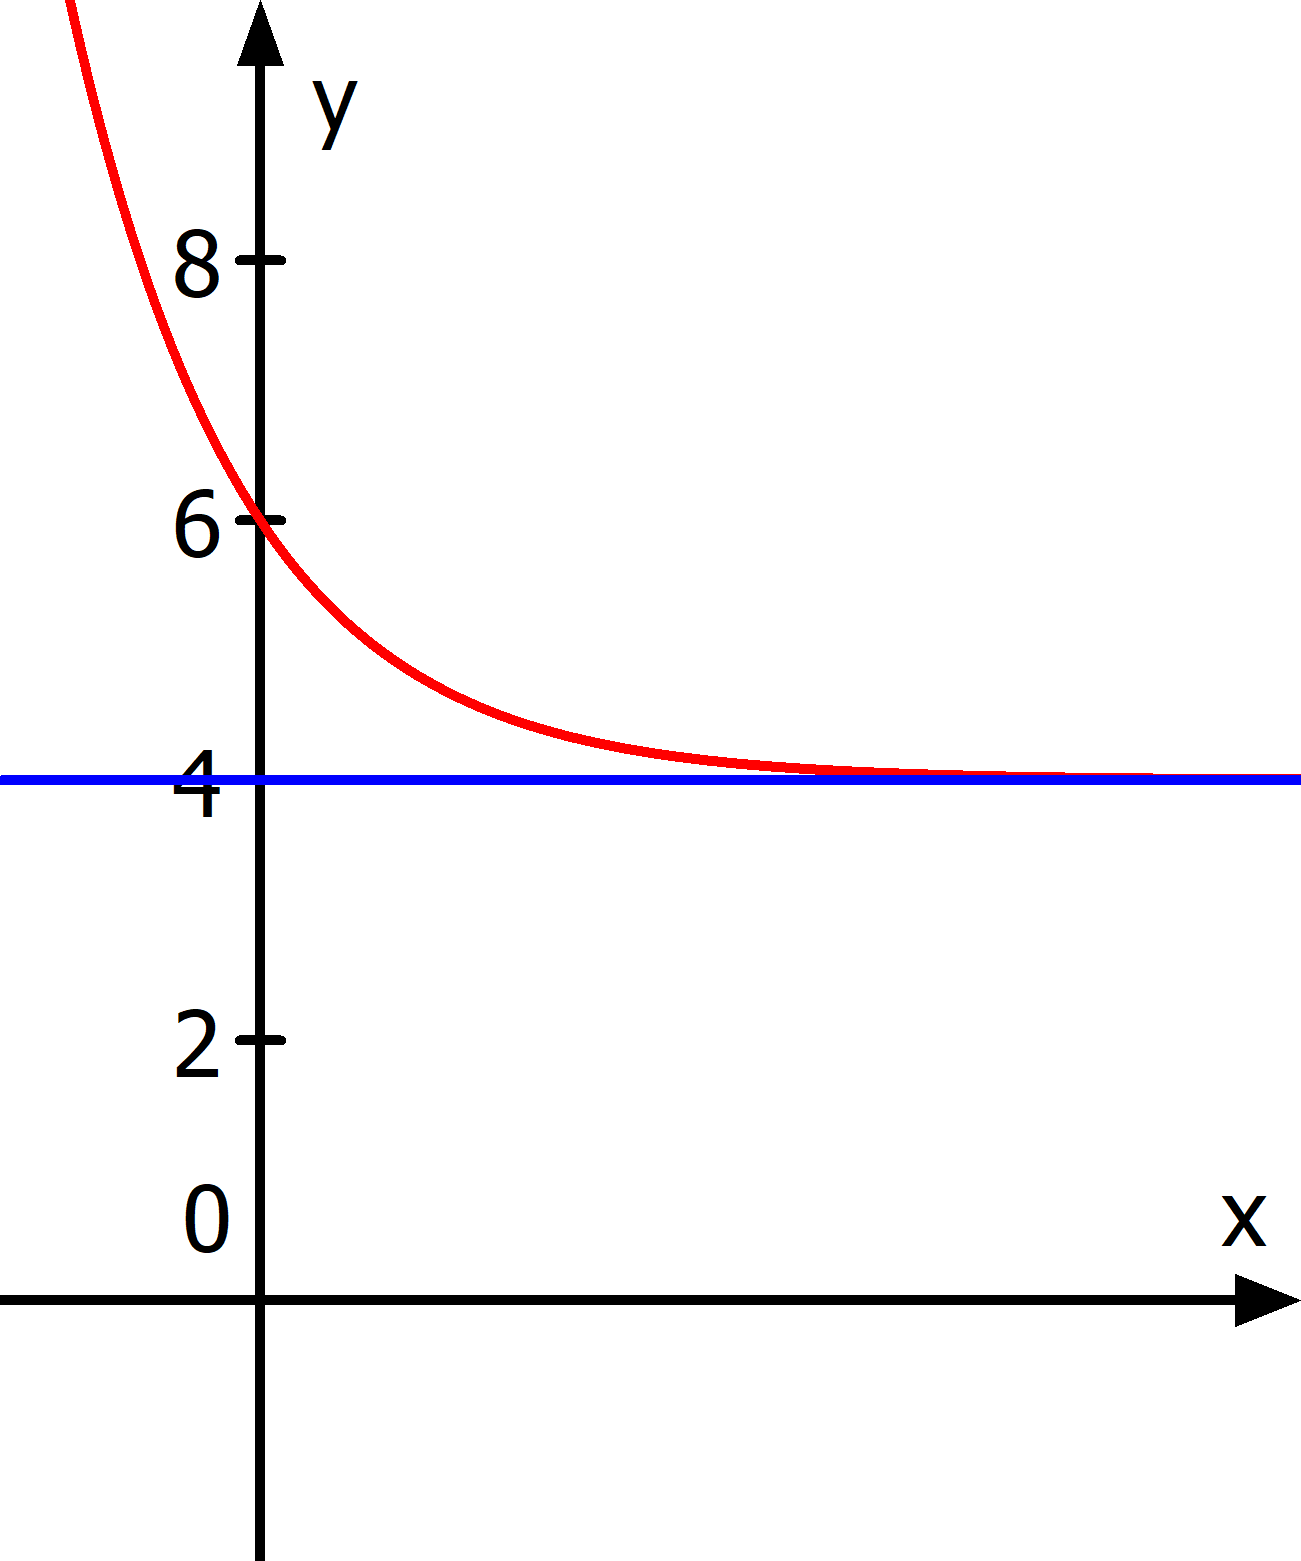
\includegraphics[width=.8\linewidth]{\eFkt/pics/A2o.png}
				\item \(f(x)=5e^{0,2x}-10\)

				Asymptote \(y=-10\)

				y-Achsenabschnitt: \(f(0)=-5\)

				Monoton wachsend

				\(f(x)\xrightarrow{\hphantom{\ }x\to-\infty\hphantom{\ }}-10\)

				\(f(x)\xrightarrow{\hphantom{\ }x\to\infty\hphantom{\ }}\infty\)

				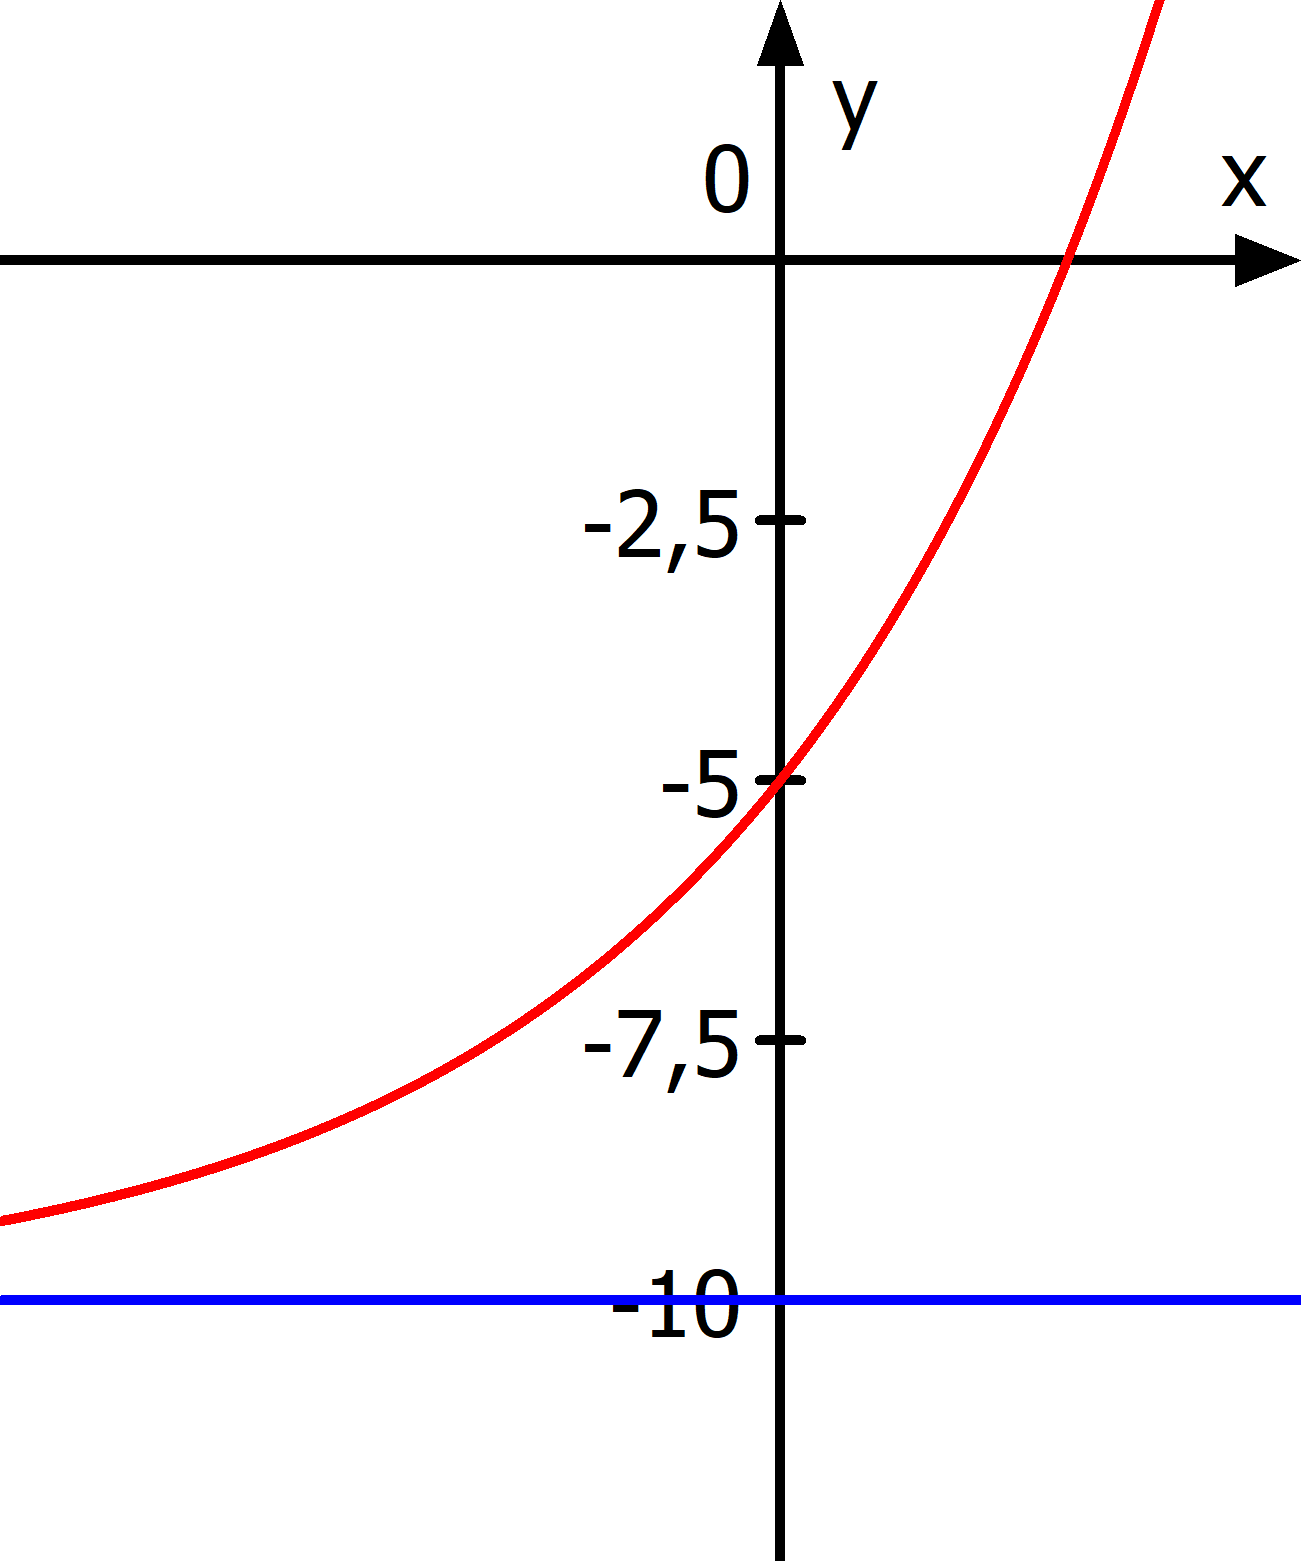
\includegraphics[width=.8\linewidth]{\eFkt/pics/A2p.png}
			\end{enumerate}
		\end{minipage}%
	\end{minipage}
	\newpage
	%%%%% q bis t
	\begin{minipage}{\textwidth}
		\begin{minipage}{0.5\textwidth}
			\begin{enumerate}[label=\alph*)]
				\setcounter{enumi}{16}
				\item \(f(x)=-\frac{1}{4}e^{-\frac{2}{3}x}+\frac{7}{4}\)

				Asymptote \(y=\frac{7}{4}\)

				y-Achsenabschnitt: \(f(0)=\frac{3}{2}\)

				Monoton wachsend

				\(f(x)\xrightarrow{\hphantom{\ }x\to-\infty\hphantom{\ }}-\infty\)

				\(f(x)\xrightarrow{\hphantom{\ }x\to\infty\hphantom{\ }}\frac{7}{4}\)

				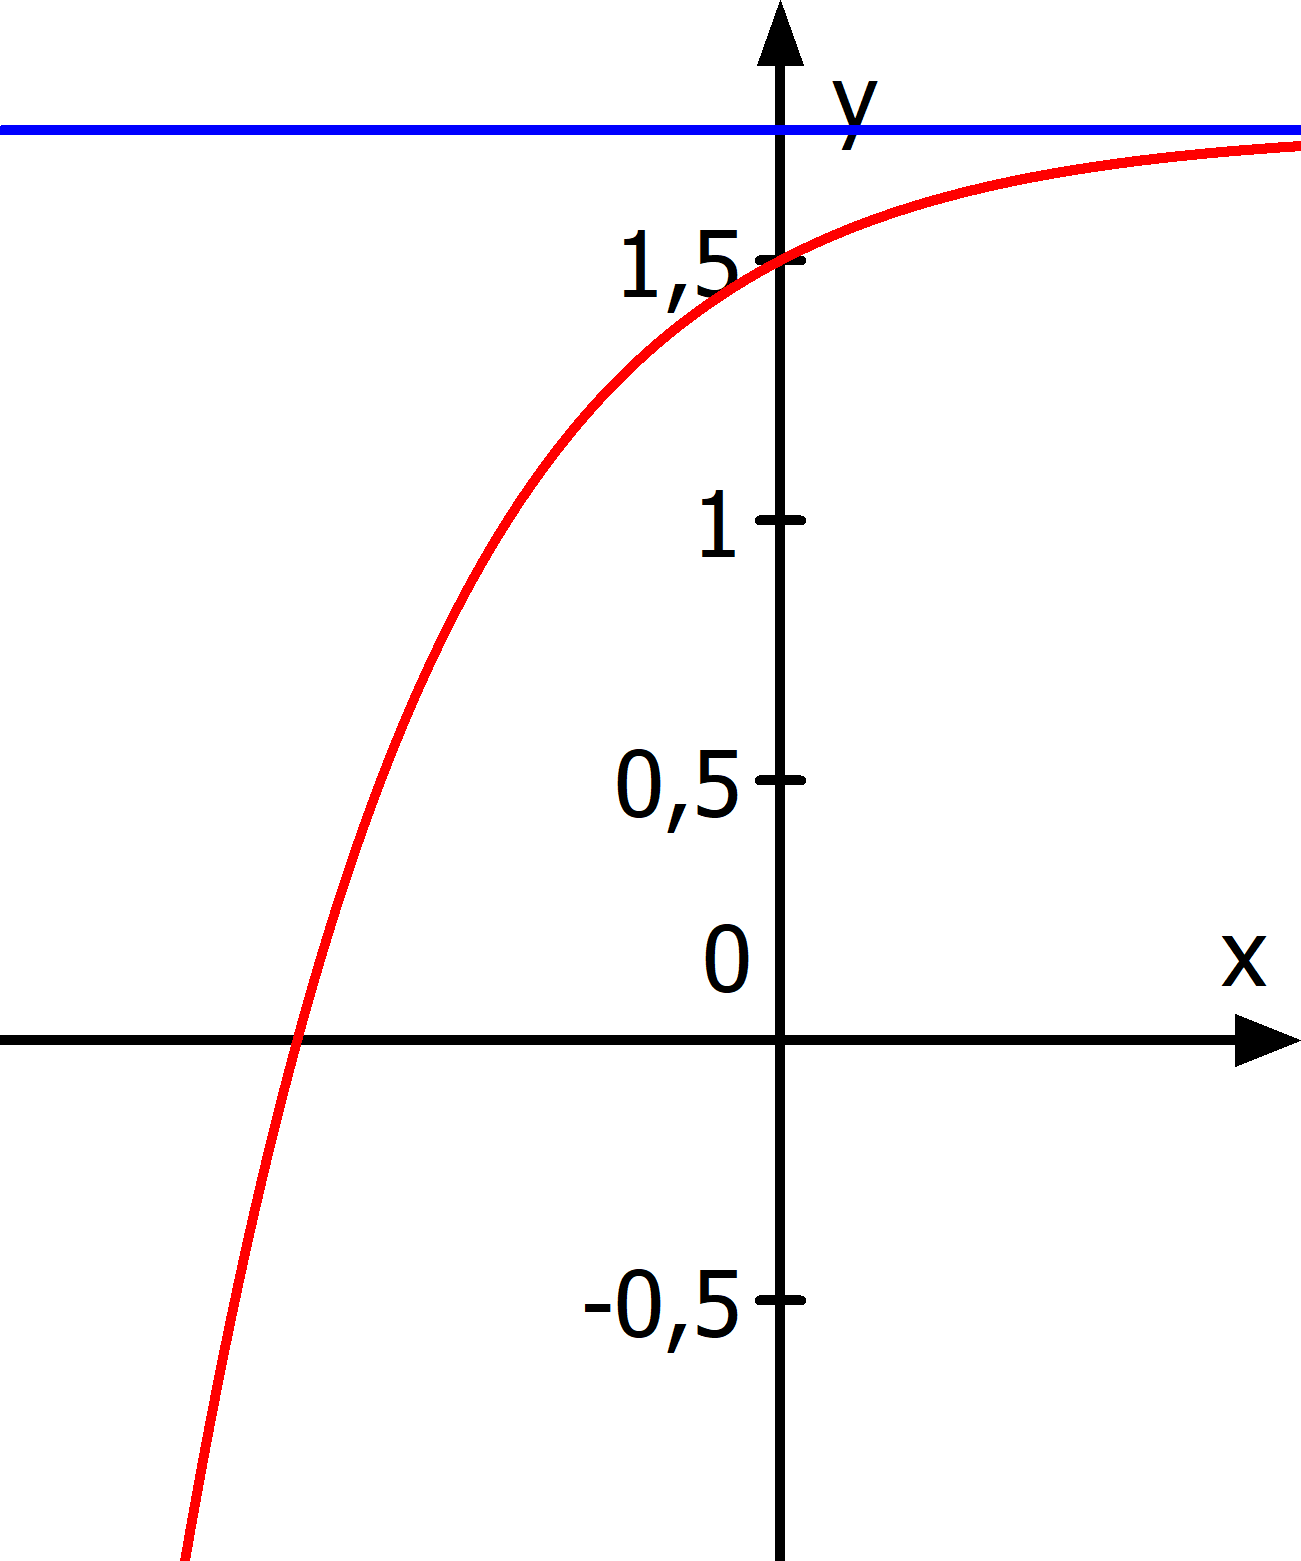
\includegraphics[width=.8\linewidth]{\eFkt/pics/A2q.png}
				\item \(f(x)=2e^{-0,2x}+3,5\)

				Asymptote \(y=3,5\)

				y-Achsenabschnitt: \(f(0)=5,5\)

				Monoton fallend

				\(f(x)\xrightarrow{\hphantom{\ }x\to-\infty\hphantom{\ }}\infty\)

				\(f(x)\xrightarrow{\hphantom{\ }x\to\infty\hphantom{\ }}3,5\)

				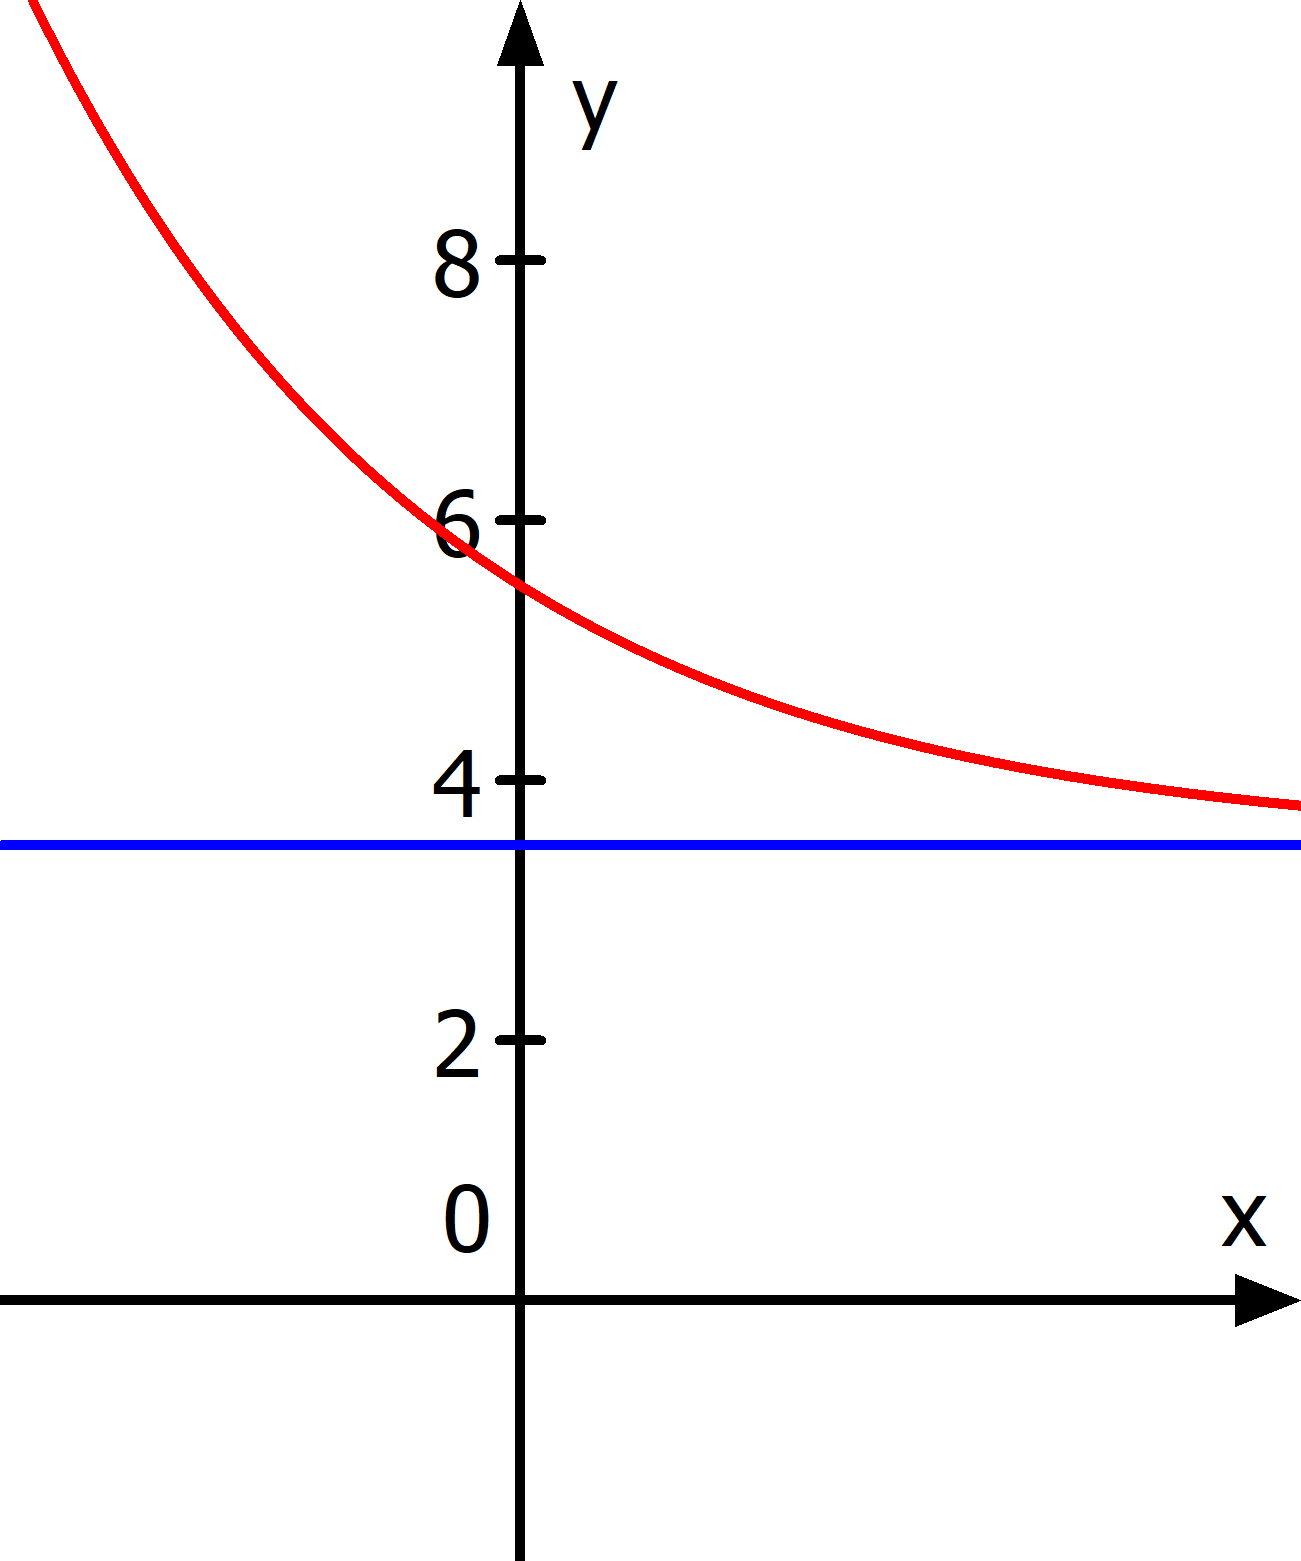
\includegraphics[width=.8\linewidth]{\eFkt/pics/A2r.png}
			\end{enumerate}
		\end{minipage}%
		\begin{minipage}{0.5\textwidth}
			\begin{enumerate}[label=\alph*)]
				\setcounter{enumi}{18}
				\item \(f(x)=e^{-4x}+3\)

				Asymptote \(y=3\)

				y-Achsenabschnitt: \(f(0)=4\)

				Monoton fallend

				\(f(x)\xrightarrow{\hphantom{\ }x\to-\infty\hphantom{\ }}\infty\)

				\(f(x)\xrightarrow{\hphantom{\ }x\to\infty\hphantom{\ }}3\)

				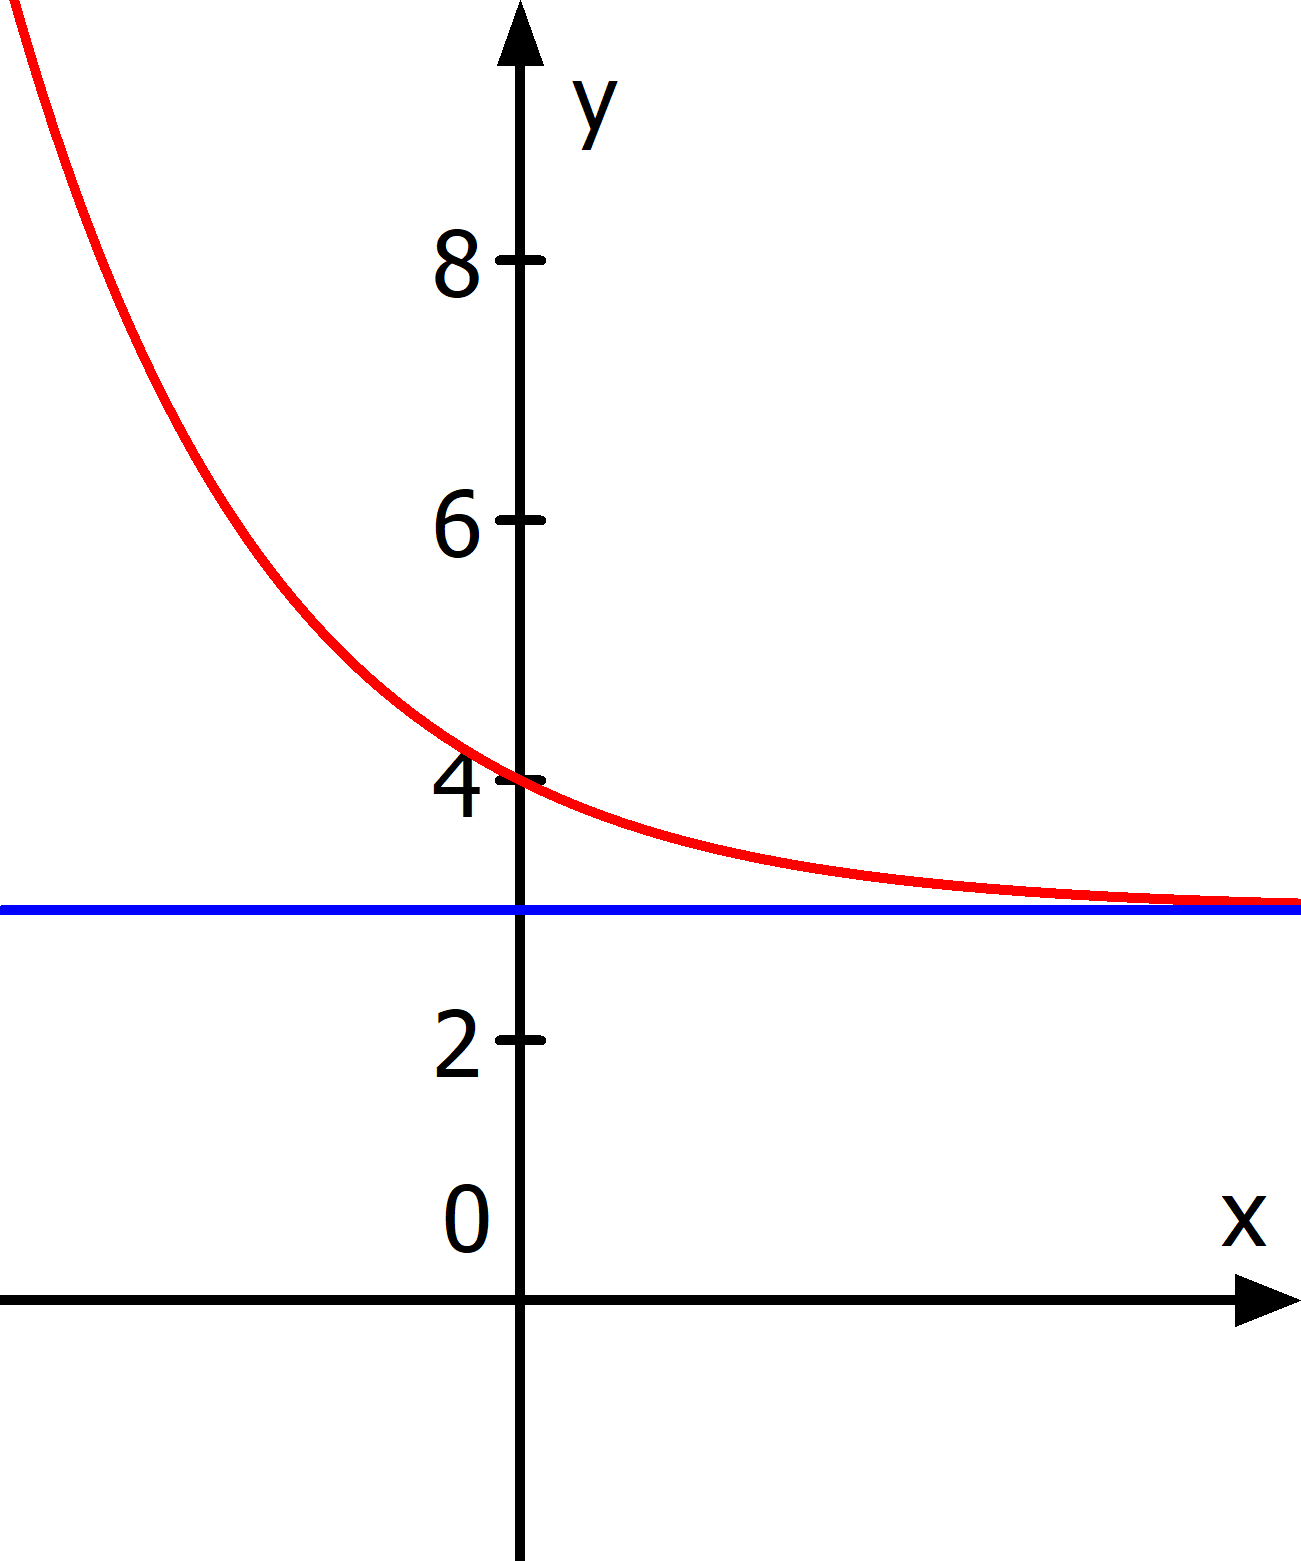
\includegraphics[width=.8\linewidth]{\eFkt/pics/A2s.png}
				\item \(f(x)=-4+5e^{7x}\)

				Asymptote \(y=-4\)

				y-Achsenabschnitt: \(f(0)=1\)

				Monoton wachsend

				\(f(x)\xrightarrow{\hphantom{\ }x\to-\infty\hphantom{\ }}-4\)

				\(f(x)\xrightarrow{\hphantom{\ }x\to\infty\hphantom{\ }}\infty\)

				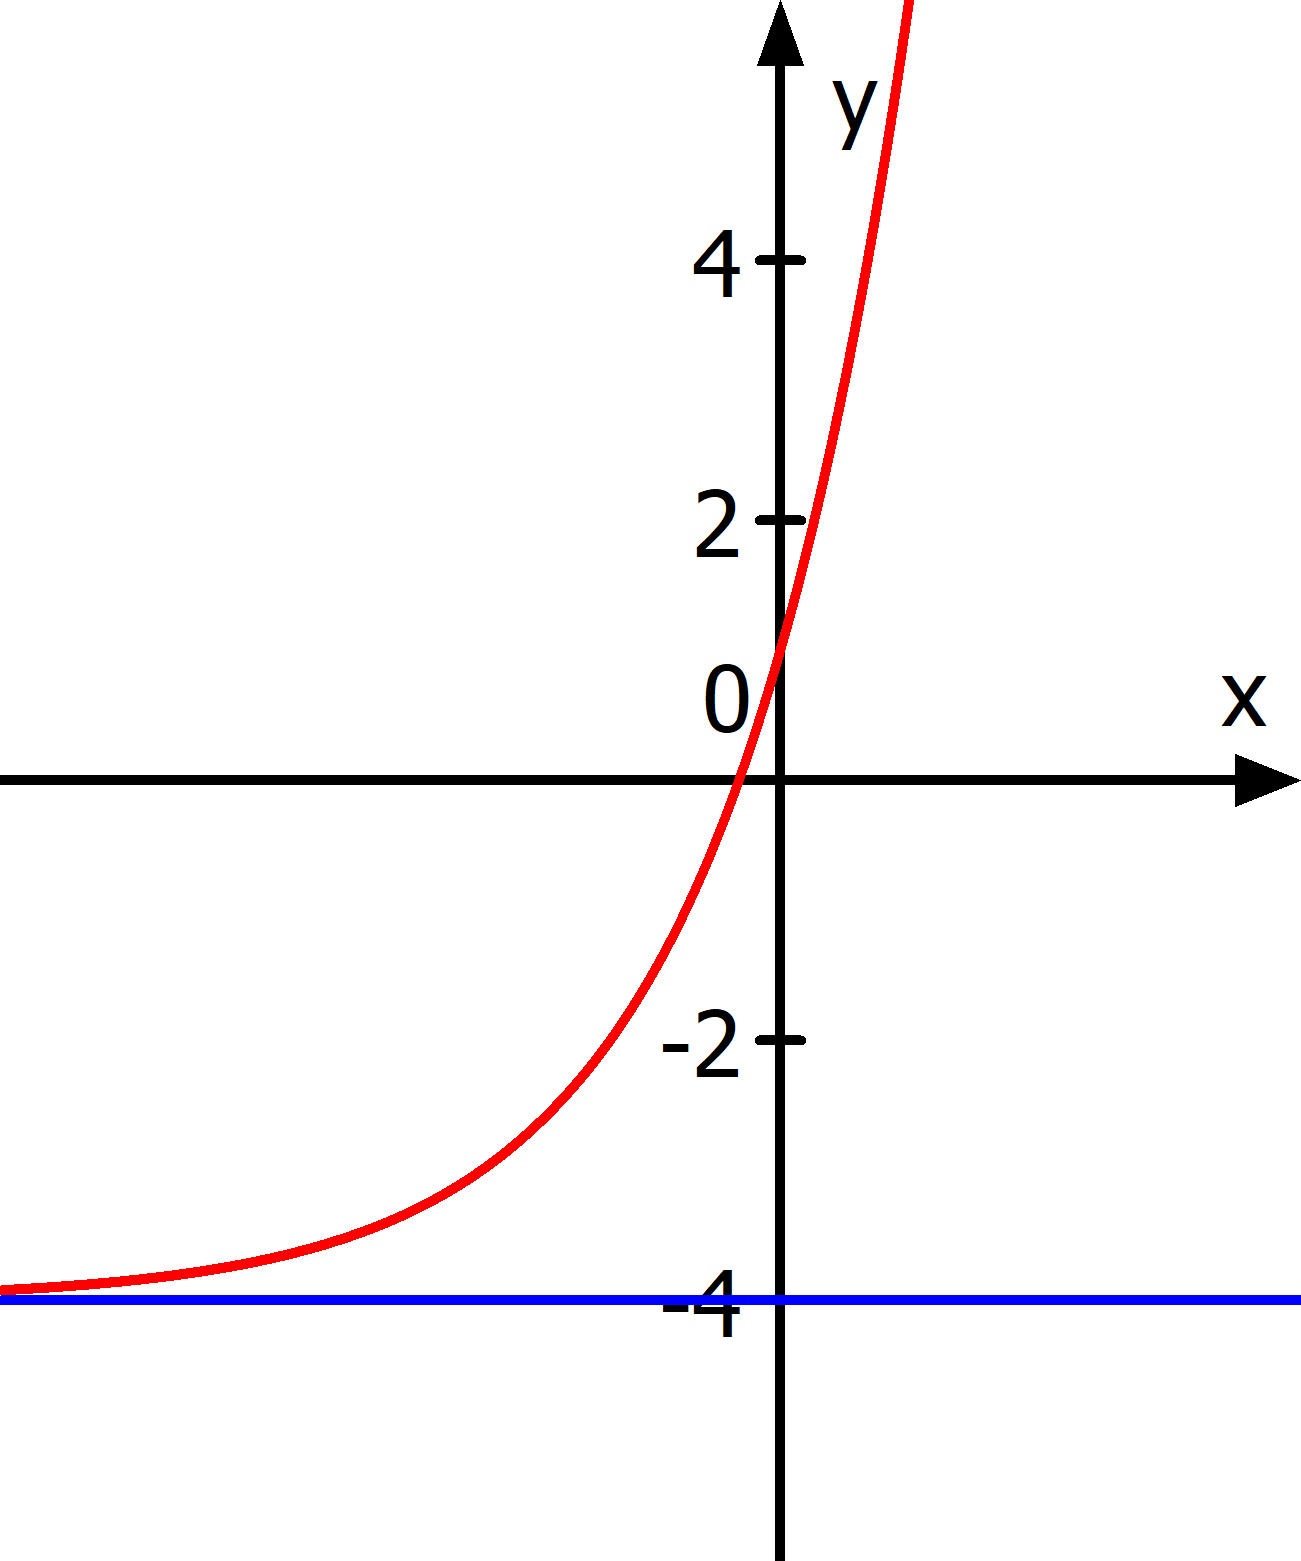
\includegraphics[width=.8\linewidth]{\eFkt/pics/A2t.png}
			\end{enumerate}
		\end{minipage}%
	\end{minipage}
	\newpage
	%%%%% u bis t
	\begin{minipage}{\textwidth}
		\begin{minipage}{0.5\textwidth}
			\begin{enumerate}[label=\alph*)]
				\setcounter{enumi}{20}
				\item \(f(x)=\frac{3}{2}-\frac{9}{4}e^{\frac{3}{8}x}\)

				Asymptote \(y=\frac{3}{2}\)

				y-Achsenabschnitt: \(f(0)=-\frac{3}{4}\)

				Monoton fallend

				\(f(x)\xrightarrow{\hphantom{\ }x\to-\infty\hphantom{\ }}\frac{3}{2}\)

				\(f(x)\xrightarrow{\hphantom{\ }x\to\infty\hphantom{\ }}-\infty\)

				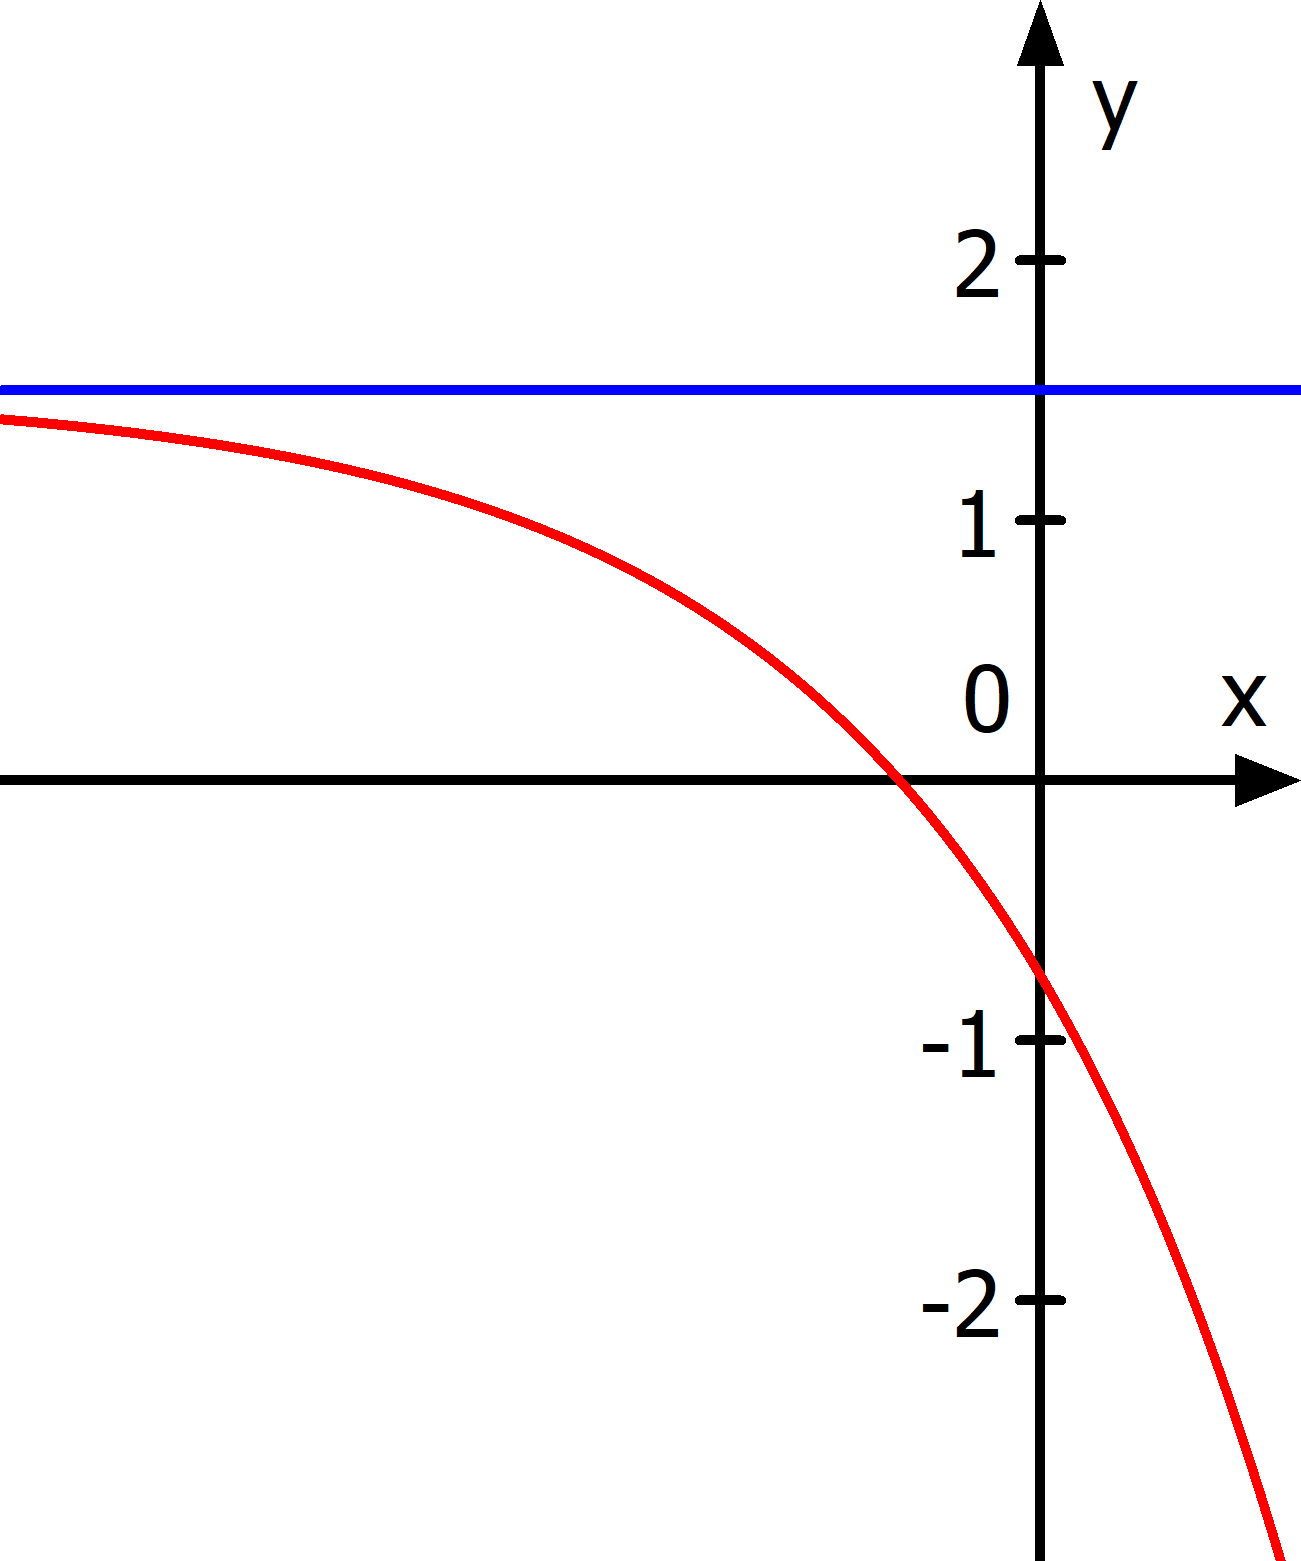
\includegraphics[width=.8\linewidth]{\eFkt/pics/A2u.png}
				\item \(f(x)=-2\left(1+e^{-0,3x}\right) \)

				Asymptote \(y=-2\)

				y-Achsenabschnitt: \(f(0)=-4\)

				Monoton wachsend

				\(f(x)\xrightarrow{\hphantom{\ }x\to-\infty\hphantom{\ }}-\infty\)

				\(f(x)\xrightarrow{\hphantom{\ }x\to\infty\hphantom{\ }}-2\)

				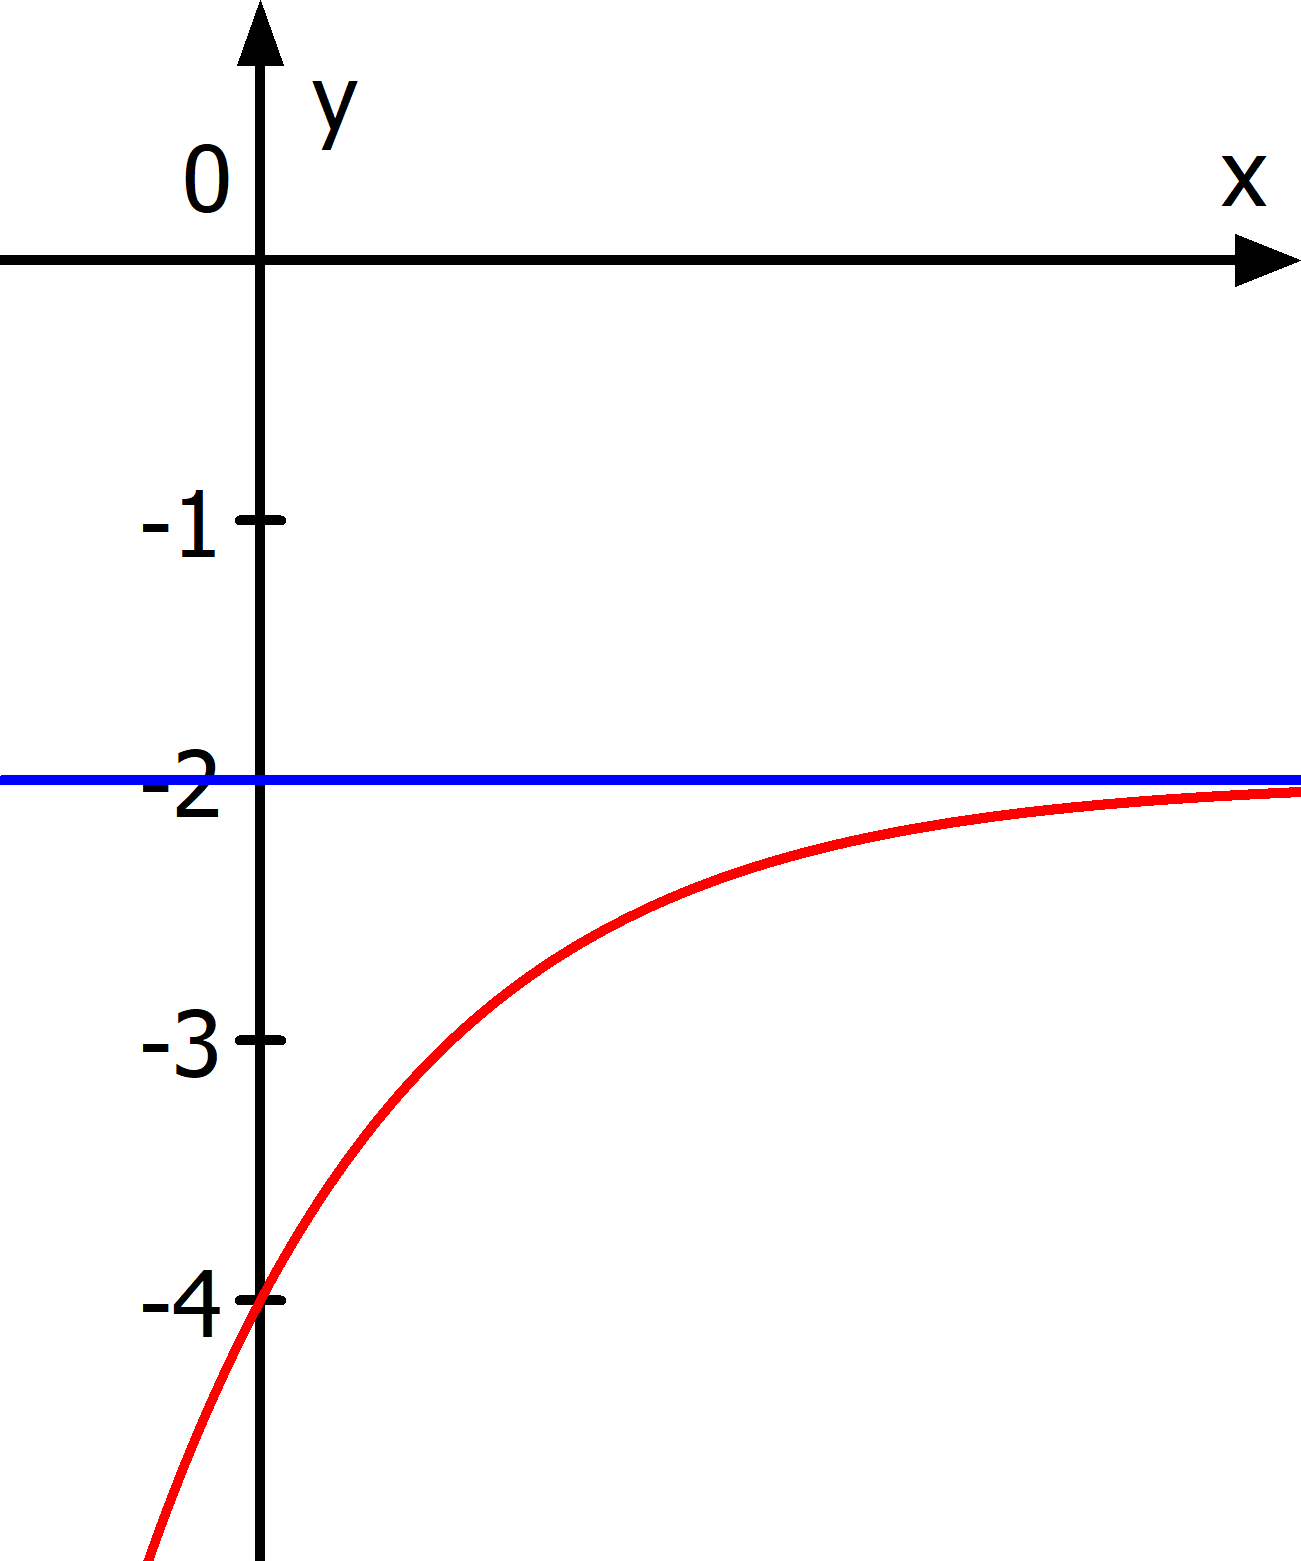
\includegraphics[width=.8\linewidth]{\eFkt/pics/A2v.png}
			\end{enumerate}
		\end{minipage}%
		\begin{minipage}{0.5\textwidth}
			\begin{enumerate}[label=\alph*)]
				\setcounter{enumi}{22}
				\item \(f(x)=5\left(e^{-4x}+\frac{1}{2}\right) \)

				Asymptote \(y=\frac{5}{2}\)

				y-Achsenabschnitt: \(f(0)=\frac{15}{2}=7,5\)

				Monoton fallend

				\(f(x)\xrightarrow{\hphantom{\ }x\to-\infty\hphantom{\ }}\infty\)

				\(f(x)\xrightarrow{\hphantom{\ }x\to\infty\hphantom{\ }}\frac{5}{2}\)

				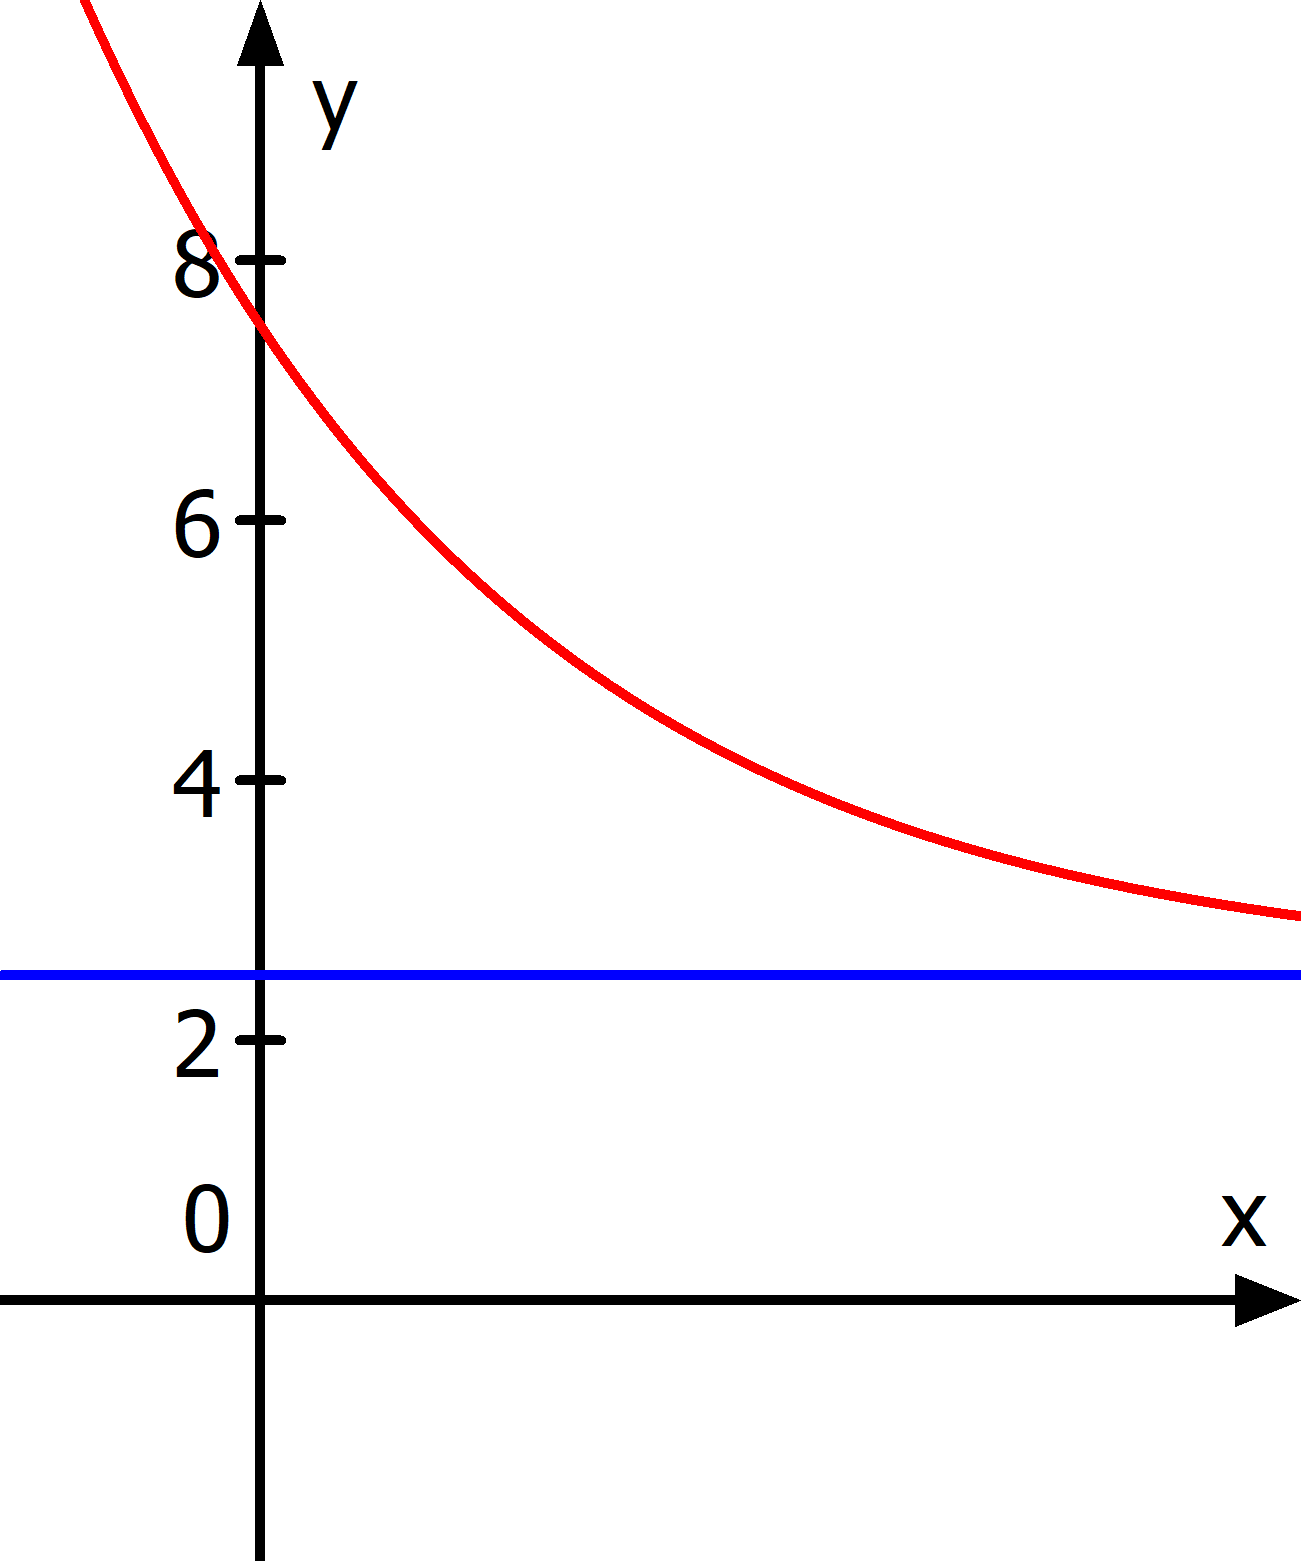
\includegraphics[width=.8\linewidth]{\eFkt/pics/A2w.png}
				\item \(f(x)=-2\left( 2e^{6x}-2\right) \)

				Asymptote \(y=4\)

				y-Achsenabschnitt: \(f(0)=0\)

				Monoton fallend

				\(f(x)\xrightarrow{\hphantom{\ }x\to-\infty\hphantom{\ }}4\)

				\(f(x)\xrightarrow{\hphantom{\ }x\to\infty\hphantom{\ }}-\infty\)

				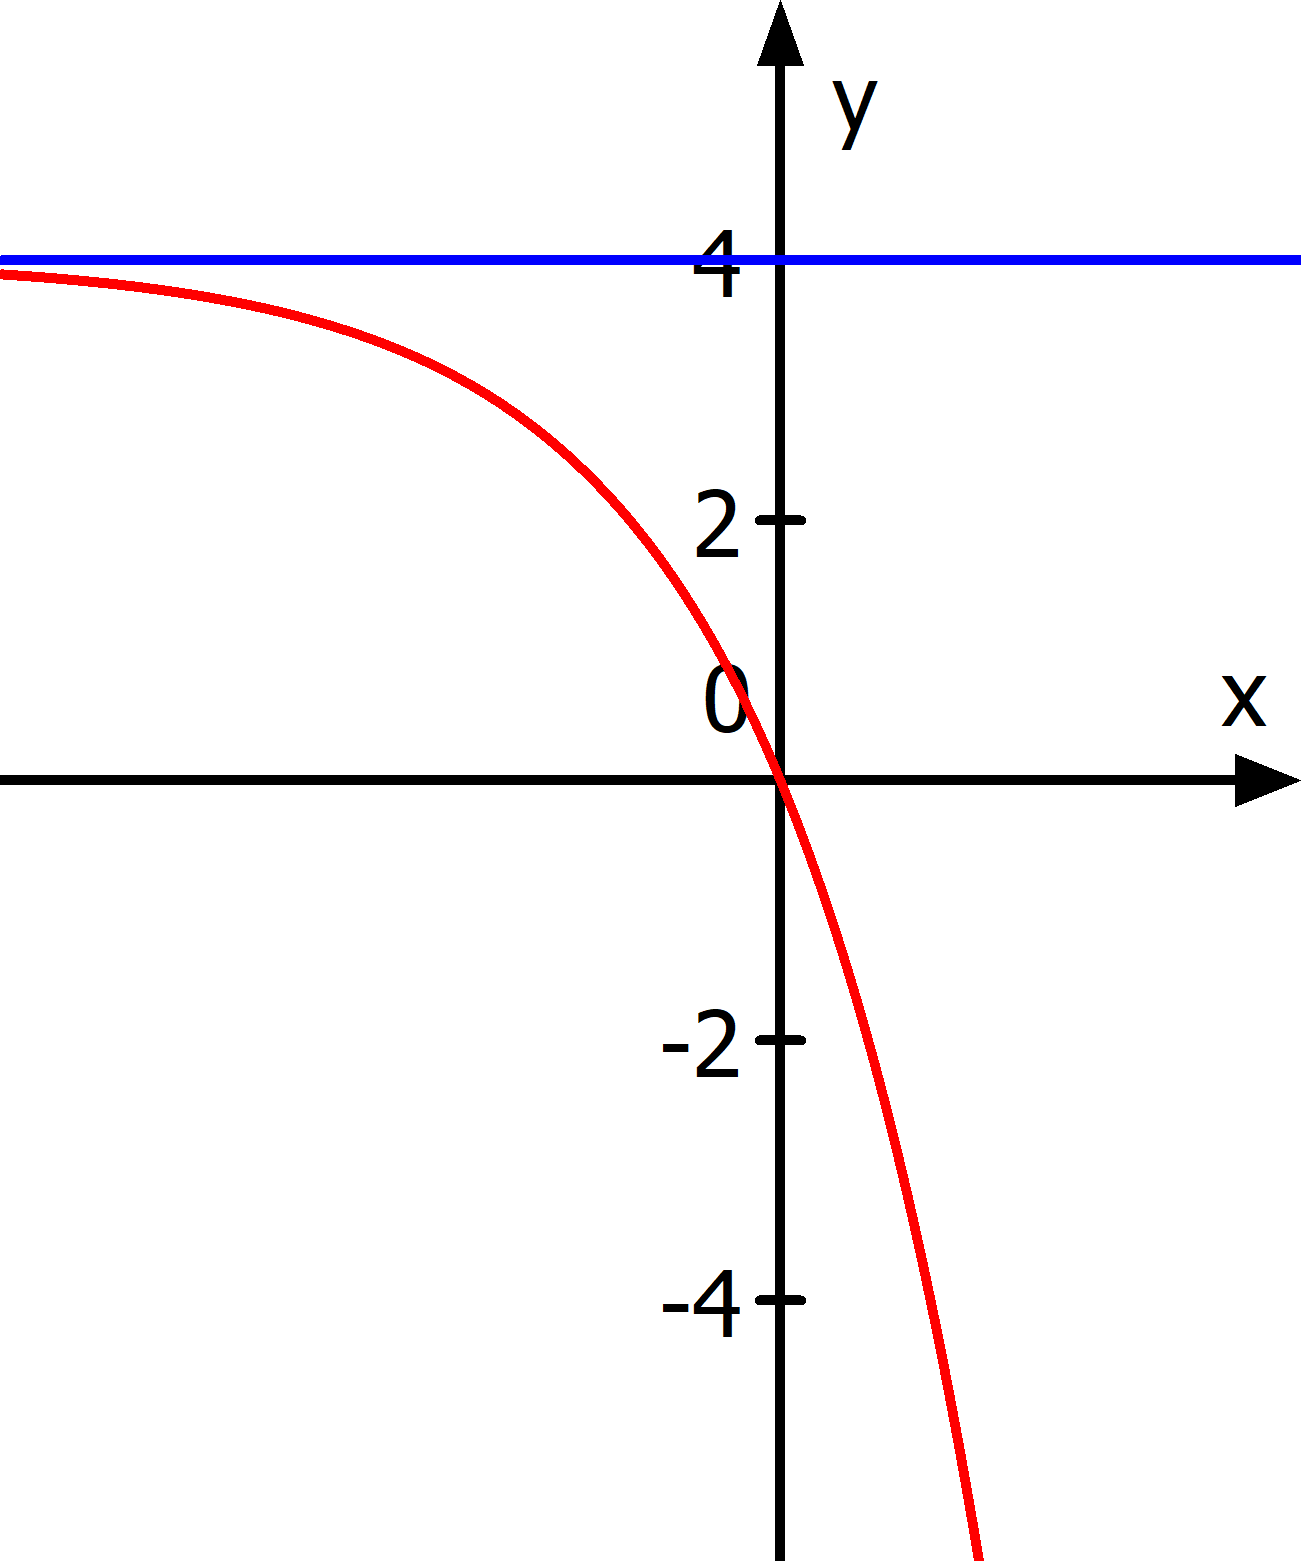
\includegraphics[width=.8\linewidth]{\eFkt/pics/A2x.png}
			\end{enumerate}
		\end{minipage}%
	\end{minipage}
	\newpage
	%%%%% y und z
	\begin{minipage}{\textwidth}
		\begin{minipage}{0.5\textwidth}
			\begin{enumerate}[label=\alph*)]
				\setcounter{enumi}{24}
				\item \(f(x)=-e^{-1,1x}+3\left(e^{-1,1x}-2\right)\)

				Asymptote \(y=-6\)

				y-Achsenabschnitt: \(f(0)=-4\)

				Monoton fallend

				\(f(x)\xrightarrow{\hphantom{\ }x\to-\infty\hphantom{\ }}\infty\)

				\(f(x)\xrightarrow{\hphantom{\ }x\to\infty\hphantom{\ }}-6\)

				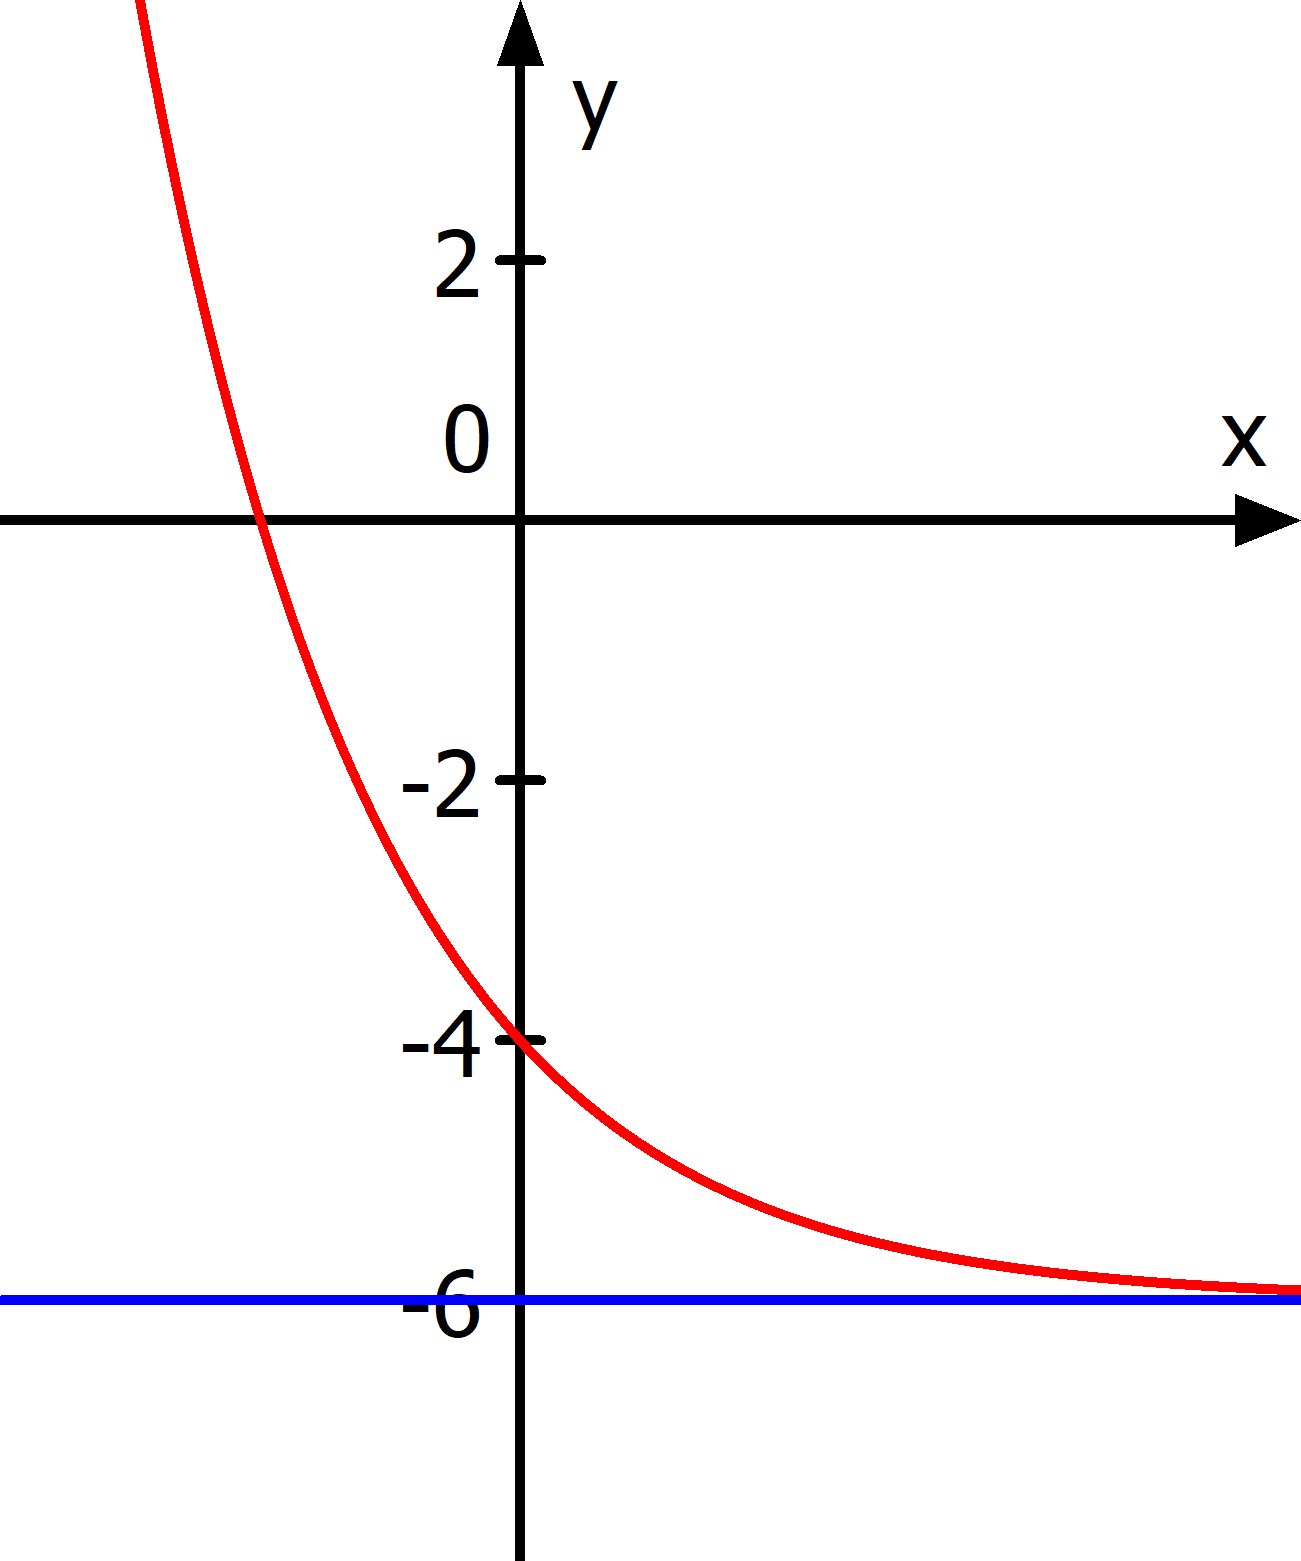
\includegraphics[width=.8\linewidth]{\eFkt/pics/A2y.png}
			\end{enumerate}
		\end{minipage}%
		\begin{minipage}{0.5\textwidth}
			\begin{enumerate}[label=\alph*)]
				\setcounter{enumi}{25}
				\item \(f(x)=4\left( 0,25e^{1,25x}+2\right) -8\)

				Asymptote \(y=0\)

				y-Achsenabschnitt: \(f(0)=1\)

				Monoton wachsend

				\(f(x)\xrightarrow{\hphantom{\ }x\to-\infty\hphantom{\ }}0\)

				\(f(x)\xrightarrow{\hphantom{\ }x\to\infty\hphantom{\ }}\infty\)

				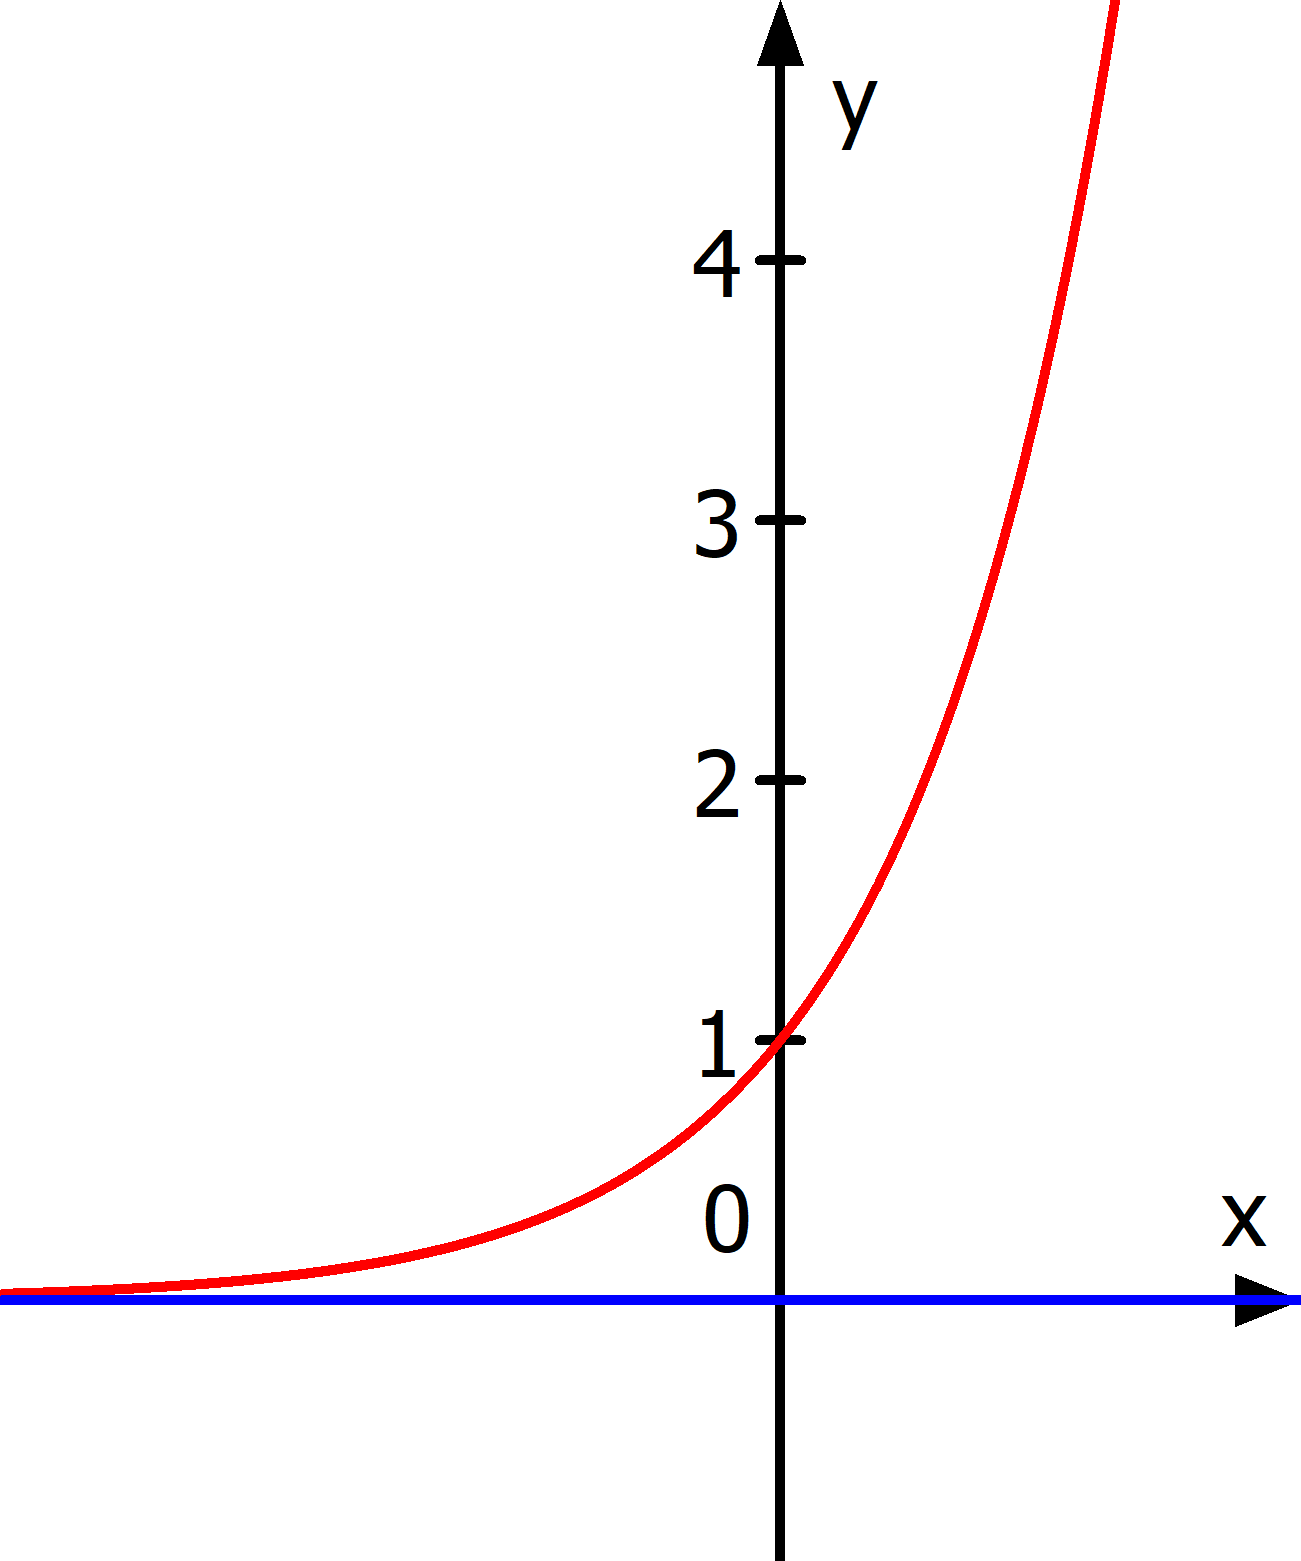
\includegraphics[width=.8\linewidth]{\eFkt/pics/A2z.png}
			\end{enumerate}
		\end{minipage}%
	\end{minipage}
\end{Answer}